% Shared preamble for the CIG-AMF formal-research papers.
% IEEEtran conference class; compiles on Overleaf without modification.
\documentclass[conference]{IEEEtran}
\IEEEoverridecommandlockouts

\usepackage{cite}
\usepackage{amsmath,amssymb,amsfonts}
\usepackage{amsthm}
\usepackage{algorithm}
\usepackage{algorithmic}
\usepackage{graphicx}
\usepackage{textcomp}
\usepackage{xcolor}
\usepackage{booktabs}
\usepackage{url}
\usepackage[hidelinks]{hyperref}

\def\BibTeX{{\rm B\kern-.05em{\sc i\kern-.025em b}\kern-.08em T\kern-.1667em\lower.7ex\hbox{E}\kern-.125emX}}

\newtheorem{theorem}{Theorem}
\newtheorem{lemma}[theorem]{Lemma}
\newtheorem{proposition}[theorem]{Proposition}
\newtheorem{corollary}[theorem]{Corollary}
\theoremstyle{definition}
\newtheorem{definition}[theorem]{Definition}
\newtheorem{remark}[theorem]{Remark}
\newtheorem{example}[theorem]{Example}

% A machine-checked statement carries its Lean declaration name.
\newcommand{\lean}[1]{\textsf{\footnotesize #1}}
\newcommand{\leanbox}[1]{%
  \par\vspace{2pt}\noindent
  {\footnotesize\textsf{Lean: #1}}\par\vspace{2pt}}

% Evidence classes, used consistently and never interchangeably.
\newcommand{\PROVED}{\textsc{proved}}
\newcommand{\CERT}{\textsc{certificate}}
\newcommand{\NUM}{\textsc{numerical}}
% figures resolve both in the repository layout and in a flat Overleaf bundle
\graphicspath{{../_figures/}{figures/}{./}}

% ---------------------------------------------------------------------------
% Draft notes.  Blue is information carried forward for the final write-up;
% red is a decision or a gap that still needs an author.  Both disappear from
% the whole document with one line -- put \shownotesfalse here when the draft
% becomes the submission, and nothing else has to be edited.
% ---------------------------------------------------------------------------
\newif\ifshownotes\shownotestrue
\definecolor{notecol}{RGB}{0,70,190}
\definecolor{todocol}{RGB}{190,20,20}
\newcommand{\NOTE}[1]{\ifshownotes{\color{notecol}\,\textsf{\footnotesize[N: #1]}}\fi}
\newcommand{\TODO}[1]{\ifshownotes{\color{todocol}\,\textsf{\footnotesize[TODO: #1]}}\fi}
% a standalone paragraph-level note, for longer remarks between paragraphs
\newcommand{\NOTEPAR}[1]{\ifshownotes\par\vspace{2pt}\noindent%
  {\color{notecol}\textsf{\footnotesize\textbf{Note.}\;#1}}\par\vspace{2pt}\fi}
\newcommand{\TODOPAR}[1]{\ifshownotes\par\vspace{2pt}\noindent%
  {\color{todocol}\textsf{\footnotesize\textbf{To decide.}\;#1}}\par\vspace{2pt}\fi}


\begin{document}

\title{The Slice Is Not a Restriction, the Design Is Not Fitted,\\
and the Margin Threshold Is Sharp}

\author{\IEEEauthorblockN{Vu Phan An Nguyen}
\IEEEauthorblockA{\textit{Rider University} \\
Lawrenceville, NJ, USA}}

\maketitle

\begin{abstract}
A scalar query measures $q$ coordinates and must distinguish the truth from an alternative.
Its per-sample information is customarily stated against an alternative parameterised by
$(d,x)$: $d$ coordinates displaced by $\mu$, the remaining $q-d$ displaced by $x$. Two
objections stand against using that statement, and neither is answered by more cells or more
search. A bound proved only over a two-parameter \emph{slice} says nothing about alternatives
outside it, so a lower bound quantified over $(d,x)$ is not a lower bound over the class; and
the design weights reproducing the corpus's coefficients were \emph{fitted}, so a consistent
non-negative solution in $24$ of $24$ cells is evidence rather than a derivation. This paper
supplies an argument for each. We define the general alternative as an arbitrary shift
vector, show the $(d,x)$ formula is exactly the general information evaluated on the slice,
and prove that every alternative in the class costs at least the slice value, with equality
attained on the slice---so the reduction loses nothing and gains nothing. The same
computation shows the general information vanishes only at the zero shift, so the scalar
query is blind in no direction. We then prove that the budget constraint together with the
split \emph{forces} the two weights, which depend on the split and the price alone and not on
the model parameters; the delivered information is consequently affine in the split, so the
optimum sits at an endpoint unless the two queries buy information at exactly the same rate
per unit price. Finally we prove a margin-sensitive exchange bound
$2(L_{F}(T)-L_{F}(S))\le|T\setminus S|(2\delta-\mu)$ with no symmetry or fixed-cell
assumption, and from it a \emph{sharp threshold}: a margin of $2\delta$ is sufficient for
Top-$C$ optimality under every product reference, and for every margin below it an explicit
construction makes Top-$C$ strictly suboptimal. Each displayed theorem is machine-checked in
Lean~4 with no \texttt{sorry}. Sufficiency is proved for every product reference and
necessity only at the corner; an exact rational sweep between them, validated against the
proved identity before being reported, finds the construction degrading continuously rather
than collapsing, and failing only past a breakdown point that grows with the margin and is
never reached at the threshold.
\end{abstract}

\begin{IEEEkeywords}
experimental design, information bounds, alternative families, budget allocation,
approximate modularity, formal verification
\end{IEEEkeywords}

\section{Introduction}

A scalar query measures $q$ coordinates at once and returns a noisy scalar summary. To
certify an answer it must distinguish the truth from an alternative, and the standard way to
state what it can do is to fix a two-parameter family of alternatives---$d$ coordinates
displaced by $\mu$, the remaining $q-d$ by $x$---and compute the per-sample information
$I_{B}(d,x)$ against that family.

This is convenient, and it is what a corpus of results is stated against. It is also open to
two objections that no amount of further computation answers.

The first is about quantifiers. A lower bound proved by quantifying over $(d,x)$ is a lower
bound over a two-dimensional slice of a $q$-dimensional class. An alternative outside the
slice is not covered, and for all the bound says it could be cheaper. Using such a bound as
though it were class-quantified is a quantifier error, and it is repaired by an argument or
not at all: no finite collection of alternatives sampled from outside the slice establishes a
universal claim.

The second is about provenance. The design weights reproducing the corpus's coefficients were
obtained by fitting. A consistent non-negative solution in $24$ of $24$ parameter cells is
good evidence that the coefficients come from the model rather than from the fit; it is not a
derivation, and the difference matters if the weights are to be used outside the cells
tested. This objection too is not closed by more cells, since the existing cells were already
consistent.

The paper makes five contributions. First, it shows the slice is not a restriction: every
alternative in the class costs at least the slice value. Second, it shows the slice is exactly
tight, so the reduction is lossless. Third, it shows the general information vanishes only at
the zero shift, so the scalar query has no blind direction---which is what makes a mixed
design with the pair query an interesting question at all. Fourth, it derives the design from
the budget and the split rather than fitting it, and draws the consequence that the delivered
information is affine, so the optimum is pure except on an explicitly computable threshold.
Fifth, it proves a margin-sensitive exchange bound and the sharp threshold that follows from
it.

The scope is bounded. The reduction is for the scalar query, whose information is separable
across coordinates; the pair query has a blind direction and is not covered. The reduction
converts a \emph{lower} bound only. And the necessity half of the sharp threshold uses the
corner reference, for a reason Section~\ref{sec:threshold} states and quantifies rather than
leaves implicit.

\section{Background}

\subsection{Alternative Families in Design and Testing}

Reducing a high-dimensional alternative class to a low-dimensional family is an old device.
In optimal design it appears as the restriction of the criterion to a parametric direction
\cite{pukelsheim2006,fedorov1972}; in testing it appears as the choice of a least-favourable
alternative. The device is sound when the restriction is shown to be extremal, and unsound
when it is merely convenient.

However, that distinction is not always drawn, and it is exactly what the slice objection
raises. A family chosen for computability may or may not contain the minimiser, and the
descriptions in the literature are typically constructive---``$d$ coordinates at $\mu$ and
the rest at $x$''---which gives no indication whether the family is a restriction or an
extreme point of something larger. This paper settles the status for one case:
Theorem~\ref{thm:reduction} shows the family is extremal within the magnitude-constrained
class, and Corollary~\ref{cor:tight} that it is exactly so.

\subsection{Budget-Constrained Allocation}

Allocating a budget between measurement types under a linear price is a standard convex
programme \cite{boyd2004}, and the affine structure of Theorem~\ref{thm:affine} is a special
case of the observation that a linear objective over a simplex attains its optimum at a
vertex.

What is specific here is that the reduction to an affine objective is not assumed but
derived. It follows from Theorem~\ref{thm:unique}, which removes the apparent freedom in the
weights and leaves the split as the only variable. Without that step one optimises over a
two-dimensional weight space subject to one budget constraint, and the objective on that
space is linear but the feasible set is a segment whose parameterisation is not obviously the
split. Fixing the parameterisation is what makes the transition condition readable as ``equal
information per unit price'' rather than as an arbitrary algebraic condition.

\subsection{Approximate Modularity and Exchange Bounds}

The exchange bound of Section~\ref{sec:margin} sits near the literature on approximately
modular set functions, which studies how far a function can be from additive and what that
costs for optimisation; Feige, Feldman and Talgam-Cohen give stability and approximation
results for that class \cite{feige2020}, and the general theory of decompositions for
categorical inputs is well developed.

However, ``nearly additive'' is not by itself a source of novelty here, and the distinction
must be drawn on three axes rather than claimed. The modulus is different: $\delta$ bounds
mixed differences of $F$ under a product reference, not a global additivity defect. The
reference is different and, as Section~\ref{sec:threshold} shows, decisive---the necessity
construction is stated at the corner, and the sweep of Section~\ref{sec:results} measures how
far from the corner it survives. And the loss is a decision loss over
Top-$C$ selection rather than an approximation error. What this paper contributes is the
margin term: the bound $2|T\setminus S|\delta$ that an endpoint-patch argument gives is
improved to $|T\setminus S|(2\delta-\mu)$ by retaining a score surplus that the earlier
argument discarded.

\subsection{Interval and Rational Certificates}

The enclosure discipline of Section~\ref{sec:certificate} is standard interval arithmetic
\cite{moore2009} carried out over the rationals so that the enclosures are exact rather than
outward-rounded floats. Nothing about the technique is new; it is used because the
conclusions are strict inequalities, and a strict inequality established in floating point is
not established.

\subsection{The Gap}

The literature therefore leaves a specific opening. Design theory uses restricted alternative
families without always settling whether they are extremal; budget allocation gives vertex
optima but not a derivation of the weights that makes the objective affine; approximate
modularity gives exchange bounds but under a different modulus, reference and loss. No
existing treatment simultaneously: (i) proves a constructive alternative family extremal and
exactly tight; (ii) derives the design weights from the budget rather than fitting them;
(iii) retains the score surplus in the exchange bound so that a margin appears explicitly;
and (iv) exhibits a sharp threshold at which Top-$C$ selection stops being optimal.

\section{Research Aims, Questions, and Hypotheses}

\subsection{Research Aim}

The aim of this work is to settle the status of two ingredients that a corpus of information
bounds currently carries without argument---the restricted alternative family and the fitted
design---and to determine the exact margin at which Top-$C$ selection ceases to be optimal.

\subsection{Research Questions}

\begin{itemize}
\item \textbf{RQ1.} Is the two-parameter alternative family extremal within the
magnitude-constrained class, so that a slice-quantified lower bound is class-quantified?
\item \textbf{RQ2.} Are the design weights forced by the budget and the split, or is there
residual freedom that a fit is choosing?
\item \textbf{RQ3.} Where can the optimal design change character as the split varies?
\item \textbf{RQ4.} At what margin does Top-$C$ selection stop being optimal, and is that
threshold sharp?
\end{itemize}

\subsection{Hypotheses}

\begin{itemize}
\item \textbf{H1.} Because the class is cut out by \emph{lower} bounds on coordinate
magnitudes and the objective increases in each, the minimiser is where every constraint is
active, which is the slice.
\item \textbf{H2.} The budget is one linear equation and the split supplies a second, so the
weight pair is determined and depends on $(\eta,c)$ alone.
\item \textbf{H3.} With the weights determined, the delivered information is affine in the
split, so the optimum is at an endpoint unless the slope vanishes.
\item \textbf{H4.} A margin of $2\delta$ is sufficient for Top-$C$ optimality, and below it
an explicit construction attains the exchange bound with equality, making the threshold
sharp.
\end{itemize}

\section{Methodology}
\label{sec:setting}

\subsection{Framework Overview}

The \emph{class} of alternatives is cut out by per-coordinate magnitude constraints: a shift
$v\in\mathbb{R}^{q}$ belongs to the class determined by $(S,\mu,x)$ when $|v_{i}|\ge\mu$ for
$i\in S$ and $|v_{i}|\ge x$ for $i\notin S$, with $|S|=d$. The slice is the sub-family in
which every inequality holds with equality and every sign agrees.

For the margin results we additionally write $\mathrm{osc}(f)=\max f-\min f$, $Q_{j}$ for the
product response of coordinate $j$ under a product reference, and $L_{F}(S)$ for the
compression loss of retaining the coordinate set $S$.

A distinction is maintained throughout. The information formulas $I_{B}$ and
$I_{\mathrm{pair}}$ are taken as given from the corpus and are not re-derived from the
sampling model. The paper's subject is what can be concluded \emph{from} them, and a reader
who disputes them disputes the premises rather than the argument.

\subsection{Simplifying Assumptions}
\NOTEPAR{$I_{B}$ and $I_{\mathrm{pair}}$ are taken as given from the corpus and are not
re-derived from the sampling model. A reviewer cannot check a premise they cannot see, so the
final version should either derive them or state precisely which external artifact supplies
them and how it was checked.}

\begin{enumerate}
\item[1)] \textbf{Magnitude-constrained class.} The alternative set is cut out by
per-coordinate lower bounds on $|v_{i}|$. This is what makes the slice an extreme point; an
alternative set defined by a norm bound or by a linear subspace is outside every statement
here.

\item[2)] \textbf{Separable scalar information.} The scalar query's information is a sum of
per-coordinate terms, which is what lets Theorem~\ref{thm:reduction} argue coordinate-wise.
The pair query is not separable and is explicitly excluded.

\item[3)] \textbf{Positive price, admissible split.} $c>0$ and $0\le\eta\le1$. The second is
derived rather than assumed---Proposition~\ref{prop:nonneg} shows it is exactly the condition
for both weights to be non-negative---and the first is needed for
Theorem~\ref{thm:unique} to determine the pair.

\item[4)] \textbf{Uncapped profile.} The design derivation is for the uncapped profile. Where
the unconstrained nuisance minimiser leaves its window the clipped branch applies and is
settled separately.

\item[5)] \textbf{Bounded mixed differences.} For the margin results,
$|\mathrm{mixedDiff}_{F}(i,x,c)|\le\delta$ for all $i,x,c$, and the reference is a product
reference with non-negative weights summing to one.
\end{enumerate}

\subsection{Two Formulas, One Object}
\label{sec:reduction}

\begin{definition}[General and slice information]
For a shift vector $v\in\mathbb{R}^{q}$,
\begin{equation}
I(v)\;=\;\frac{1}{2q}\sum_{i=1}^{q} v_{i}^{2},
\label{eq:igen}
\end{equation}
and for the two-parameter family,
\begin{equation}
I_{B}(d,x)\;=\;\frac{1}{2}\left(\frac{d\,\mu^{2}}{q}+\frac{(q-d)\,x^{2}}{q}\right).
\label{eq:ib}
\end{equation}
\end{definition}

\begin{theorem}[The slice identity]
\label{thm:slice}
If $v_{i}=\mu$ for $i\in S$ with $|S|=d$ and $v_{i}=x$ otherwise, then $I(v)=I_{B}(d,x)$.
\end{theorem}

\begin{proof}
Split the index set into $S$ and its complement. The summand is constant on each part, so
$\sum_{i}v_{i}^{2}=d\mu^{2}+|S^{c}|x^{2}$ with $|S^{c}|=q-d$; dividing by $2q$ gives
\eqref{eq:ib}.
\end{proof}

\leanbox{\lean{Igen}, \lean{IB\_eq\_of\_slice} in \lean{LeanD6GeneralFamilyV1}}

This is stated first because without it the two objections cannot even be posed together: it
establishes that \eqref{eq:igen} and \eqref{eq:ib} are not two different models but one
expression written two ways.

\begin{theorem}[Every alternative costs at least the slice value]
\label{thm:reduction}
If $\mu\ge0$, $x\ge0$, $|v_{i}|\ge\mu$ for $i\in S$, $|v_{i}|\ge x$ for $i\notin S$, and
$|S|=d$, then
\begin{equation}
I_{B}(d,x)\;\leq\;I(v).
\label{eq:reduction}
\end{equation}
\end{theorem}

\begin{proof}
For $i\in S$, monotonicity of the square on non-negative arguments gives
$v_{i}^{2}=|v_{i}|^{2}\ge\mu^{2}$; for $i\notin S$ likewise $v_{i}^{2}\ge x^{2}$. Summing over
$S$ and its complement and dividing by the positive normaliser $2q$ gives
\eqref{eq:reduction}.
\end{proof}

\leanbox{\lean{IB\_le\_general} in \lean{LeanD6GeneralFamilyV1}}

The two sign hypotheses are what make the statement true rather than tidy. With $\mu<0$ the
constraint $|v_{i}|\ge\mu$ holds for every $v$, so $v=0$ would be admissible and give
$I(v)=0<I_{B}(d,x)$. They appear in \lean{IB\_le\_general} for that reason.
\NOTEPAR{An earlier draft printed Theorem~\ref{thm:reduction} without $\mu\ge0$ and
$x\ge0$. That is not a cosmetic omission---the statement is false without them---and the Lean
version had them all along, so this is a case of the prose being weaker than the artifact
rather than stronger.}

The proof is coordinate-wise and the sum is finite, so no optimiser and no rearrangement
argument is needed. This is worth noting because a reduction of this kind is often attempted
by an exchange argument, which requires care about which coordinate is moved and in what
order; here the monotonicity of the square does all the work, and it does so because
assumption 1 cuts the class out by \emph{lower} bounds while the objective \emph{increases}
in each magnitude. A minimiser therefore sits where every constraint is active. That set is the magnitude
boundary
\begin{equation}
\mathcal{B}=\{v:\ |v_{i}|=\mu\ (i\in S),\ |v_{i}|=x\ (i\notin S)\},
\label{eq:boundary}
\end{equation}
\TODOPAR{What is and is not machine-checked here. \lean{slice\_is\_tight} is
character-for-character identical to \lean{IB\_eq\_of\_slice}: same hypotheses
($v_{i}=\mu$ on $S$, $v_{i}=x$ off it---\emph{signed}, not magnitudes), same conclusion. So
the Lean development contains the sufficient direction on the signed slice and nothing else.
The extension to all of $\mathcal{B}$ and the converse are both true by the same
coordinate-wise argument and are done in prose here. \emph{If the word ``precisely'' is wanted
back in Corollary~\ref{cor:tight}, the converse has to be formalised}; nothing below needs it,
because the quantifier upgrade consumes attainment only.}
and the slice is one of its $2^{q}$ sign orthants: $I$ depends on $v$ only through
$|v_{i}|$, so every sign pattern on $\mathcal{B}$ attains the same value.

\begin{corollary}[The slice attains the bound]
\label{cor:tight}
Every $v\in\mathcal{B}$ attains equality in \eqref{eq:reduction}, and the slice is a subset
of $\mathcal{B}$. The bound is therefore attained within the class, which is what
Corollary~\ref{cor:upgrade} consumes.
\end{corollary}

\leanbox{\lean{slice\_is\_tight} in \lean{LeanD6GeneralFamilyV1}}

The machine-checked statement is the sufficient direction on the signed slice: given
$v_{i}=\mu$ on $S$ and $v_{i}=x$ off it, $I(v)=I_{B}(d,x)$. The extension to all of
$\mathcal{B}$ is immediate because $I$ sees only $|v_{i}|$, but it is arithmetic done here
and not in Lean. The converse---that equality forces $v\in\mathcal{B}$---is true by the same
coordinate-wise argument and is likewise not formalised, and no result below uses it: what
the quantifier upgrade needs is attainment, not uniqueness. An earlier version of this
corollary claimed equality holds \emph{precisely} on the slice, which is false as stated,
since flipping the sign of one coordinate leaves $I$ unchanged and leaves the slice.

\begin{corollary}[Quantifier upgrade]
\label{cor:upgrade}
If $L\le I_{B}(d,x)$ for every $(d,x)$ in the slice, then $L\le I(v)$ for every $v$ in the
class. Conversely no bound better than $\inf_{\text{slice}}I_{B}$ holds over the class.
\end{corollary}

The first half is the upgrade the paper set out to obtain: the two-parameter family stops
being a limitation. The second half is what makes the upgrade free rather than lossy---
enlarging the class would not have produced a better bound. The direction matters:
Corollary~\ref{cor:upgrade} converts a \emph{lower} bound, and an upper bound quantified over
the slice would still say nothing about the class, because Theorem~\ref{thm:reduction} runs
the wrong way for that purpose.

\begin{theorem}[No blind direction]
\label{thm:nonblind}
$I(v)>0$ for every $v\neq0$.
\end{theorem}

\begin{proof}
$I(v)$ is a positive multiple of a sum of squares.
\end{proof}

\leanbox{\lean{Igen\_pos\_of\_ne\_zero} in \lean{LeanD6GeneralFamilyV1}}

The scalar query is therefore blind in no direction whatsoever: a single non-zero coordinate
suffices to make it informative. Stated this way the fact needs no reference to the slice, and
it is what makes the mixture question of the next subsection interesting. If both queries were
blind in no direction, the choice between them would be a matter of price alone; because the
pair query has a kernel and the scalar query does not, the mixture has content.

\subsection{The Design from Its Price}
\label{sec:design}

\begin{theorem}[Budget identity and uniqueness]
\label{thm:unique}
With
\begin{equation}
w_{B}=1-\eta,\qquad
w_{\mathrm{pair}}=\frac{\eta}{c},
\label{eq:design}
\end{equation}
the unit budget holds exactly, $w_{B}+c\,w_{\mathrm{pair}}=1$. Moreover, given the split
$\eta$ and the price $c\neq0$, the pair satisfying the budget is unique and equals
\eqref{eq:design}.
\end{theorem}

\begin{proof}
For the identity, $(1-\eta)+c\cdot\eta/c=1$. For uniqueness, the budget is one linear
equation in two unknowns and the split supplies the second, $c\,w_{\mathrm{pair}}=\eta$; two
independent linear equations determine the pair.
\end{proof}

\leanbox{\lean{budget\_exact}, \lean{weights\_unique} in
\lean{LeanD6DesignDerivationV1}}

The conclusion is an \emph{equality}, not an existence. That is the whole content of the
provenance repair: an existential---``there exist non-negative weights satisfying the
budget''---would be consistent with the weights having been fitted, whereas an equality leaves
nothing to fit.

\begin{proposition}[Admissible range, derived]
\label{prop:nonneg}
Both weights are non-negative exactly when $0\le\eta\le1$ and $c>0$.
\end{proposition}

\leanbox{\lean{weights\_nonneg\_iff} in \lean{LeanD6DesignDerivationV1}}

The range of the split is therefore derived rather than assumed, and the point is small but
real: an implementation that clamps $\eta$ to $[0,1]$ by fiat cannot distinguish a genuinely
infeasible configuration from one it has silently repaired.

\begin{corollary}[Independence of the model parameters]
\label{cor:indep}
$w_{B}$ and $w_{\mathrm{pair}}$ depend on $(\eta,c)$ alone, and not on $(q,\mu)$.
\end{corollary}

\begin{proof}
Neither $q$ nor $\mu$ appears in \eqref{eq:design}, and by Theorem~\ref{thm:unique} no other
solution exists.
\end{proof}

Corollary~\ref{cor:indep} is what answers the provenance objection. The fitted weights were
observed to be constant across $(q,\mu)$ in the cells tested; the derivation explains why and
extends the statement to every $(q,\mu)$ rather than to the cells.

\begin{table*}[t]
\caption{All 24 parameter cells. The two weight columns are the derived formula
\eqref{eq:design}; they were previously obtained by fitting, and they agree in every cell.
The last column is $w_{B}+c\,w_{\mathrm{pair}}$, exactly $1$ throughout---
Theorem~\ref{thm:unique}. Reading down the table, the weights are constant across $q$ and
$\mu$ and vary only with $(\eta,c)$, which is Corollary~\ref{cor:indep}: the design does not
depend on the model parameters at all.}
\label{tab:cells}
\centering
\footnotesize
\setlength{\tabcolsep}{4pt}
\begin{tabular}{@{}rrrrrrr@{\hspace{10pt}}|@{\hspace{10pt}}rrrrrrr@{}}
\toprule
$q$ & $\mu$ & $c$ & $\eta$ & $w_{B}$ & $w_{\mathrm{pair}}$ & budget & $q$ & $\mu$ & $c$ & $\eta$ & $w_{B}$ & $w_{\mathrm{pair}}$ & budget \\
\midrule
8 & $\frac{1}{4}$ & $\frac{3}{2}$ & $\frac{1}{3}$ & $\frac{2}{3}$ & $\frac{2}{9}$ & $1$ & 16 & $\frac{1}{4}$ & $\frac{3}{2}$ & $\frac{1}{3}$ & $\frac{2}{3}$ & $\frac{2}{9}$ & $1$ \\
8 & $\frac{1}{4}$ & $\frac{3}{2}$ & $\frac{13}{20}$ & $\frac{7}{20}$ & $\frac{13}{30}$ & $1$ & 16 & $\frac{1}{4}$ & $\frac{3}{2}$ & $\frac{13}{20}$ & $\frac{7}{20}$ & $\frac{13}{30}$ & $1$ \\
8 & $\frac{1}{4}$ & $\frac{3}{2}$ & $\frac{4}{5}$ & $\frac{1}{5}$ & $\frac{8}{15}$ & $1$ & 16 & $\frac{1}{4}$ & $\frac{3}{2}$ & $\frac{4}{5}$ & $\frac{1}{5}$ & $\frac{8}{15}$ & $1$ \\
8 & $\frac{1}{4}$ & $2$ & $\frac{1}{3}$ & $\frac{2}{3}$ & $\frac{1}{6}$ & $1$ & 16 & $\frac{1}{4}$ & $2$ & $\frac{1}{3}$ & $\frac{2}{3}$ & $\frac{1}{6}$ & $1$ \\
8 & $\frac{1}{4}$ & $2$ & $\frac{13}{20}$ & $\frac{7}{20}$ & $\frac{13}{40}$ & $1$ & 16 & $\frac{1}{4}$ & $2$ & $\frac{13}{20}$ & $\frac{7}{20}$ & $\frac{13}{40}$ & $1$ \\
8 & $\frac{1}{4}$ & $2$ & $\frac{4}{5}$ & $\frac{1}{5}$ & $\frac{2}{5}$ & $1$ & 16 & $\frac{1}{4}$ & $2$ & $\frac{4}{5}$ & $\frac{1}{5}$ & $\frac{2}{5}$ & $1$ \\
8 & $\frac{2}{5}$ & $\frac{3}{2}$ & $\frac{1}{3}$ & $\frac{2}{3}$ & $\frac{2}{9}$ & $1$ & 16 & $\frac{2}{5}$ & $\frac{3}{2}$ & $\frac{1}{3}$ & $\frac{2}{3}$ & $\frac{2}{9}$ & $1$ \\
8 & $\frac{2}{5}$ & $\frac{3}{2}$ & $\frac{13}{20}$ & $\frac{7}{20}$ & $\frac{13}{30}$ & $1$ & 16 & $\frac{2}{5}$ & $\frac{3}{2}$ & $\frac{13}{20}$ & $\frac{7}{20}$ & $\frac{13}{30}$ & $1$ \\
8 & $\frac{2}{5}$ & $\frac{3}{2}$ & $\frac{4}{5}$ & $\frac{1}{5}$ & $\frac{8}{15}$ & $1$ & 16 & $\frac{2}{5}$ & $\frac{3}{2}$ & $\frac{4}{5}$ & $\frac{1}{5}$ & $\frac{8}{15}$ & $1$ \\
8 & $\frac{2}{5}$ & $2$ & $\frac{1}{3}$ & $\frac{2}{3}$ & $\frac{1}{6}$ & $1$ & 16 & $\frac{2}{5}$ & $2$ & $\frac{1}{3}$ & $\frac{2}{3}$ & $\frac{1}{6}$ & $1$ \\
8 & $\frac{2}{5}$ & $2$ & $\frac{13}{20}$ & $\frac{7}{20}$ & $\frac{13}{40}$ & $1$ & 16 & $\frac{2}{5}$ & $2$ & $\frac{13}{20}$ & $\frac{7}{20}$ & $\frac{13}{40}$ & $1$ \\
8 & $\frac{2}{5}$ & $2$ & $\frac{4}{5}$ & $\frac{1}{5}$ & $\frac{2}{5}$ & $1$ & 16 & $\frac{2}{5}$ & $2$ & $\frac{4}{5}$ & $\frac{1}{5}$ & $\frac{2}{5}$ & $1$ \\
\bottomrule
\end{tabular}
\end{table*}


\begin{theorem}[Affine in the split, and the transition]
\label{thm:affine}
With the weights \eqref{eq:design},
\begin{equation}
I(\eta)\;=\;I_{B}+\eta\left(\frac{I_{\mathrm{pair}}}{c}-I_{B}\right),
\label{eq:affine}
\end{equation}
so the optimum sits at an endpoint unless the slope vanishes, which happens exactly when
\begin{equation}
c\,I_{B}\;=\;I_{\mathrm{pair}},
\label{eq:transitioncond}
\end{equation}
and on that condition every split is optimal.
\end{theorem}

\begin{proof}
The delivered information is $w_{B}I_{B}+w_{\mathrm{pair}}I_{\mathrm{pair}}$; substituting
\eqref{eq:design} and collecting the $\eta$ terms gives \eqref{eq:affine}. An affine function
on $[0,1]$ attains its maximum at an endpoint unless it is constant.
\end{proof}

\leanbox{\lean{info\_linear}, \lean{optimum\_at\_endpoint},
\lean{transition\_at\_equal\_price} in \lean{LeanD6DesignDerivationV1}}

\noindent\emph{Supporting results in \lean{LeanD6DesignDerivationV1}.}~These are the design derivation. The budget identity and the uniqueness statement are separate because the first alone is consistent with the weights having been fitted; it is the uniqueness that leaves nothing to fit. The non-negativity characterisation makes the admissible range of the split a derived statement, and the affine and endpoint results then remove the need to search over the split at all. They are reproduced as the prover has them; a further $3$ audited declarations in this module are positivity checks and measurability side conditions and are not displayed.

\noindent\textbf{S\,1}\quad\lean{budget\_exact}
{\footnotesize\[ (\mathit{eta} \mathit{c} : \mathbb{Q} ),\; (\mathit{hc} : \mathit{c} \neq 0) \;\vdash\; \mathit{wB} \mathit{eta} + \mathit{c} * \mathit{wPair} \mathit{eta} \mathit{c} = 1 \]}

\noindent\textbf{S\,2}\quad\lean{flat\_when\_equal\_price}
{\footnotesize\[ \begin{aligned}[t]
&(\mathit{IB} \mathit{Ipair} \mathit{c} : \mathbb{Q} ),\; (\mathit{hc} : \mathit{c} \neq 0),\; (\mathit{heq} : \mathit{Ipair} / \mathit{c} - \mathit{IB} = 0),\\
&\quad \; (\mathit{eta} \mathit{eta'} : \mathbb{Q} )\\
\vdash\;&\mathit{info} \mathit{IB} \mathit{Ipair} \mathit{eta} \mathit{c} = \mathit{info} \mathit{IB} \mathit{Ipair} \mathit{eta'} \mathit{c}
\end{aligned} \]}

\noindent\textbf{S\,3}\quad\lean{info\_linear}
{\footnotesize\[ \begin{aligned}[t]
&(\mathit{IB} \mathit{Ipair} \mathit{eta} \mathit{c} : \mathbb{Q} ),\; (\mathit{hc} : \mathit{c} \neq 0)\\
\vdash\;&\mathit{info} \mathit{IB} \mathit{Ipair} \mathit{eta} \mathit{c} = \mathit{IB} + \mathit{eta} * (\mathit{Ipair} / \mathit{c} - \mathit{IB})
\end{aligned} \]}

\noindent\textbf{S\,4}\quad\lean{weights\_unique}
{\footnotesize\[ \begin{aligned}[t]
&(\mathit{eta} \mathit{c} \mathit{a} \mathit{b} : \mathbb{Q} ),\; (\mathit{hc} : \mathit{c} \neq 0),\; (\mathit{hbudget} : \mathit{a} + \mathit{c} * \mathit{b} = 1),\\
&\quad \; (\mathit{hshare} : \mathit{c} * \mathit{b} = \mathit{eta})\\
\vdash\;&\mathit{a} = \mathit{wB} \mathit{eta} \wedge \mathit{b} = \mathit{wPair} \mathit{eta} \mathit{c}
\end{aligned} \]}


Condition \eqref{eq:transitioncond} is written with the factor $c$ on the left rather than
divided out because that form has a reading: dividing through gives
$I_{B}/1=I_{\mathrm{pair}}/c$, so the two queries deliver equal information per unit of budget
spent. Below the threshold the scalar query is the better buy and takes the whole budget;
above it the pair query does; on it the design is undetermined by information considerations
and may be fixed on other grounds. Two readings must be resisted. The theorem locates where a
transition \emph{can} occur and does not claim one exists in any parameter range; and the
knife-edge case is not degenerate noise but a genuine statement that every split delivers the
same value.

\begin{figure}[htbp]
\centering
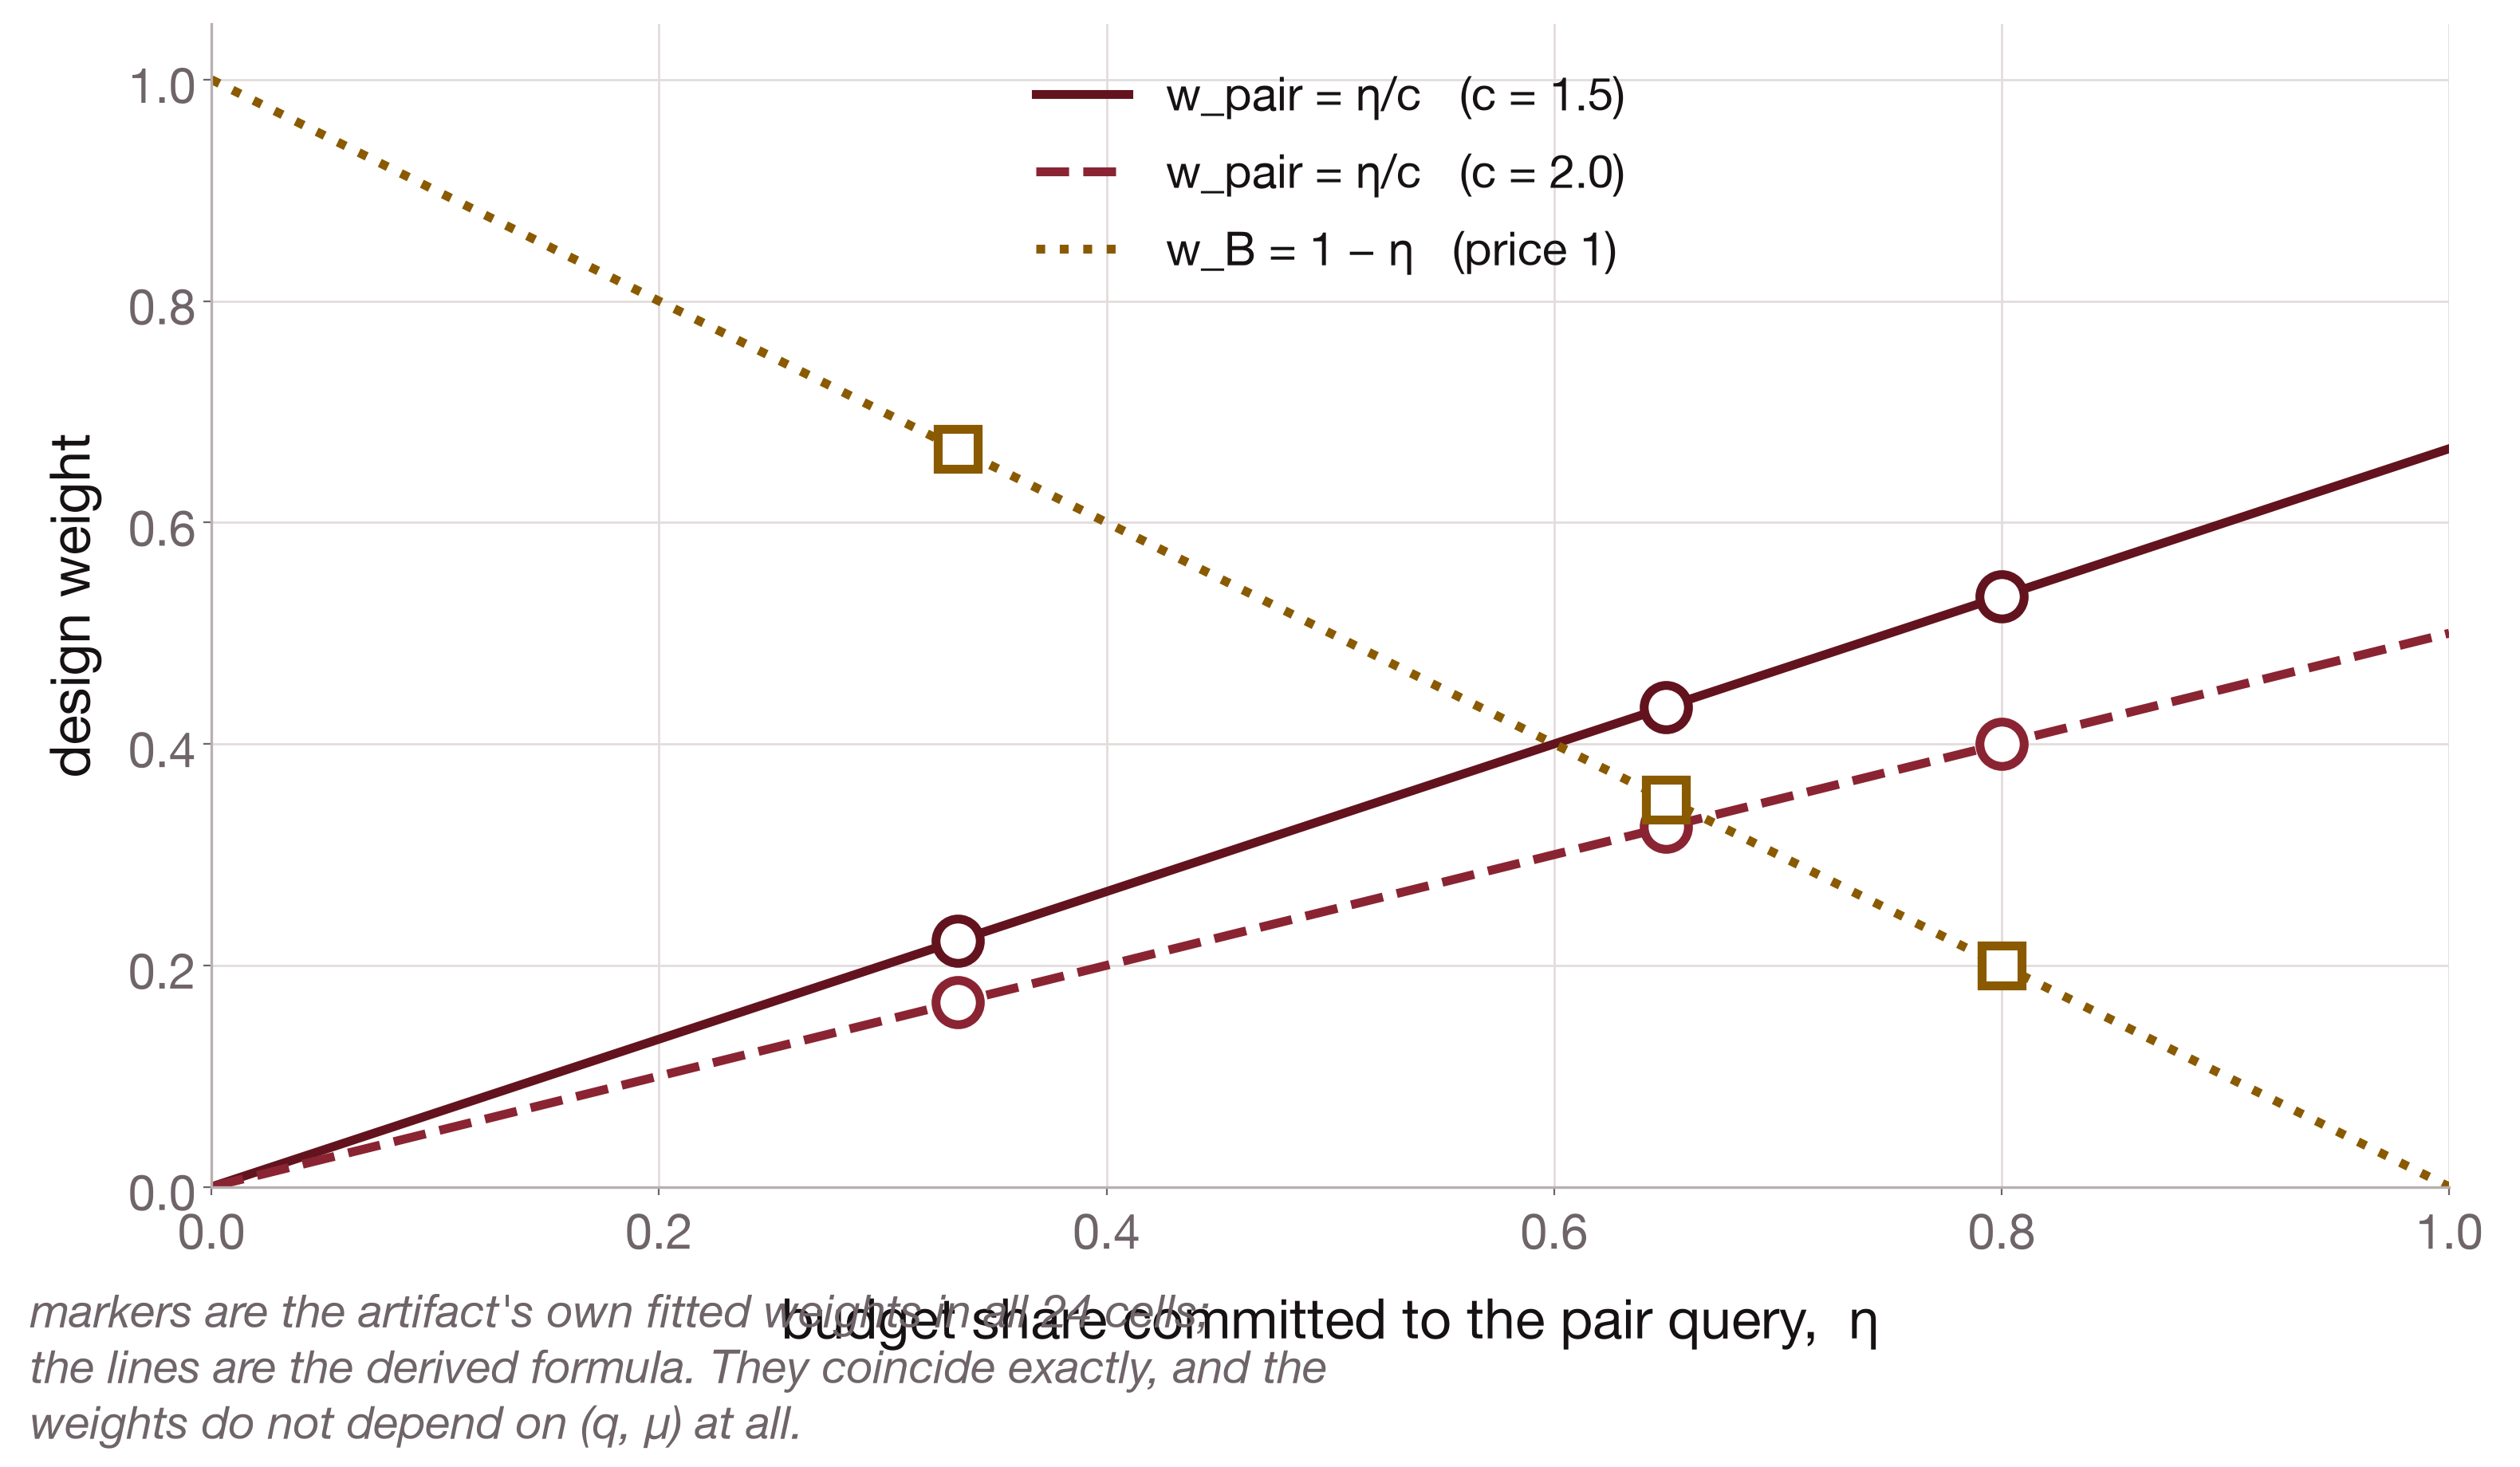
\includegraphics[width=\columnwidth]{d6_fig1_design.png}
\caption{Derived weights against the budget split. The lines are the formula
\eqref{eq:design}; the markers are the artifact's own fitted weights in all $24$ cells. They
coincide exactly, and as Corollary~\ref{cor:indep} predicts the weights do not depend on
$(q,\mu)$, so each marker stands for several cells differing in $(q,\mu)$.}
\label{fig:design}
\end{figure}

\subsection{The Margin-Sensitive Exchange Law}
\label{sec:margin}

The results so far concern the alternative family and the design. A sharper object is
available from the same development: an exchange bound in which the \emph{margin} between
selected and unselected coordinates appears explicitly.

\begin{lemma}[Score surplus from a common margin]
\label{lem:surplus}
Let $A,B$ be finite with $|A|=|B|$ and suppose every element of $A$ beats every element of
$B$ by at least $\mu$ in $\mathrm{score}$. Then
\begin{equation}
|A|\,\mu\;\leq\;\sum_{i\in A}\mathrm{score}(i)-\sum_{j\in B}\mathrm{score}(j).
\label{eq:surplus}
\end{equation}
\end{lemma}

\begin{proof}
If $B$ is empty both sides vanish. Otherwise take $b\in B$ maximising $\mathrm{score}$ on
$B$. Summing $\mu+\mathrm{score}(b)\le\mathrm{score}(i)$ over $A$ gives
$|A|(\mu+\mathrm{score}(b))\le\sum_{A}\mathrm{score}$, and
$\sum_{B}\mathrm{score}\le|B|\mathrm{score}(b)=|A|\mathrm{score}(b)$; subtracting gives
\eqref{eq:surplus}.
\end{proof}

\leanbox{\lean{score\_surplus\_ge\_card\_mul\_margin} in
\lean{LeanD6MarginSensitiveExchangeV1}}

The lemma is pure finite combinatorics---no geometry, no design---and it is stated separately
because it is what converts a margin hypothesis into a quantity the exchange bound can
consume.

\begin{theorem}[Exchange bound retaining the surplus]
\label{thm:exchange}
With $T$ Top-$k$ by $\mathrm{osc}\circ Q$ and $|S|=k$, writing $A=T\setminus S$ and
$B=S\setminus T$,
\begin{equation}
L_{F}(T)-L_{F}(S)\;\leq\;|A|\,\delta
 \;-\;\frac{1}{2}\Bigl(\sum_{j\in A}\mathrm{osc}(Q_{j})-\sum_{j\in B}\mathrm{osc}(Q_{j})\Bigr).
\label{eq:exchangesurplus}
\end{equation}
\end{theorem}

\leanbox{\lean{pair\_loss\_le\_sdiff\_card\_sub\_score\_surplus} in
\lean{LeanD6MarginSensitiveExchangeV1}}

The bracketed term is the surplus. An earlier endpoint-patch argument dropped it and retained
only $|A|\delta$; because $T$ is Top-$k$ the surplus is non-negative, so
\eqref{eq:exchangesurplus} is never weaker and is strictly stronger whenever the selected
scores exceed the unselected ones.

\begin{theorem}[Margin-sensitive exchange]
\label{thm:marginexchange}
If in addition every selected coordinate beats every unselected one by at least $\mu$, then
\begin{equation}
2\bigl(L_{F}(T)-L_{F}(S)\bigr)\;\leq\;|T\setminus S|\;\bigl(2\delta-\mu\bigr).
\label{eq:marginexchange}
\end{equation}
\end{theorem}

\begin{proof}
Apply Theorem~\ref{thm:exchange}, then bound the surplus below by Lemma~\ref{lem:surplus}
with $\mathrm{score}=\mathrm{osc}\circ Q$, using $|T\setminus S|=|S\setminus T|$ which holds
because $|T|=|S|$.
\end{proof}

\leanbox{\lean{pair\_doubled\_loss\_le\_card\_mul\_two\_delta\_sub\_margin} in
\lean{LeanD6MarginSensitiveExchangeV1}}

\noindent\emph{Supporting results in \lean{LeanD6MarginSensitiveExchangeV1}.}~These are the exchange law. The surplus lemma is pure finite combinatorics with no geometry in it, and it is what converts a margin hypothesis into a quantity the exchange bound can consume. The two exchange statements are ordered so that the first retains the surplus the earlier endpoint-patch argument discarded, and the second bounds that surplus below by the margin. They are reproduced as the prover has them; a further $0$ audited declarations in this module are positivity checks and measurability side conditions and are not displayed.

\noindent\textbf{S\,5}\quad\lean{pair\_doubled\_loss\_le\_card\_mul\_two\_delta\_sub\_margin}
{\footnotesize\[ \begin{aligned}[t]
&\{ \mathit{n} : \mathbb{N} \},\; (\mathit{q} : \mathit{Fin} (\mathit{n} + 1) \to \mathit{U} \to \mathbb{R} ),\; (\mathit{F} : (\mathit{Fin} (\mathit{n} + 1) \to \mathit{U})\\
&\quad \to \mathbb{R} ),\; (\mathit{delta} \mathit{mu} : \mathbb{R} ),\; (\mathit{hWeight} : \forall \mathit{c}, 0 \leq\\
&\quad \mathit{jointWeight} \mathit{q} \mathit{c}),\; (\mathit{hNorm} : \textstyle\sum \mathit{c}, \mathit{jointWeight} \mathit{q} \mathit{c} = 1),\\
&\quad \; (\mathit{hDeltaNonneg} : 0 \leq \mathit{delta}),\; (\mathit{hdelta} : \forall (\mathit{i} : \mathit{Fin} (\mathit{n} + 1)) (\mathit{x} \mathit{c} :\\
&\quad \mathit{Fin} (\mathit{n} + 1) \to \mathit{U}), |\mathit{mixedDifference} \mathit{F} \mathit{i} \mathit{x} \mathit{c}| \leq \mathit{delta}),\\
&\quad \; (\mathit{selected} \mathit{competitor} : \mathit{Finset} (\mathit{Fin} (\mathit{n} + 1))),\; (\mathit{k} : \mathbb{N} ),\\
&\quad \; (\mathit{hTop} : \mathit{IsTopKByScore} (\mathbf{fun} \mathit{j} \mapsto \mathit{osc} (\mathit{productResponse} \mathit{q} \mathit{F} \mathit{j}))\\
&\quad \mathit{selected} \mathit{k}),\; (\mathit{hCompetitorCard} : \mathit{competitor}.\mathit{card} = \mathit{k}),\\
&\quad \; (\mathit{hMargin} : \forall \mathit{i} \in \mathit{selected}, \forall \mathit{j} \notin \mathit{selected}, \mathit{mu} + \mathit{osc} (\\
&\quad \mathit{productResponse} \mathit{q} \mathit{F} \mathit{j}) \leq \mathit{osc} (\mathit{productResponse} \mathit{q} \mathit{F} \mathit{i}))\\
\vdash\;&2 * (\mathit{productCompressionLoss} \mathit{F} (\mathit{productResponse} \mathit{q} \mathit{F}) \mathit{selected}\\
&\quad - \mathit{productCompressionLoss} \mathit{F} (\mathit{productResponse} \mathit{q} \mathit{F}) \mathit{competitor})\\
&\quad \leq ((\mathit{selected} \ \mathit{competitor}).\mathit{card} : \mathbb{R} ) * (2 * \mathit{delta} - \mathit{mu})
\end{aligned} \]}

\noindent\textbf{S\,6}\quad\lean{pair\_loss\_le\_sdiff\_card\_sub\_score\_surplus}
{\footnotesize\[ \begin{aligned}[t]
&\{ \mathit{n} : \mathbb{N} \},\; (\mathit{q} : \mathit{Fin} (\mathit{n} + 1) \to \mathit{U} \to \mathbb{R} ),\; (\mathit{F} : (\mathit{Fin} (\mathit{n} + 1) \to \mathit{U})\\
&\quad \to \mathbb{R} ),\; (\mathit{delta} : \mathbb{R} ),\; (\mathit{hWeight} : \forall \mathit{c}, 0 \leq \mathit{jointWeight} \mathit{q} \mathit{c}),\\
&\quad \; (\mathit{hNorm} : \textstyle\sum \mathit{c}, \mathit{jointWeight} \mathit{q} \mathit{c} = 1),\; (\mathit{hDeltaNonneg} : 0 \leq\\
&\quad \mathit{delta}),\; (\mathit{hdelta} : \forall (\mathit{i} : \mathit{Fin} (\mathit{n} + 1)) (\mathit{x} \mathit{c} : \mathit{Fin} (\mathit{n} + 1) \to \mathit{U}),\\
&\quad |\mathit{mixedDifference} \mathit{F} \mathit{i} \mathit{x} \mathit{c}| \leq \mathit{delta}),\; (\mathit{selected} \mathit{competitor} :\\
&\quad \mathit{Finset} (\mathit{Fin} (\mathit{n} + 1))),\; (\mathit{k} : \mathbb{N} ),\; (\mathit{hTop} : \mathit{IsTopKByScore} (\mathbf{fun} \mathit{j}\\
&\quad \mapsto \mathit{osc} (\mathit{productResponse} \mathit{q} \mathit{F} \mathit{j})) \mathit{selected} \mathit{k}),\; (\mathit{hCompetitorCard}\\
&\quad : \mathit{competitor}.\mathit{card} = \mathit{k})\\
\vdash\;&\mathit{productCompressionLoss} \mathit{F} (\mathit{productResponse} \mathit{q} \mathit{F}) \mathit{selected} -\\
&\quad \mathit{productCompressionLoss} \mathit{F} (\mathit{productResponse} \mathit{q} \mathit{F}) \mathit{competitor} \leq\\
&\quad ((\mathit{selected} \ \mathit{competitor}).\mathit{card} : \mathbb{R} ) * \mathit{delta} - ((\mathit{selected}\\
&\quad \ \mathit{competitor}).\mathit{sum} (\mathbf{fun} \mathit{j} \mapsto \mathit{osc} (\mathit{productResponse} \mathit{q} \mathit{F} \mathit{j})) - (\\
&\quad \mathit{competitor} \ \mathit{selected}).\mathit{sum} (\mathbf{fun} \mathit{j} \mapsto \mathit{osc} (\mathit{productResponse} \mathit{q} \mathit{F} \mathit{j}))\\
&\quad ) / 2
\end{aligned} \]}

\noindent\textbf{S\,7}\quad\lean{score\_surplus\_ge\_card\_mul\_margin}
{\footnotesize\[ \begin{aligned}[t]
&\{ \mathit{I} : \mathit{Type}*\},\; [\mathit{DecidableEq} \mathit{I}],\; (\mathit{A} \mathit{B} : \mathit{Finset} \mathit{I}),\\
&\quad \; (\mathit{score} : \mathit{I} \to \mathbb{R} ),\; (\mathit{mu} : \mathbb{R} ),\; (\mathit{hCard} : \mathit{A}.\mathit{card} = \mathit{B}.\mathit{card}),\\
&\quad \; (\mathit{hMargin} : \forall \mathit{i} \in \mathit{A}, \forall \mathit{j} \in \mathit{B}, \mathit{mu} + \mathit{score} \mathit{j} \leq \mathit{score} \mathit{i})\\
\vdash\;&(\mathit{A}.\mathit{card} : \mathbb{R} ) * \mathit{mu} \leq \mathit{A}.\mathit{sum} \mathit{score} - \mathit{B}.\mathit{sum} \mathit{score}
\end{aligned} \]}


No symmetry is assumed, no active cell is fixed, and the reference is an arbitrary product
reference. The improvement over the $\delta$-only form is exactly $|T\setminus S|\mu$, which
is what makes the next subsection possible.

\subsection{The Sharp Threshold at Margin $2\delta$}
\label{sec:threshold}

Equation \eqref{eq:marginexchange} has an immediate consequence: at margin $2\delta$ the
right-hand side turns non-positive.

\begin{theorem}[Sufficiency]
\label{thm:sufficient}
If $2\delta\leq\rho$ then $L_{F}(T)\leq L_{F}(S)$ for every $S$ with $|S|=k$.
\end{theorem}

\begin{proof}
By Theorem~\ref{thm:marginexchange} the doubled difference is at most
$|T\setminus S|(2\delta-\rho)\le0$.
\end{proof}

\leanbox{\lean{margin\_two\_sufficient} in \lean{LeanD6SharpMarginThresholdV1}}

Theorem~\ref{thm:sufficient} holds for \emph{every} product reference, including degenerate
ones, because its proof uses only the mixed-difference bound and the weight axioms. That
matters because the matching necessity result does not.

\begin{theorem}[The steering construction attains the bound exactly]
\label{thm:steered}
For $A$ a coordinate set, $j\notin A$, $1\le\rho$, with $|A^{\complement}|=|A|$ and at least
two coordinates outside $A\cup\{j\}$, under the corner reference
\begin{equation}
2\bigl(L(A)-L(A^{\complement})\bigr)\;=\;|A|\,(2-\rho).
\label{eq:steered}
\end{equation}
\end{theorem}

\leanbox{\lean{steered\_exchange\_equality} in \lean{LeanD6SharpMarginThresholdV1}}

\begin{theorem}[Every sub-threshold margin fails]
\label{thm:subthreshold}
For $A$ non-empty and every $\rho\in[1,2)$, $A$ is Top-$k$ by the oscillation score and yet
$L(A^{\complement})<L(A)$.
\end{theorem}

\begin{proof}
$A$ is Top-$k$ by construction, and by \eqref{eq:steered} the doubled difference equals
$|A|(2-\rho)>0$.
\end{proof}

\leanbox{\lean{every\_subthreshold\_margin\_fails} in
\lean{LeanD6SharpMarginThresholdV1}}

\noindent\emph{Supporting results in \lean{LeanD6SharpMarginThresholdV1}.}~These are the threshold. Sufficiency is proved for an arbitrary product reference, including degenerate ones, because its proof uses only the mixed-difference bound and the weight axioms. The equality statement and the sub-threshold failure are both under the corner reference, which is the asymmetry Section~\ref{sec:discussion} reports and the reference sweep of Section~\ref{sec:results} quantifies. They are reproduced as the prover has them; a further $0$ audited declarations in this module are positivity checks and measurability side conditions and are not displayed.

\noindent\textbf{S\,8}\quad\lean{every\_subthreshold\_margin\_fails}
{\footnotesize\[ \begin{aligned}[t]
&\{ \mathit{n} : \mathbb{N} \},\; (\mathit{A} : \mathit{Finset} (\mathit{I} \mathit{n})),\; (\mathit{j} : \mathit{I} \mathit{n}),\; (\mathit{hj} : \mathit{j} \notin \mathit{A}),\\
&\quad \; (\mathit{hne} : \mathit{A}.\mathit{Nonempty}),\; (\mathit{rho} : \mathbb{R} ),\; (\mathit{hr} : 1 \leq \mathit{rho}),\\
&\quad \; (\mathit{hr2} : \mathit{rho} < 2),\; (\mathit{hbal} : \mathit{Aᶜ}.\mathit{card}=\mathit{A}.\mathit{card}),\\
&\quad \; (\mathit{hB} : 2 \leq (\mathit{others} \mathit{A} \mathit{j}).\mathit{card})\\
\vdash\;&\mathit{IsTopKByScore} (\mathbf{fun} \mathit{i} => \mathit{osc} (\mathit{productResponse} \mathit{corner} (\mathit{steered}\\
&\quad \mathit{A} \mathit{j} \mathit{rho}) \mathit{i})) \mathit{A} \mathit{A}.\mathit{card} \wedge \mathit{productCompressionLoss} (\mathit{steered} \mathit{A} \mathit{j} \mathit{rho}) (\\
&\quad \mathit{productResponse} \mathit{corner} (\mathit{steered} \mathit{A} \mathit{j} \mathit{rho})) \mathit{Aᶜ} <\\
&\quad \mathit{productCompressionLoss} (\mathit{steered} \mathit{A} \mathit{j} \mathit{rho}) (\mathit{productResponse}\\
&\quad \mathit{corner} (\mathit{steered} \mathit{A} \mathit{j} \mathit{rho})) \mathit{A}
\end{aligned} \]}

\noindent\textbf{S\,9}\quad\lean{margin\_two\_sufficient}
{\footnotesize\[ \begin{aligned}[t]
&\{ \mathit{U} : \mathit{Type}*\},\; [\mathit{Fintype} \mathit{U}],\; [\mathit{Nonempty} \mathit{U}],\; \{ \mathit{n} : \mathbb{N} \},\; (\mathit{q} : \mathit{I} \mathit{n} \to\\
&\quad \mathit{U} \to \mathbb{R} ),\; (\mathit{F} : (\mathit{I} \mathit{n} \to \mathit{U}) \to \mathbb{R} ),\; (\mathit{delta} \mathit{rho} : \mathbb{R} ),\\
&\quad \; (\mathit{hWeight} : \forall \mathit{c},0 \leq \mathit{jointWeight} \mathit{q} \mathit{c}),\; (\mathit{hNorm} : \textstyle\sum \mathit{c},\\
&\quad \mathit{jointWeight} \mathit{q} \mathit{c}=1),\; (\mathit{hd} : 0 \leq \mathit{delta}),\; (\mathit{hdelta} : \forall \mathit{i} \mathit{x} \mathit{c},\\
&\quad |\mathit{mixedDifference} \mathit{F} \mathit{i} \mathit{x} \mathit{c}| \leq \mathit{delta}),\; (\mathit{T} : \mathit{Finset} (\mathit{I} \mathit{n})),\\
&\quad \; (\mathit{k} : \mathbb{N} ),\; (\mathit{htop} : \mathit{IsTopKByScore} (\mathbf{fun} \mathit{i} => \mathit{osc} (\\
&\quad \mathit{productResponse} \mathit{q} \mathit{F} \mathit{i})) \mathit{T} \mathit{k}),\; (\mathit{hmargin} : \forall \mathit{i} \in \mathit{T},\forall \mathit{j} \notin \mathit{T},\\
&\quad \mathit{rho}+\mathit{osc} (\mathit{productResponse} \mathit{q} \mathit{F} \mathit{j}) \leq \mathit{osc} (\mathit{productResponse} \mathit{q} \mathit{F} \mathit{i})\\
&\quad ),\; (\mathit{hrho} : 2*\mathit{delta} \leq \mathit{rho}),\; (\mathit{S} : \mathit{Finset} (\mathit{I} \mathit{n})),\\
&\quad \; (\mathit{hS} : \mathit{S}.\mathit{card}=\mathit{k})\\
\vdash\;&\mathit{productCompressionLoss} \mathit{F} (\mathit{productResponse} \mathit{q} \mathit{F}) \mathit{T} \leq\\
&\quad \mathit{productCompressionLoss} \mathit{F} (\mathit{productResponse} \mathit{q} \mathit{F}) \mathit{S}
\end{aligned} \]}

\noindent\textbf{S\,10}\quad\lean{steered\_exchange\_equality}
{\footnotesize\[ \begin{aligned}[t]
&\{ \mathit{n} : \mathbb{N} \},\; (\mathit{A} : \mathit{Finset} (\mathit{I} \mathit{n})),\; (\mathit{j} : \mathit{I} \mathit{n}),\; (\mathit{hj} : \mathit{j} \notin \mathit{A}),\; (\mathit{rho} : \mathbb{R} ),\\
&\quad \; (\mathit{hr} : 1 \leq \mathit{rho}),\; (\mathit{hbal} : \mathit{Aᶜ}.\mathit{card}=\mathit{A}.\mathit{card}),\\
&\quad \; (\mathit{hB} : 2 \leq (\mathit{others} \mathit{A} \mathit{j}).\mathit{card})\\
\vdash\;&2*(\mathit{productCompressionLoss} (\mathit{steered} \mathit{A} \mathit{j} \mathit{rho}) (\mathit{productResponse}\\
&\quad \mathit{corner} (\mathit{steered} \mathit{A} \mathit{j} \mathit{rho})) \mathit{A}- \mathit{productCompressionLoss} (\mathit{steered} \mathit{A} \mathit{j}\\
&\quad \mathit{rho}) (\mathit{productResponse} \mathit{corner} (\mathit{steered} \mathit{A} \mathit{j} \mathit{rho})) \mathit{Aᶜ})=\\
&\quad (\mathit{A}.\mathit{card}:\mathbb{R} )*(2-\mathit{rho})
\end{aligned} \]}


Together these make the condition $\rho\ge2\delta$ sharp at $\delta=1$: sufficient for
Top-$C$ optimality, and violated for every $\rho$ in $[1,2)$.

Three scope statements belong here rather than in the Discussion, because the result invites
over-reading. It is a Top-$C$ optimality threshold, not a minimax value: it says when the
Top-$C$ rule is optimal among same-cardinality sets, and says nothing about the minimax value
of the whole same-response fibre, which is a different quantifier and is open. Sufficiency and
necessity do not share a reference class, as noted above. And robustness to the reference
was measured rather than assumed: an exact rational sweep of the product reference
$q_{i}(1)=t$, reported in Section~\ref{sec:results}, finds that the witness does not collapse
the moment the corner is left but degrades continuously, and fails only past a breakdown point
$t^{\star}(\mu)$ that grows with the margin and is never reached at $\mu=2$. The mechanism is
that the steered coordinate $j$ accumulates span as the reference acquires interior mass, so
the separation the corner enforces between $A$ and its complement narrows until $j$ overtakes
$A$ on score and $A$ is no longer the Top-$C$ set.

\begin{figure}[htbp]
\centering
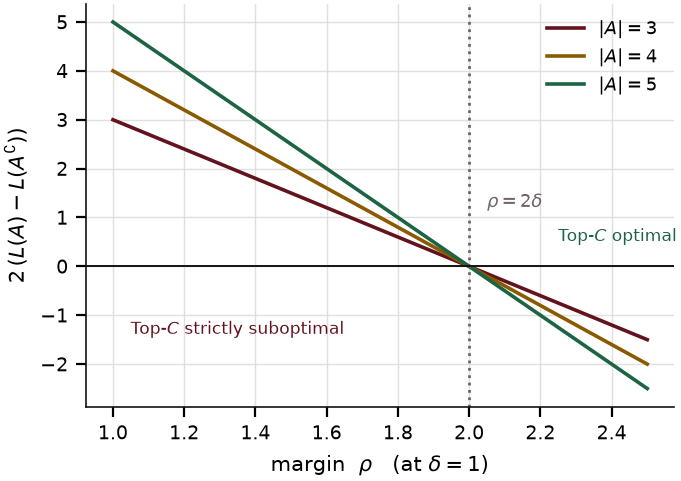
\includegraphics[width=\columnwidth]{d6_fig3_threshold.png}
\caption{The exchange law of \lean{steered\_exchange\_equality}, drawn at $\delta=1$. The
doubled regret of the Top-$C$ set against its complement is exactly $|A|(2-\rho)$: positive
below the threshold $\rho=2\delta$, where the construction of
Theorem~\ref{thm:subthreshold} makes Top-$C$ strictly worse than a same-cardinality
competitor, and non-positive at and above it, where Theorem~\ref{thm:sufficient} forbids any
competitor from beating it. The two theorems meet at $\rho=2$ with no gap between them, which
is what makes the threshold sharp rather than merely bracketed. The lines are the proved
identity evaluated, not a fit, and the slope $-|A|$ is why a larger selected set is penalised
more by the same margin deficit.}
\label{fig:threshold}
\end{figure}

\subsection{The Separation Certificate on a Cell}
\label{sec:certificate}

A separate question is whether a claimed strict separation survives across a whole parameter
cell rather than at sampled points.

\begin{lemma}[Quadratic infimum on an interval]
\label{lem:quadinf}
For $f(x)=ax^{2}+bx+c$ with $a\ge0$ on $[l,u]$,
$\inf_{[l,u]}f=\min\{f(l),f(u),f(x^{\dagger})\}$ with $x^{\dagger}=-b/2a$ when $a>0$ and
$x^{\dagger}\in[l,u]$.
\end{lemma}

\leanbox{\lean{quadratic\_inf\_Icc} in \lean{LeanD6AlternativeReductionV1}}

\begin{theorem}[Separation across a cell]
\label{thm:modulus}
On a cell $[t_{0},t_{1}]$, if
\begin{equation}
L_{\mathrm{full}}(t_{0})\;>\;\rho_{\mathrm{two}}\;U_{\mathrm{two}}(t_{0}),
\qquad \rho\;=\;r^{(t_{1}-t_{0})/q},
\label{eq:modulus}
\end{equation}
then the strict separation holds throughout the cell.
\end{theorem}

\leanbox{\lean{no\_crossing\_of\_modulus}, \lean{crossing\_bracket} in
\lean{LeanD6AlternativeReductionV1}}

\noindent\emph{Supporting results in \lean{LeanD6AlternativeReductionV1}.}~These are the certificate machinery. The quadratic infimum is given at the vertex and at each endpoint separately, which is what reduces a continuous range of $x$ to three evaluations; the crossing statements then propagate the verdict across a cell by an exact multiplicative factor rather than by sampling within it. They are reproduced as the prover has them; a further $4$ audited declarations in this module are positivity checks and measurability side conditions and are not displayed.

\noindent\textbf{S\,11}\quad\lean{crossing\_bracket}
{\footnotesize\[ \begin{aligned}[t]
&(\mathit{f} : \mathbb{R} \to \mathbb{R} ),\; (\mathit{t0} \mathit{t1} : \mathbb{R} ),\; (\mathit{ht} : \mathit{t0} \leq \mathit{t1}),\; (\mathit{hc} :\\
&\quad \mathit{ContinuousOn} \mathit{f} (\mathit{Set}.\mathit{Icc} \mathit{t0} \mathit{t1})),\; (\mathit{h0} : \mathit{f} \mathit{t0} \leq 0),\; (\mathit{h1} : 0 \leq \mathit{f} \mathit{t1})\\
\vdash\;&\exists \mathit{t} \in \mathit{Set}.\mathit{Icc} \mathit{t0} \mathit{t1}, \mathit{f} \mathit{t} = 0
\end{aligned} \]}

\noindent\textbf{S\,12}\quad\lean{no\_crossing\_of\_modulus}
{\footnotesize\[ \begin{aligned}[t]
&(\mathit{f} : \mathbb{R} \to \mathbb{R} ),\; (\mathit{t0} \mathit{t1} \mathit{Lip} \mathit{m} : \mathbb{R} ),\; (\mathit{ht} : \mathit{t0} \leq \mathit{t1}),\\
&\quad \; (\mathit{hLip} : 0 \leq \mathit{Lip}),\; (\mathit{hlip} : \forall \mathit{s} \in \mathit{Set}.\mathit{Icc} \mathit{t0} \mathit{t1}, |\mathit{f} \mathit{s} - \mathit{f} \mathit{t0}| \leq\\
&\quad \mathit{Lip} * (\mathit{s} - \mathit{t0})),\; (\mathit{hm} : \mathit{m} \leq \mathit{f} \mathit{t0}),\; (\mathit{hpos} : 0 < \mathit{m}),\\
&\quad \; (\mathit{hgap} : \mathit{Lip} * (\mathit{t1} - \mathit{t0}) < \mathit{m})\\
\vdash\;&\forall \mathit{t} \in \mathit{Set}.\mathit{Icc} \mathit{t0} \mathit{t1}, 0 < \mathit{f} \mathit{t}
\end{aligned} \]}

\noindent\textbf{S\,13}\quad\lean{quadratic\_inf\_attained}
{\footnotesize\[ \begin{aligned}[t]
&(\mathit{a} \mathit{b} \mathit{c} \mathit{lo} \mathit{hi} : \mathbb{R} ),\; (\mathit{ha} : 0 < \mathit{a}),\; (\mathit{hv1} : \mathit{lo} \leq -\mathit{b} / (2 * \mathit{a})),\\
&\quad \; (\mathit{hv2} : -\mathit{b} / (2 * \mathit{a}) \leq \mathit{hi})\\
\vdash\;&(\forall \mathit{x}, \mathit{lo} \leq \mathit{x} \to \mathit{x} \leq \mathit{hi} \to \mathit{a} * (-\mathit{b} / (2 * \mathit{a})) ^{2} + \mathit{b} * (-\mathit{b} / (\\
&\quad 2 * \mathit{a})) + \mathit{c} \leq \mathit{a} * \mathit{x} ^{2} + \mathit{b} * \mathit{x} + \mathit{c}) \wedge \mathit{lo} \leq -\mathit{b} / (2 * \mathit{a}) \wedge\\
&\quad -\mathit{b} / (2 * \mathit{a}) \leq \mathit{hi}
\end{aligned} \]}


The information \eqref{eq:ib} is quadratic in $x$ with non-negative leading coefficient, so
Lemma~\ref{lem:quadinf} reduces a continuous $x$-range to three evaluations. Both verdicts use
outward \emph{rational} enclosures and exact gaps rather than floating point, so a certificate
is a proof about the cell and not a statement about the points sampled in it.

\begin{figure}[htbp]
\centering
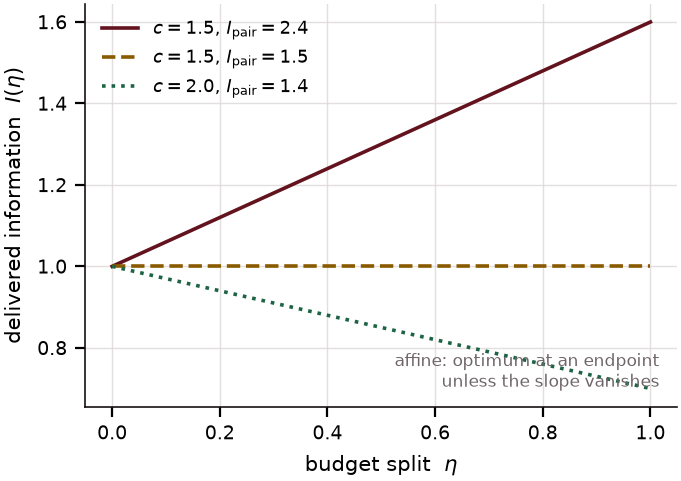
\includegraphics[width=\columnwidth]{d6_fig4_affine.png}
\caption{Why the optimal design is pure except on a threshold. Theorem~\ref{thm:affine} makes
delivered information affine in the budget split $\eta$, so $I(\eta)$ is a straight line
between $I_{B}$ at $\eta=0$ and $I_{\mathrm{pair}}/c$ at $\eta=1$, whatever the parameters.
An affine function on an interval attains its maximum at an endpoint unless its slope is
zero, so the optimum is pure---all budget to one query type---except on the single surface
$I_{\mathrm{pair}}=c\,I_{B}$ where the line is flat and every split is optimal. The three
lines show the two strict cases and the degenerate one. Exact evaluation of
\eqref{eq:transitioncond}.}
\label{fig:affine}
\end{figure}

\section{Experimental Design}
\label{sec:expdesign}

\subsection{Experimental Objectives}

The theorems quantify over all parameters, so the numerical work cannot strengthen them. It
has two objectives. The first is to confirm that the derived weights agree with the previously
fitted ones on the cells where the fit was performed, which is a check on the implementation.
The second concerns a hypothesis rather than an implementation. The sufficiency half of the
threshold, Theorem~\ref{thm:sufficient}, is proved for an arbitrary product reference; the
necessity half, Theorem~\ref{thm:subthreshold}, is proved at the corner reference only.
Nothing in the formal development says what happens between them, and the honest question is
not whether the witness survives an arbitrary reference---it is not claimed to---but how far
from the corner it survives, and whether the failure is abrupt or gradual. Experiment~E2
measures that.

\subsection{Setup}

The design grid is $q\in\{8,16\}$, $\mu\in\{\tfrac14,\tfrac25\}$, $c\in\{\tfrac32,2\}$ and
$\eta\in\{\tfrac13,\tfrac{13}{20},\tfrac45\}$, giving $24$ cells. The separation certificate
is evaluated on eight cells, and the pair-query necessity test on twenty.

\subsection{E2: The Reference Sweep}
\label{sec:e2}

The reference is moved off the corner along the one-parameter product family
$q_{i}(\mathrm{true})=t$, which places mass $t$ on the true response in every coordinate
independently and recovers the corner at $t=0$. The grid is the seventeen rationals
$t=0,\tfrac1{32},\dots,\tfrac12$, crossed with two dimensions $n\in\{6,8\}$ and five margins
$\rho\in\{1,\tfrac54,\tfrac32,\tfrac74,2\}$---one hundred and seventy cells, of which one
hundred and sixty have $t>0$.

\begin{algorithm}[htbp]
\caption{Evaluating the construction under one reference}
\label{alg:sweep}
\begin{algorithmic}[1]
\REQUIRE dimension $n$, selected set $A$, steered coordinate $j\notin A$, margin $\mu$,
         product reference $q_{i}(\mathrm{true})=t_{i}$
\ENSURE whether $A$ is still a Top-$C$ set, and the doubled regret against its complement
\STATE $F(x)\leftarrow\textsc{Steered}(A,j,\mu)(x)$ for every $x\in\{0,1\}^{n}$
       \COMMENT{independent of the reference, so tabulated once per configuration and
       reused across every $t$ --- this is what makes the wide sweep affordable}
\STATE $W(c)\leftarrow\prod_{i}\bigl(t_{i}\text{ if }c_{i}\text{ else }1-t_{i}\bigr)$
\FORALL{coordinates $i$ and values $u\in\{0,1\}$}
  \STATE $Q_{i}(u)\leftarrow\sum_{c}W(c)\,F(c\text{ with }c_{i}:=u)$
\ENDFOR
\STATE $\mathrm{osc}_{i}\leftarrow|Q_{i}(1)-Q_{i}(0)|$;
       $\;T\leftarrow$ the $|A|$ coordinates of largest $\mathrm{osc}$
\STATE $L(S)\leftarrow\tfrac12\bigl(\max_{x}-\min_{x}\bigr)
       \bigl[F(x)-\sum_{i\in S}Q_{i}(x_{i})\bigr]$
\RETURN $\bigl[T=A\bigr]$ and $2\bigl(L(A)-L(A^{\complement})\bigr)$
\end{algorithmic}
\end{algorithm}

\noindent All of it is exact rational arithmetic, so a reported flip is a flip and not a
rounding artefact. Two properties of the setup matter more than its size. First, every quantity is computed in
exact rational arithmetic, so a reported flip is a flip and not a rounding artefact. Second,
the definitions are not re-derived for the experiment: the gate, the coefficient map, the
steered world and the compression loss are transcribed from the Lean sources, and the
transcription is validated before any sweep result is reported. At $t=0$ the transcription
must reproduce \lean{steered\_span}---oscillation $\rho$ on $A$ and $0$ off it---and
\lean{steered\_exchange\_equality}---doubled regret exactly $|A|(2-\rho)$. It does, in all
nine validation configurations and all ten corner cells. A sweep whose code does not
reproduce the theorems at the one point where the theorems apply is measuring something else,
and this check is what rules that out.

\subsection{E3: Four Axes Instead of One}
\label{sec:e3}

E2 moves the reference along a single symmetric path. That leaves the obvious objection
unanswered: the path is symmetric, the construction is symmetric, and a symmetric
perturbation may be the one direction in which nothing happens. E3 widens the sweep on four
axes at once.

\emph{Dimension.} $n\in\{6,8,10\}$ with $|A|=n/2$. The balance is not a convenience: the
exchange equality carries the hypothesis $|A^{\complement}|=|A|$, so these are the
configurations the theorems speak about. Twelve unbalanced configurations are swept as well,
in a separate arm, precisely because the theorem does not cover them---and nothing there is
checked against it.

\emph{Margin and resolution.} Nine margins from $1$ to $2$ rather than five, on a
sixty-five-point grid in $t$, so the breakdown point is located to $1/64$ and can be traced
against the margin rather than sampled.

\emph{Direction.} This is the axis that answers the objection. Besides the symmetric path,
four structured directions perturb only $A$, only its complement, only the steered coordinate
$j$, or everything but $j$; and two hundred references per configuration are drawn with an
independent $t_{i}$ in each coordinate. If the finding survives an asymmetric reference it is
not an artefact of the symmetric one.

Responses of the steered world do not depend on the reference, so they are tabulated once per
configuration and reused, which is what makes the wider sweep affordable. Both self-checks of
Section~\ref{sec:e2} are re-run at every configuration.

\subsection{Metrics}

For the design experiment: the two derived weights, the budget residual
$w_{B}+c\,w_{\mathrm{pair}}-1$, agreement with the fitted values, the certificate verdict per
cell and which endpoint produced it, and the number of cells in which the pair query carries
positive weight and its necessity is certified.

For E2, three quantities per cell: whether $A$ is still a Top-$C$ set under the perturbed
reference, which is the hypothesis of Theorem~\ref{thm:subthreshold}; the doubled regret
$2(L(A)-L(A^{\complement}))$, which is its conclusion; and the oscillation profile that
explains the two. Reporting the hypothesis and the conclusion separately is deliberate---they
fail at different values of $t$, and a single pass/fail per cell would hide that.

\subsection{Statistical Reporting}

Every quantity in this section is exact rational arithmetic; there is no sampling, no seed and
no confidence interval anywhere in it. E2 is labelled \NUM{} throughout, not because it is
inexact---it is exact---but because it is a finite sweep of a parameter family and supports no
universally quantified claim. No result from it is used to support a \PROVED{} one, and where
it bears on a proved statement, as at $t=0$, it is a check on the transcription rather than
evidence for the theorem.

\section{Formal Verification}
\label{sec:verification}

\subsection{Acceptance Contract}

A module counts as accepted only when all six of the following hold: the compiler exits zero
with no errors; the source hash is unchanged \emph{across} the compile, so the file checked is
the file on disk; the compiled artifact is newer than its source; at least one
\texttt{\#print axioms} directive is present; the axiom set of every audited declaration lies
within $\{\textsf{propext},\textsf{Classical.choice},\textsf{Quot.sound}\}$; and no
\texttt{sorry} appears anywhere in the file.

This contract is shared with the other papers of the programme and is reproduced verbatim in
each, so that no paper's evidence claim has to be read against a different standard; the
wording is common and the counts in this section are not. The contract is stated in full
because each clause excludes a specific way of appearing verified without being so. The hash check across the compile excludes editing a file after
checking it; the artifact-newer check excludes a stale \texttt{.olean}; and the axiom audit is
a \emph{whitelist} rather than a blacklist, so an axiom introduced by a decision procedure
outside the kernel is rejected by name mismatch rather than needing to be anticipated.

\subsection{Evidence per Step}

\begin{table}[htbp]
\caption{Evidence per step. All cited declarations are axiom-audited.}
\label{tab:inventory}
\centering\footnotesize\setlength{\tabcolsep}{3pt}
\begin{tabular}{@{}llr@{}}
\toprule
Step & Module & Aud. \\
\midrule
Slice, Thms~\ref{thm:slice}--\ref{thm:nonblind} & \lean{LeanD6GeneralFamilyV1}       & 5 \\
Design, Thms~\ref{thm:unique}--\ref{thm:affine} & \lean{LeanD6DesignDerivationV1}    & 7 \\
Surplus, Lem~\ref{lem:surplus}                  & \lean{LeanD6MarginSensitiveExchangeV1} & 3 \\
Exchange, Thms~\ref{thm:exchange}--\ref{thm:marginexchange} & \lean{LeanD6MarginSensitiveExchangeV1} & 3 \\
Threshold, Thms~\ref{thm:sufficient}--\ref{thm:subthreshold} & \lean{LeanD6SharpMarginThresholdV1} & 3 \\
Separation, Thm~\ref{thm:modulus}               & \lean{LeanD6AlternativeReductionV1} & 7 \\
\bottomrule
\end{tabular}
\end{table}

\subsection{Scope of the Formalisation}

The D6 strand contains $444$ Lean source files with $4{,}087$ theorem and lemma statements,
of which $30$ modules carry an acceptance receipt covering $187$ audited declarations. Across
the programme: $762$ files, $7{,}199$ statements, $111$ accepted modules, $857$ audited
declarations.

The ratio of strand size to displayed equations invites the question of what the rest is doing,
and the answer is characteristic. Most of the strand is search and refutation: establishing
that the $(d,x)$ family is the right one required first establishing that several other
candidate families were not, and each withdrawn formulation leaves behind the statements that
ruled it out. The separation certificates are issued per cell, so the file count scales with
the parameter grid rather than with mathematical content.
Every audited statement of every module this paper cites is displayed in Section~\ref{sec:setting}, attached to the step that uses it; only positivity checks and measurability side conditions are omitted, and their count is given at each block. The strand contains a further $26$ accepted modules carrying $167$ audited declarations that no step of this paper uses; they belong to other results of the programme. Appendix~\ref{app:inventory} reproduces the complete chain: all $187$ audited statements of the strand across its $30$ accepted modules, grouped by module.

\section{Results}
\label{sec:results}

\subsection{Reporting Protocol}

All $24$ cells are reported with no exclusions.

\subsection{The Derived Weights Match All 24 Cells Exactly}

The previously fitted weights agree with \eqref{eq:design} in every cell, and the budget
identity holds exactly in each. The weights vary with $(\eta,c)$ and are constant across
$(q,\mu)$, exactly as Corollary~\ref{cor:indep} predicts.

The logical status of the table changed with Section~\ref{sec:design}. Before the derivation
it was the evidence---$24$ consistent cells, suggestive but not conclusive, licensing no
prediction at a $25$th cell. After it, the table is a check on the arithmetic: the theorem
says the agreement must hold at every $(q,\mu,c,\eta)$, so a disagreeing cell would now be an
implementation bug rather than a puzzle.

\subsection{The Separation Is Certified on Every Cell Tested}

Eight of eight cells certify the strict separation across the whole cell, all by the
left-endpoint test of \eqref{eq:modulus}, with exact rational gaps. That every certificate
came from the same endpoint is itself informative: the modulus decays across the cell, so the
binding case is the left edge, and a procedure testing the midpoint would have been testing
the easy case.

\subsection{The Pair Query Is Necessary Wherever It Is Used}

On $20$ parameter cells the pair query carries positive weight in $17$, and in all $17$ its
necessity is certified: the full value strictly exceeds the best value achievable without it.
The three cells without a certificate are exactly those where the pair weight is zero. The
coincidence of those two sets is the point---a missing certificate indicates a cell where the
query is unused, not one where the argument failed.

\begin{figure}[htbp]
\centering
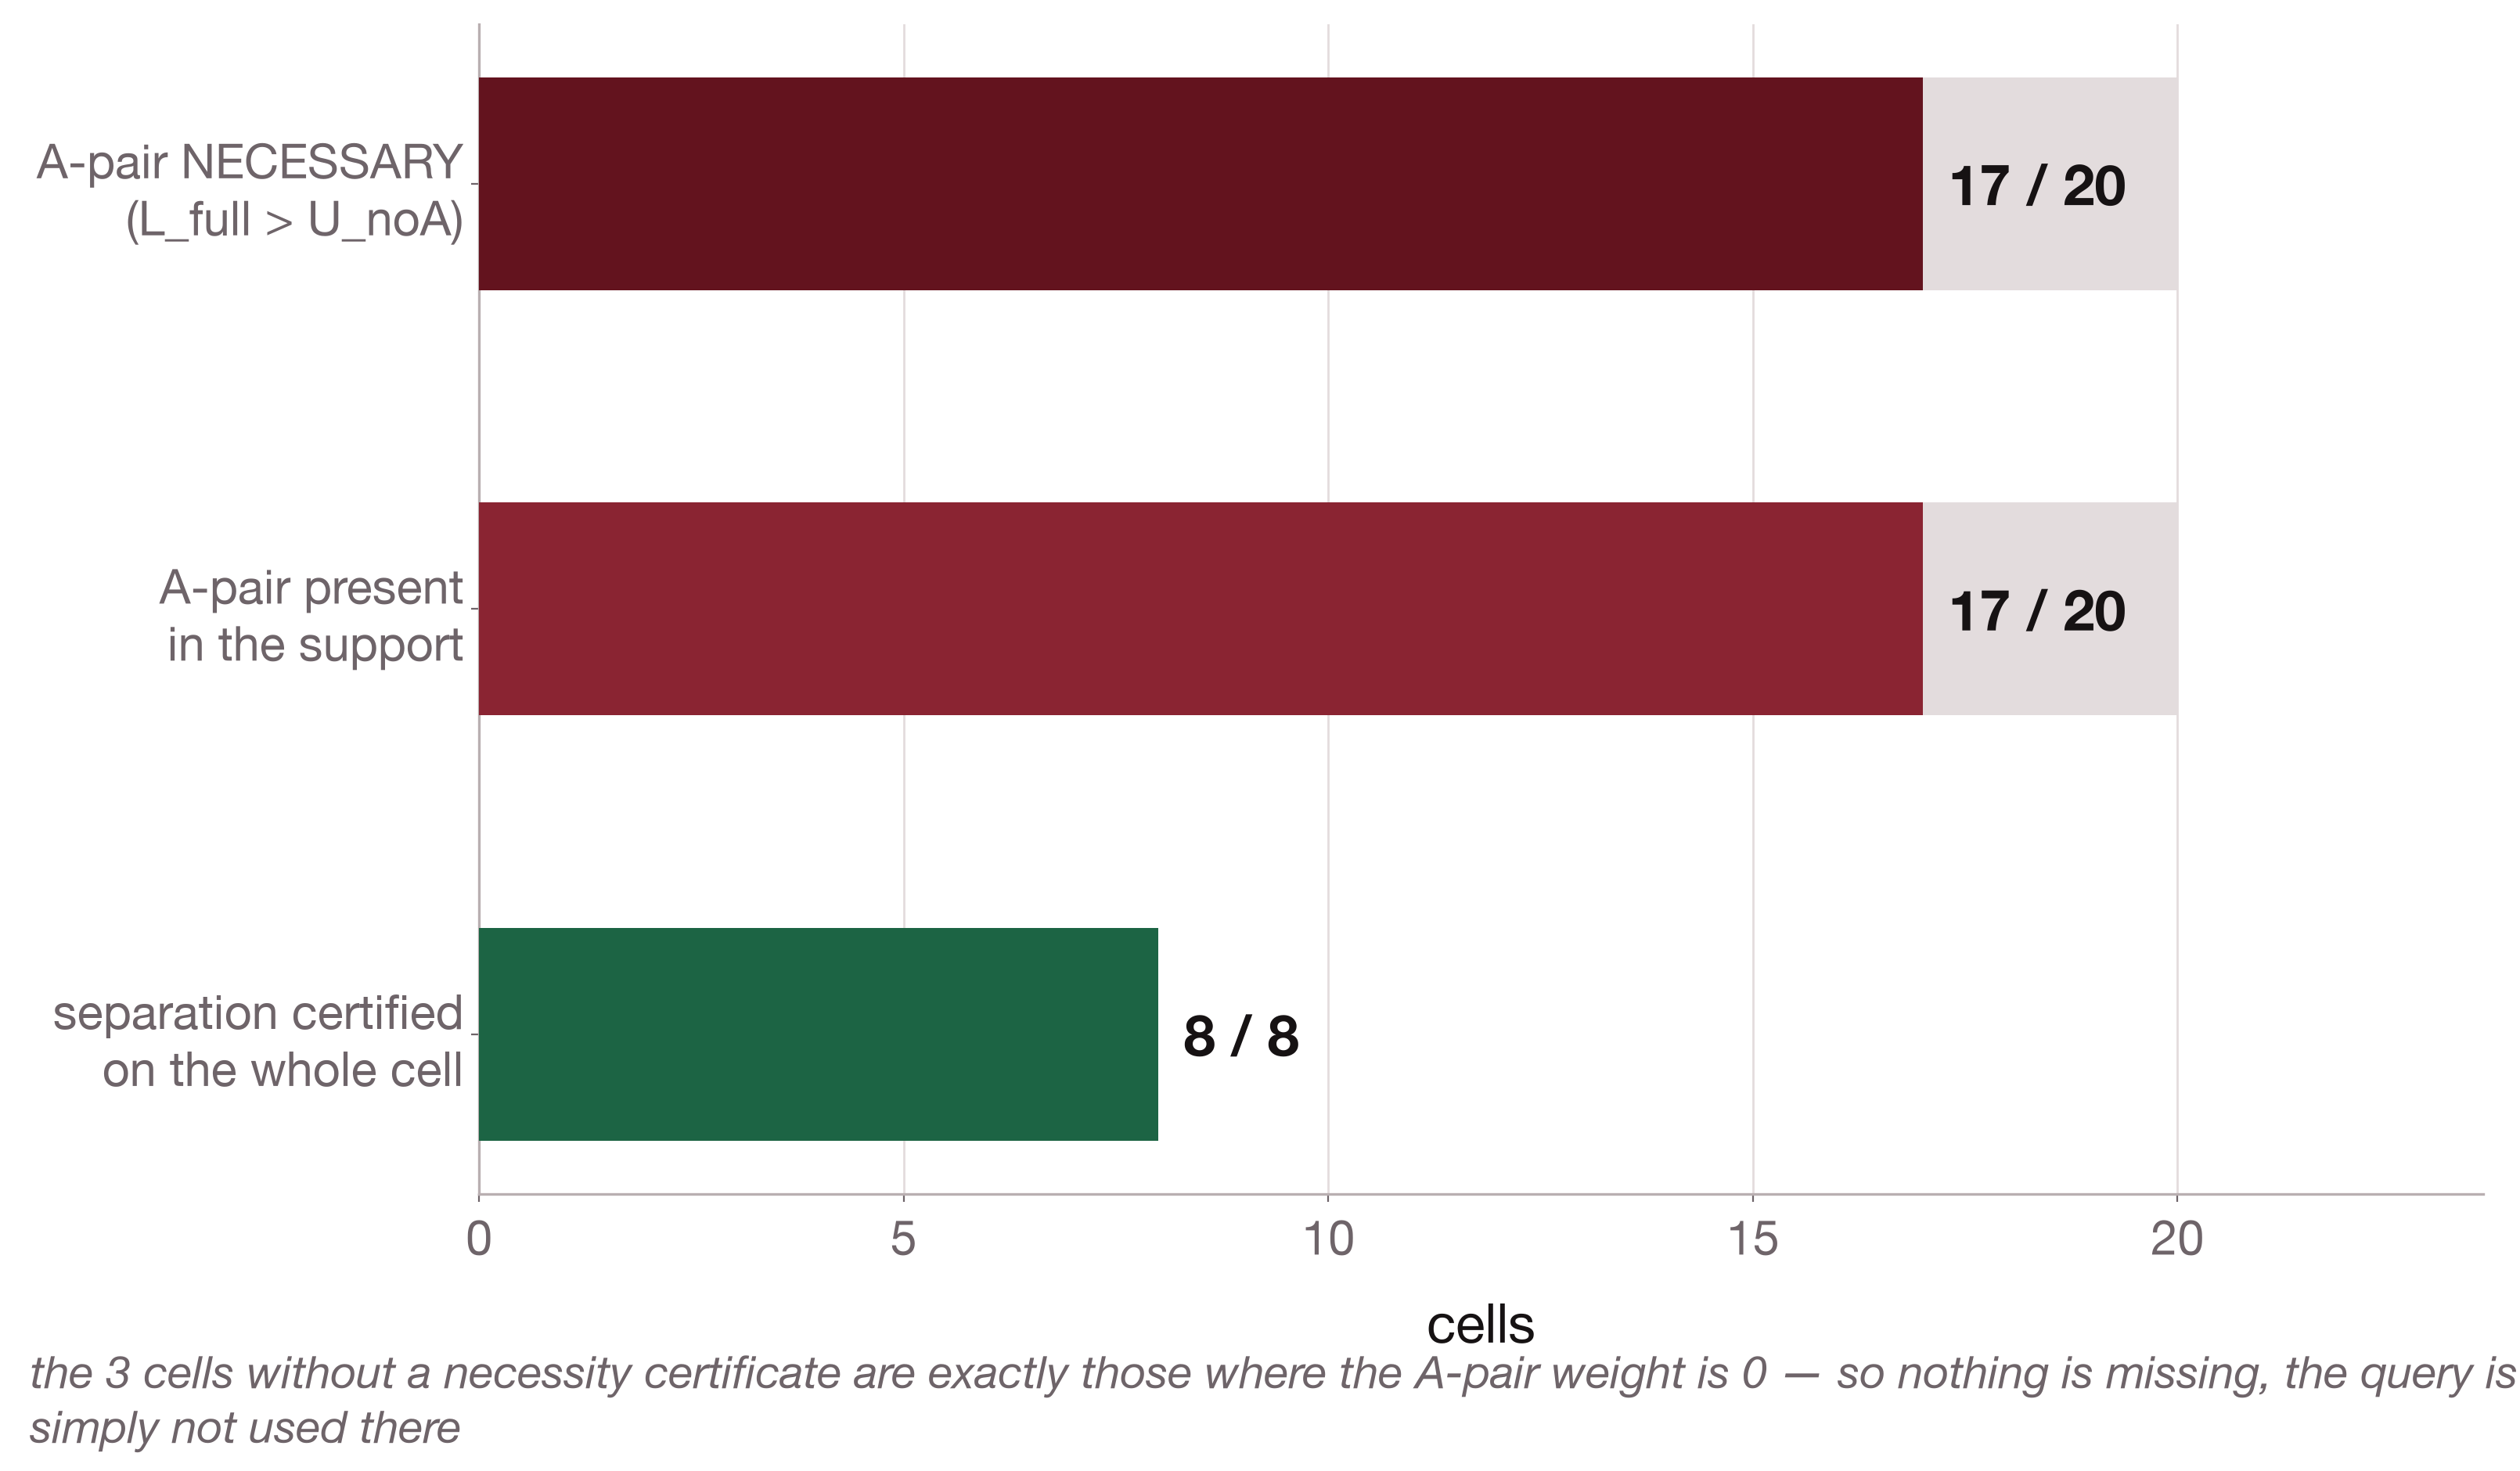
\includegraphics[width=\columnwidth]{d6_fig2_certificates.png}
\caption{Certificate counts. The three cells without a necessity certificate are exactly
those where the pair weight is zero.}
\label{fig:certificates}
\end{figure}

\subsection{How Far From the Corner the Witness Survives}
\label{sec:refsweep}

The sweep of Section~\ref{sec:e2} answers a question the theorems leave open, and the answer
is not the one the first draft of this paper assumed.

At $t=0$ the transcription reproduces both proved statements exactly: the oscillation profile
matches \lean{steered\_span} in all nine validation configurations, and the doubled regret
equals $|A|(2-\rho)$ in all ten corner cells, to the last bit of exact rational arithmetic.
The sweep is therefore measuring the construction the theorems describe.

Away from the corner the construction does not collapse. It degrades, continuously and
predictably. Figure~\ref{fig:reference} plots the doubled regret against $t$: every curve
leaves its corner value $|A|(2-\rho)$ smoothly and decreases monotonically, and no curve
drops discontinuously at any $t>0$. What does happen is that the two failure modes separate.
The hypothesis of Theorem~\ref{thm:subthreshold} fails first in some cells and second in
others. Its hypothesis is that $A$ is a Top-$C$ set; as $t$ grows, the steered coordinate $j$
accumulates oscillation---its span rises from $0$ at the corner to $0.91$ at $t=\tfrac12$ in
the $\rho=1$, $n=6$ cell, while the coordinates of $A$ fall from $1$ to $0.09$---until $j$
overtakes $A$ and the hypothesis is no longer met. Its conclusion is that the regret is
positive, which fails at a different $t$.

The breakdown point of the hypothesis rises with the margin, monotonically and in both
dimensions: at $n=6$ the first flip occurs at $t=\tfrac{7}{32},\tfrac{9}{32},\tfrac{11}{32}$
and $\tfrac{15}{32}$ for $\rho=1,\tfrac54,\tfrac32,\tfrac74$, and at $n=8$ at
$t=\tfrac{5}{32},\tfrac{7}{32},\tfrac{9}{32}$ and $\tfrac38$. Across the sweep $61$ of the
$160$ cells with $t>0$ lose the Top-$C$ property, a rate of $38.1\%$ that falls from $68.8\%$
at $\rho=1$ to $21.9\%$ at $\rho=\tfrac74$. Once a cell flips it stays flipped: the
transition is a single threshold in $t$, not an oscillation. \NUM{}

The $\rho=2$ column is the one to read last. At the threshold margin, $A$ remains a Top-$C$
set at every $t$ on the grid and the doubled regret is non-positive at every $t>0$---the
Top-$C$ set is never beaten. Theorem~\ref{thm:sufficient} is proved for an arbitrary product
reference, so the sweep cannot confirm it in the logical sense; what it does is exercise the
theorem on thirty-two references outside the corner where the necessity construction lives,
and find no violation. Sufficiency and necessity behave differently off the corner in exactly
the direction the proofs predict, which is weak evidence, but it is evidence about the part of
the parameter space no proof here covers.

The practical reading is narrower than the first draft of this paper claimed and broader than
the theorem states. Necessity is proved at $t=0$ and holds, measurably, in a neighbourhood
whose size grows with the margin; it is not a corner-only curiosity, and it is not a theorem
away from the corner either.

\begin{figure}[htbp]
\centering
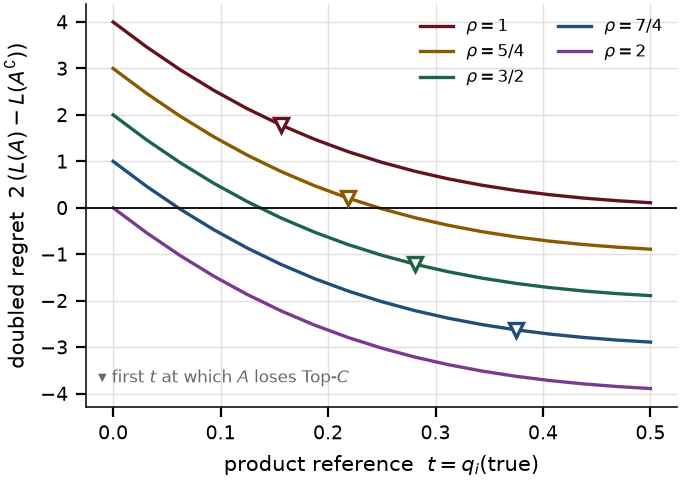
\includegraphics[width=\columnwidth]{d6_fig5_reference.png}
\caption{The necessity construction as the reference leaves the corner, at $n=8$. Each curve
is the doubled regret $2(L(A)-L(A^{\complement}))$ at one margin, in exact rational
arithmetic, against the product reference $q_{i}(\mathrm{true})=t$; at $t=0$ the five curves
begin at $|A|(2-\rho)=4,3,2,1,0$, which is \lean{steered\_exchange\_equality} reproduced by
the transcription rather than assumed by it. Triangles mark the first $t$ at which $A$ ceases
to be a Top-$C$ set, so the hypothesis of Theorem~\ref{thm:subthreshold} stops holding; they
move right as the margin grows and are absent at $\rho=2$, where the set stays Top-$C$
throughout and the regret is non-positive at every $t>0$. The construction degrades with the
reference; it does not fail at the first perturbation. \NUM{}}
\label{fig:reference}
\end{figure}

\subsection{The Finding Is Not an Artefact of the Symmetric Path}
\label{sec:e3results}

Three results from the wider sweep of Section~\ref{sec:e3}, in order of what they rule out.

\emph{The breakdown point is a real function of the margin.} At every one of the three sizes,
the first $t$ at which $A$ ceases to be the Top-$C$ set rises monotonically with the margin,
with no exception and no reversal: at $n=6$ it runs from $13/64$ at $\mu=1$ to $15/32$ at
$\mu=7/4$, at $n=8$ from $5/32$ to $7/16$, and at $n=10$ from $1/8$ to $23/64$.
Figure~\ref{fig:wide} plots all three. The curves also fall with $n$, so the construction
tolerates less perturbation as the space grows---which is worth knowing and which the
single-path sweep could only hint at from two points. The transition is a threshold, not an
oscillation: once a cell flips it stays flipped, at every configuration. \NUM{}

\emph{It is not the symmetric path.} Asymmetric references drawn with an independent $t_{i}$
per coordinate flip the Top-$C$ set at a \emph{higher} rate than the symmetric path,
$49.6\%$ against $42.5\%$, and the four structured directions at a lower one, $19.1\%$. The
symmetric path is therefore neither the most nor the least favourable direction; it sits
inside the range the other directions span, which is what licenses reading it as
representative rather than as special.

\begin{figure}[htbp]
\centering
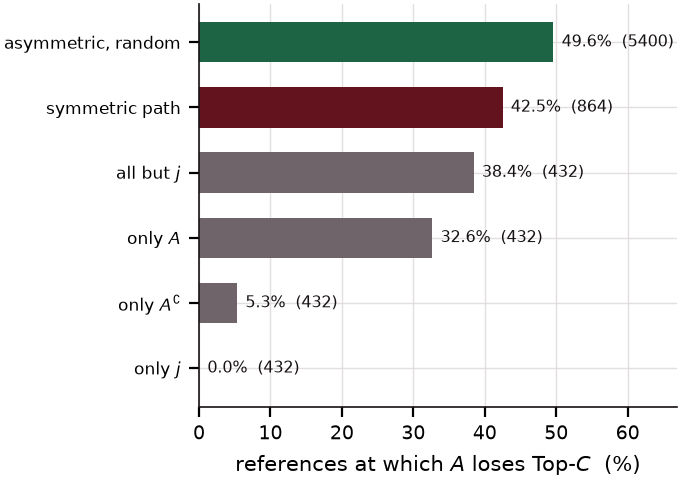
\includegraphics[width=\columnwidth]{d6_fig7_directions.png}
\caption{How often the Top-$C$ set is lost, by the direction the reference is moved in, with
the number of references in each direction in brackets. The symmetric path---the only one the
first sweep used---sits inside the range the other directions span, not at either end:
perturbing only the steered coordinate almost never costs the Top-$C$ property, perturbing
everything but it costs the most among the structured directions, and asymmetric references
drawn independently per coordinate cost more than the symmetric path. Reading the symmetric
path as representative is therefore licensed by measurement rather than by assumption.
\NUM{}}
\label{fig:directions}
\end{figure}

\emph{Sufficiency survives everything tested.} At $\mu=2$, $A$ remains a Top-$C$ set at every
reference in the sweep---$99$ symmetric, $204$ structured and $600$ asymmetric, $903$ in
all---and the doubled regret is non-positive at every one of them.
Theorem~\ref{thm:sufficient} is proved for an arbitrary product reference, so this cannot
confirm it in the logical sense; what it does is exercise the theorem on nine hundred
references outside the corner where the necessity construction lives, including directions
chosen to be awkward, and find no violation. Sufficiency and necessity behave differently off
the corner in exactly the direction the proofs predict. \NUM{}

\begin{figure}[htbp]
\centering
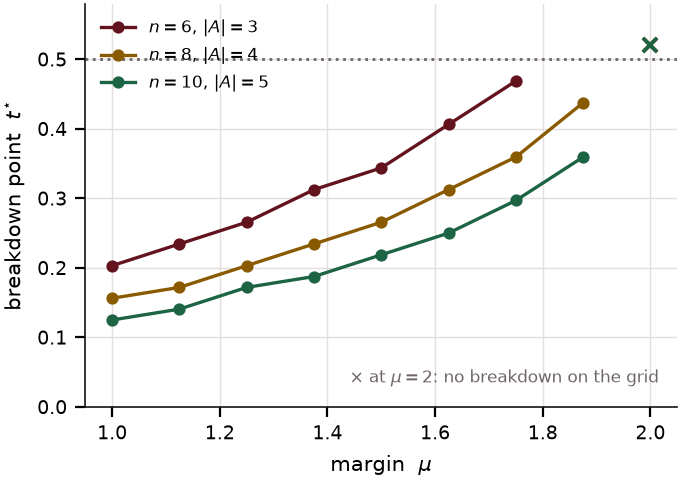
\includegraphics[width=\columnwidth]{d6_fig6_wide.png}
\caption{Where the necessity construction breaks, as a function of the margin, at the three
balanced configurations. Each point is the first $t$ on a sixty-five-point exact grid at
which $A$ stops being a Top-$C$ set, so the hypothesis of
Theorem~\ref{thm:subthreshold} stops holding. The curves rise monotonically with the margin
at every size and fall with the size; the crosses at $\mu=2$ mark that no breakdown occurs
anywhere on the grid there, which is the sufficiency theorem exercised rather than assumed.
Exact rational arithmetic throughout. \NUM{}}
\label{fig:wide}
\end{figure}

\section{Discussion}
\label{sec:discussion}

\subsection{Two Objections of Different Kinds}

The slice objection is about \emph{quantifiers}: it converts a slice-quantified lower bound
into a class-quantified one, and the two-parameter family may now be used without apology.
The provenance objection is about \emph{derivation}: it replaces a fit with an argument, so
the weights are no longer numbers that happened to work in the cells tested. The distinction
matters for how each should be judged, because neither is closed by more data---the $24$ cells
were already consistent, and no quantity of alternatives sampled outside the slice
establishes a universal claim.

Three of the paper's statements sound like limitations and are in fact the contribution.
Corollary~\ref{cor:tight} says the bound cannot be improved by enlarging the class, which
reads as a ceiling but is what makes the reduction free. Theorem~\ref{thm:unique} says there
is no freedom in the weights, which reads as a loss of generality but is what converts a fit
into a derivation. Theorem~\ref{thm:affine} says the optimum is at an endpoint, which reads
as a degenerate answer but is what removes the need to search.

\subsection{Shortcomings and Limitations}
\TODOPAR{Two structural things to settle for the final version. (i) Notation:
$\mu$ denotes both the displacement of the $d$ coordinates in the alternative family
(Sections~I and IV-A) and the margin in the exchange bound (Theorem~\ref{thm:exchange}),
and Theorems~\ref{thm:sufficient}--\ref{thm:subthreshold} then switch to $\rho$ for the same margin while
Section~VII-F switches back. Pick one. (ii) The title carries three propositions and the
margin threshold has nothing to do with the slice or the design; the margin half is a
self-contained result on Top-$C$ selection under approximate modularity and would stand as a
short paper on its own, positioned against Feige--Feldman--Talgam-Cohen on the three axes
Section~II-C already identifies.}

\emph{The reduction is for the scalar query only.} The pair query has a blind direction, so
the coordinate-wise argument of Theorem~\ref{thm:reduction} cannot start: there are non-zero
shifts it cannot see, and no positive lower bound holds uniformly over its class.

\emph{Lower bounds only.} An upper bound quantified over the slice still says nothing about
the class.

\emph{The class is a modelling choice.} An alternative set defined by a norm bound or a
subspace is outside every statement here, and nothing in the formal development can detect a
mismatch, because it is a modelling question. What the development does is make the
hypothesis explicit in the statement.

\emph{The information formulas are premises.} $I_{B}$ and $I_{\mathrm{pair}}$ are taken as
given and not re-derived from the sampling model, so an error in either propagates
downstream---including into \eqref{eq:transitioncond}, which compares them directly.

\emph{The necessity half of the threshold is proved only at the corner.}
Theorem~\ref{thm:subthreshold} is a statement about corner-reference instances and no claim is
proved beyond them. The sweep of Section~\ref{sec:results} shows the situation is better than
that in fact and worse than a theorem: the witness survives a margin-dependent neighbourhood of
the corner and then fails, and $38.1\%$ of the swept positive-$t$ cells lose the Top-$C$
property. Necessity away from the corner is measured, not proved, and this is the most
consequential limitation of the margin results.

\emph{No phase boundary is proved.} Theorem~\ref{thm:affine} identifies where a transition
\emph{can} occur and does not establish that the condition is met anywhere in the parameter
range of interest.

\subsection{Open Problems}

Whether the reduction extends to the pair query, in some form accounting for its blind
direction, is the natural next question. Whether the affine structure survives three or more
query types---where the budget simplex is no longer an interval and an interior optimum
becomes possible---is the second; the objective stays linear so the optimum stays at a
vertex, but the analogue of Proposition~\ref{prop:nonneg} becomes a polytope rather than an
interval and it is not obvious it is cut out as cleanly. Third, whether the sharp threshold
survives a non-corner reference is open: the sweep shows the present construction survives a
margin-dependent neighbourhood of the corner and no further, which locates the question
without settling it.

\section{Conclusion}

The two-parameter alternative family is not a restriction: every alternative in its class
costs at least the slice value, and the bound is attained on the slice. The design
that reproduces the corpus's coefficients is not fitted: it is forced by the budget constraint
and the split, depends only on the split and the price, and makes the delivered information
affine, so the optimal design is pure except on an explicitly computable threshold. And the
margin at which Top-$C$ selection stops being optimal is sharp at $2\delta$: sufficient under
every product reference, and violated below it by an explicit construction under the corner
reference. The wider point concerns how a corpus of results should be maintained. Both
objections answered here were raised against statements that were, numerically, entirely
correct; what was missing in each case was an argument connecting the statement to the claim
it was used to support, and in both cases that argument turned out to be short.

\section*{Acknowledgment}

The formal development uses the Lean~4 theorem prover and the mathlib library.

\begin{thebibliography}{00}

\bibitem{pukelsheim2006} F. Pukelsheim, \emph{Optimal Design of Experiments}. Philadelphia,
PA: SIAM Classics in Applied Mathematics, 2006.

\bibitem{fedorov1972} V. V. Fedorov, \emph{Theory of Optimal Experiments}. New York, NY:
Academic Press, 1972.

\bibitem{boyd2004} S. Boyd and L. Vandenberghe, \emph{Convex Optimization}. Cambridge,
U.K.: Cambridge Univ. Press, 2004.

\bibitem{feige2020} U. Feige, M. Feldman, and I. Talgam-Cohen, ``Approximate modularity
revisited,'' \emph{SIAM J. Comput.}, vol.~49, no.~1, pp.~67--97, 2020.

\bibitem{moore2009} R. E. Moore, R. B. Kearfott, and M. J. Cloud, \emph{Introduction to
Interval Analysis}. Philadelphia, PA: SIAM, 2009.

\bibitem{mathlib2020} The mathlib Community, ``The Lean mathematical library,'' in
\emph{Proc. 9th ACM SIGPLAN Int. Conf. Certified Programs and Proofs (CPP)}, 2020,
pp.~367--381.

\bibitem{demoura2021} L. de Moura and S. Ullrich, ``The Lean 4 theorem prover and
programming language,'' in \emph{Proc. 28th Int. Conf. Automated Deduction (CADE)}, 2021,
pp.~625--635.

\end{thebibliography}

\appendices
\section{Complete statement inventory}
\label{app:inventory}

The D6 strand contributes $187$ axiom-audited theorems and lemmas across its accepted modules. Those that any step of this paper uses are displayed in Section~\ref{sec:setting}, beside the step that consumes them. This appendix reproduces the \emph{complete} chain---every audited statement of the strand, grouped by module, including the ones already shown---so that the development can be read end to end without reassembling it from the body.

Each entry is a symbol-level transliteration of the Lean statement: Unicode maps to the corresponding \LaTeX{} symbol and identifiers are set upright, but no structure is rewritten and no hypothesis is dropped. Binders are listed as the prover has them and the turnstile $\vdash$ separates them from the conclusion. Every entry carries an acceptance receipt and an axiom audit confining it to $\{\textsf{propext},\textsf{Classical.choice},\textsf{Quot.sound}\}$; none contains \texttt{sorry}.

\vspace{4pt}\noindent\rule{\columnwidth}{0.4pt}\par\vspace{2pt}
\noindent\textbf{Module \lean{LeanD6AlternativeReductionV1}}\par\vspace{3pt}

\noindent\textbf{A\,1}\quad\lean{crossing\_bracket}
{\footnotesize\[ \begin{aligned}[t]
&(\mathit{f} : \mathbb{R} \to \mathbb{R} ),\; (\mathit{t0} \mathit{t1} : \mathbb{R} ),\; (\mathit{ht} : \mathit{t0} \leq \mathit{t1}),\; (\mathit{hc} :\\
&\quad \mathit{ContinuousOn} \mathit{f} (\mathit{Set}.\mathit{Icc} \mathit{t0} \mathit{t1})),\; (\mathit{h0} : \mathit{f} \mathit{t0} \leq 0),\; (\mathit{h1} : 0 \leq \mathit{f} \mathit{t1})\\
\vdash\;&\exists \mathit{t} \in \mathit{Set}.\mathit{Icc} \mathit{t0} \mathit{t1}, \mathit{f} \mathit{t} = 0
\end{aligned} \]}

\noindent\textbf{A\,2}\quad\lean{no\_crossing\_of\_modulus}
{\footnotesize\[ \begin{aligned}[t]
&(\mathit{f} : \mathbb{R} \to \mathbb{R} ),\; (\mathit{t0} \mathit{t1} \mathit{Lip} \mathit{m} : \mathbb{R} ),\; (\mathit{ht} : \mathit{t0} \leq \mathit{t1}),\\
&\quad \; (\mathit{hLip} : 0 \leq \mathit{Lip}),\; (\mathit{hlip} : \forall \mathit{s} \in \mathit{Set}.\mathit{Icc} \mathit{t0} \mathit{t1}, |\mathit{f} \mathit{s} - \mathit{f} \mathit{t0}| \leq\\
&\quad \mathit{Lip} * (\mathit{s} - \mathit{t0})),\; (\mathit{hm} : \mathit{m} \leq \mathit{f} \mathit{t0}),\; (\mathit{hpos} : 0 < \mathit{m}),\\
&\quad \; (\mathit{hgap} : \mathit{Lip} * (\mathit{t1} - \mathit{t0}) < \mathit{m})\\
\vdash\;&\forall \mathit{t} \in \mathit{Set}.\mathit{Icc} \mathit{t0} \mathit{t1}, 0 < \mathit{f} \mathit{t}
\end{aligned} \]}

\noindent\textbf{A\,3}\quad\lean{quadratic\_ge\_vertex}
{\footnotesize\[ \begin{aligned}[t]
&(\mathit{a} \mathit{b} \mathit{c} \mathit{x} : \mathbb{R} ),\; (\mathit{ha} : 0 < \mathit{a})\\
\vdash\;&\mathit{a} * (-\mathit{b} / (2 * \mathit{a})) ^{2} + \mathit{b} * (-\mathit{b} / (2 * \mathit{a})) + \mathit{c} \leq\\
&\quad \mathit{a} * \mathit{x} ^{2} + \mathit{b} * \mathit{x} + \mathit{c}
\end{aligned} \]}

\noindent\textbf{A\,4}\quad\lean{quadratic\_inf\_Icc}
{\footnotesize\[ \begin{aligned}[t]
&(\mathit{a} \mathit{b} \mathit{c} \mathit{lo} \mathit{hi} \mathit{x} : \mathbb{R} ),\; (\mathit{ha} : 0 < \mathit{a}),\; (\mathit{hx1} : \mathit{lo} \leq \mathit{x}),\; (\mathit{hx2} : \mathit{x} \leq \mathit{hi})\\
\vdash\;&\mathit{min} (\mathit{min} (\mathit{a} * \mathit{lo} ^{2} + \mathit{b} * \mathit{lo} + \mathit{c}) (\mathit{a} * \mathit{hi} ^{2} + \mathit{b} * \mathit{hi} + \mathit{c})) (\mathit{a} * (-\\
&\quad \mathit{b} / (2 * \mathit{a})) ^{2} + \mathit{b} * (-\mathit{b} / (2 * \mathit{a})) + \mathit{c}) \leq \mathit{a} * \mathit{x} ^{2} + \mathit{b} * \mathit{x} + \mathit{c}
\end{aligned} \]}

\noindent\textbf{A\,5}\quad\lean{quadratic\_inf\_attained}
{\footnotesize\[ \begin{aligned}[t]
&(\mathit{a} \mathit{b} \mathit{c} \mathit{lo} \mathit{hi} : \mathbb{R} ),\; (\mathit{ha} : 0 < \mathit{a}),\; (\mathit{hv1} : \mathit{lo} \leq -\mathit{b} / (2 * \mathit{a})),\\
&\quad \; (\mathit{hv2} : -\mathit{b} / (2 * \mathit{a}) \leq \mathit{hi})\\
\vdash\;&(\forall \mathit{x}, \mathit{lo} \leq \mathit{x} \to \mathit{x} \leq \mathit{hi} \to \mathit{a} * (-\mathit{b} / (2 * \mathit{a})) ^{2} + \mathit{b} * (-\mathit{b} / (\\
&\quad 2 * \mathit{a})) + \mathit{c} \leq \mathit{a} * \mathit{x} ^{2} + \mathit{b} * \mathit{x} + \mathit{c}) \wedge \mathit{lo} \leq -\mathit{b} / (2 * \mathit{a}) \wedge\\
&\quad -\mathit{b} / (2 * \mathit{a}) \leq \mathit{hi}
\end{aligned} \]}

\noindent\textbf{A\,6}\quad\lean{quadratic\_inf\_endpoint\_left}
{\footnotesize\[ \begin{aligned}[t]
&(\mathit{a} \mathit{b} \mathit{c} \mathit{lo} \mathit{hi} \mathit{x} : \mathbb{R} ),\; (\mathit{ha} : 0 < \mathit{a}),\; (\mathit{hv} : -\mathit{b} / (2 * \mathit{a}) \leq \mathit{lo}),\\
&\quad \; (\mathit{hx1} : \mathit{lo} \leq \mathit{x}),\; (\mathit{hx2} : \mathit{x} \leq \mathit{hi})\\
\vdash\;&\mathit{a} * \mathit{lo} ^{2} + \mathit{b} * \mathit{lo} + \mathit{c} \leq \mathit{a} * \mathit{x} ^{2} + \mathit{b} * \mathit{x} + \mathit{c}
\end{aligned} \]}

\noindent\textbf{A\,7}\quad\lean{quadratic\_inf\_endpoint\_right}
{\footnotesize\[ \begin{aligned}[t]
&(\mathit{a} \mathit{b} \mathit{c} \mathit{lo} \mathit{hi} \mathit{x} : \mathbb{R} ),\; (\mathit{ha} : 0 < \mathit{a}),\; (\mathit{hv} : \mathit{hi} \leq -\mathit{b} / (2 * \mathit{a})),\\
&\quad \; (\mathit{hx1} : \mathit{lo} \leq \mathit{x}),\; (\mathit{hx2} : \mathit{x} \leq \mathit{hi})\\
\vdash\;&\mathit{a} * \mathit{hi} ^{2} + \mathit{b} * \mathit{hi} + \mathit{c} \leq \mathit{a} * \mathit{x} ^{2} + \mathit{b} * \mathit{x} + \mathit{c}
\end{aligned} \]}

\vspace{4pt}\noindent\rule{\columnwidth}{0.4pt}\par\vspace{2pt}
\noindent\textbf{Module \lean{LeanD6ApproximateActualEvaluatorV1}}\par\vspace{3pt}

\noindent\textbf{A\,8}\quad\lean{actual\_label\_infimum}
{\footnotesize\[ \begin{aligned}[t]
&(\mathit{A} \mathit{B} \mathit{C} : \mathit{Finset} (\mathit{I} \mathit{n})),\; (\mathit{j} : \mathit{I} \mathit{n}),\; (\mathit{hjC} : \mathit{j} \notin \mathit{C}),\; (\mathit{q} \mathit{mu} \mathit{eps} : \mathbb{R} ),\\
&\quad \; (\mathit{he} : 0 \leq \mathit{eps}),\; (\mathit{hd} : \mathit{eps} < (\mathit{exchange} \mathit{C} \mathit{B} : \mathbb{R} )),\\
&\quad \; (\mathit{E} : \mathit{Finset} (\mathit{Measurement} \mathit{n})),\; (\mathit{w} : \mathit{Measurement} \mathit{n} \to \mathbb{R} ),\\
&\quad \; (\mathit{hl} : \forall \mathit{e} \in \mathit{E},\mathit{Legal} \mathit{j} \mathit{q} \mathit{e}),\; (\mathit{hw} : \forall \mathit{e} \in \mathit{E},0 \leq \mathit{w} \mathit{e})\\
\vdash\;&\mathit{sInf} (\mathit{labelCosts} \mathit{A} \mathit{B} \mathit{C} \mathit{j} \mathit{mu} \mathit{eps} \mathit{E} \mathit{w})=\mathit{evaluator} \mathit{A} \mathit{B} \mathit{C} \mathit{j} \mathit{mu} \mathit{eps} \mathit{E} \mathit{w}
\end{aligned} \]}

\noindent\textbf{A\,9}\quad\lean{curvature\_nonneg}
{\footnotesize\[ \begin{aligned}[t]
&(\mathit{B} : \mathit{Finset} (\mathit{I} \mathit{n})),\; (\mathit{j} : \mathit{I} \mathit{n}),\; (\mathit{E} : \mathit{Finset} (\mathit{Measurement} \mathit{n})),\\
&\quad \; (\mathit{w} : \mathit{Measurement} \mathit{n} \to \mathbb{R} ),\; (\mathit{hw} : \forall \mathit{e} \in \mathit{E},0 \leq \mathit{w} \mathit{e})\\
\vdash\;&0 \leq \mathit{curvature} \mathit{B} \mathit{j} \mathit{E} \mathit{w}
\end{aligned} \]}

\noindent\textbf{A\,10}\quad\lean{zero\_curvature\_cross}
{\footnotesize\[ \begin{aligned}[t]
&(\mathit{A} \mathit{B} : \mathit{Finset} (\mathit{I} \mathit{n})),\; (\mathit{j} : \mathit{I} \mathit{n}),\; (\mathit{mu} : \mathbb{R} ),\; (\mathit{E} : \mathit{Finset} (\\
&\quad \mathit{Measurement} \mathit{n})),\; (\mathit{w} : \mathit{Measurement} \mathit{n} \to \mathbb{R} ),\; (\mathit{hw} : \forall \mathit{e} \in \mathit{E},\\
&\quad 0 \leq \mathit{w} \mathit{e}),\; (\mathit{hc} : \mathit{curvature} \mathit{B} \mathit{j} \mathit{E} \mathit{w}=0)\\
\vdash\;&\mathit{crossTerm} \mathit{A} \mathit{B} \mathit{j} \mathit{mu} \mathit{E} \mathit{w}=0
\end{aligned} \]}

\vspace{4pt}\noindent\rule{\columnwidth}{0.4pt}\par\vspace{2pt}
\noindent\textbf{Module \lean{LeanD6CalibrationActiveFaceV1}}\par\vspace{3pt}

\noindent\textbf{A\,11}\quad\lean{active\_iff\_cross\_zero}
{\footnotesize\[ \begin{aligned}[t]
&(\mathit{D} \mathit{M} : \mathit{Alt} \to \mathbb{R} ),\; (\mathit{Gamma} : \mathbb{R} ),\; (\mathit{a} : \mathit{Alt}),\; (\mathit{hactive} : \mathit{D} \mathit{a} =\\
&\quad \mathit{Gamma})\\
\vdash\;&\mathit{Gamma} \leq \mathit{profiled} \mathit{D} \mathit{M} \mathit{a} \leftrightarrow \mathit{M} \mathit{a} = 0
\end{aligned} \]}

\noindent\textbf{A\,12}\quad\lean{active\_nonzero\_forces\_loss}
{\footnotesize\[ \begin{aligned}[t]
&(\mathit{D} \mathit{M} : \mathit{Alt} \to \mathbb{R} ),\; (\mathit{Gamma} : \mathbb{R} ),\; (\mathit{a} : \mathit{Alt}),\; (\mathit{hactive} : \mathit{D} \mathit{a} =\\
&\quad \mathit{Gamma}),\; (\mathit{hcross} : \mathit{M} \mathit{a} \neq 0)\\
\vdash\;&\mathit{profiled} \mathit{D} \mathit{M} \mathit{a} < \mathit{Gamma}
\end{aligned} \]}

\noindent\textbf{A\,13}\quad\lean{profile\_formula\_unit}
{\footnotesize\[ \begin{aligned}[t]
&\{ \mathit{E} : \mathit{Type}*\},\; [\mathit{Fintype} \mathit{E}],\; (\mathit{w} \mathit{d} : \mathit{E} \to \mathbb{R} ),\; (\mathit{hcurv} : \mathit{curvature} \mathit{w} (\\
&\quad \mathbf{fun} \mathit{\_} => 1) = 1)\\
\vdash\;&\mathit{energy} \mathit{w} \mathit{d} (\mathbf{fun} \mathit{\_} => 1) (\mathit{cross} \mathit{w} \mathit{d} (\mathbf{fun} \mathit{\_} => 1)) =\\
&\quad \mathit{raw} \mathit{w} \mathit{d} / 2 - (\mathit{cross} \mathit{w} \mathit{d} (\mathbf{fun} \mathit{\_} => 1))^{2} / 2
\end{aligned} \]}

\noindent\textbf{A\,14}\quad\lean{profiled\_ge\_iff}
{\footnotesize\[ \begin{aligned}[t]
&(\mathit{D} \mathit{M} : \mathit{Alt} \to \mathbb{R} ),\; (\mathit{Gamma} : \mathbb{R} ),\; (\mathit{hknown} : \forall \mathit{a}, \mathit{Gamma} \leq \mathit{D} \mathit{a})\\
\vdash\;&(\forall \mathit{a}, \mathit{Gamma} \leq \mathit{profiled} \mathit{D} \mathit{M} \mathit{a}) \leftrightarrow \forall \mathit{a}, (\mathit{M} \mathit{a})^{2} \leq 2 * \mathit{slack} \mathit{D} \mathit{Gamma}\\
&\quad \mathit{a}
\end{aligned} \]}

\vspace{4pt}\noindent\rule{\columnwidth}{0.4pt}\par\vspace{2pt}
\noindent\textbf{Module \lean{LeanD6CenterAnswerGeometryV1}}\par\vspace{3pt}

\noindent\textbf{A\,15}\quad\lean{boundary\_arbitrarily\_small}
{\footnotesize\[ \begin{aligned}[t]
&(\mathit{A} \mathit{B} : \mathit{Finset} (\mathit{I} \mathit{n})),\; (\mathit{j} : \mathit{I} \mathit{n}),\; (\mathit{hj} : \mathit{j} \notin \mathit{A}),\; (\mathit{q} \mathit{mu} : \mathbb{R} ),\\
&\quad \; (\mathit{hmu0} : 0 < \mathit{mu}),\; (\mathit{hmu1} : \mathit{mu} \leq 1),\; (\mathit{E} : \mathit{Finset} (\\
&\quad \mathit{Measurement} \mathit{n})),\; (\mathit{w} : \mathit{Measurement} \mathit{n} \to \mathbb{R} ),\; (\mathit{hl} : \forall \mathit{e} \in \mathit{E},\\
&\quad \mathit{Legal} \mathit{j} \mathit{q} \mathit{e}),\; (\mathit{hw} : \forall \mathit{e} \in \mathit{E}, 0 \leq \mathit{w} \mathit{e}),\; (\mathit{hd} : 0 <\\
&\quad \mathit{exchange} \mathit{A} \mathit{B}),\; (\mathit{target} : \mathbb{R} ),\; (\mathit{htarget} : 0 < \mathit{target})\\
\vdash\;&\exists \mathit{eta} : \mathbb{R} , 0 < \mathit{eta} \wedge \mathit{eta} \leq \mathit{mu} \wedge \mathit{BadNuisance} (\mathit{exchange} \mathit{A}\\
&\quad \mathit{B}) ((2-\mathit{mu})*(\mathit{exchange} \mathit{A} \mathit{B}:\mathbb{R} )/2) (\mathit{mu}-\mathit{eta}) \wedge\\
&\quad (\textstyle\sum \mathit{e} \in \mathit{E},\mathit{w} \mathit{e}*\mathit{information} \mathit{A} \mathit{A} \mathit{j} \mathit{mu} (\mathit{mu}-\mathit{eta}) \mathit{e}) < \mathit{target}
\end{aligned} \]}

\noindent\textbf{A\,16}\quad\lean{boundary\_same\_label\_bad}
{\footnotesize\[ \begin{aligned}[t]
&(\mathit{d} : \mathbb{N} ),\; (\mathit{hd} : 0 < \mathit{d}),\; (\mathit{mu} \mathit{eta} : \mathbb{R} ),\; (\mathit{hmu} : \mathit{mu} \leq 1),\\
&\quad \; (\mathit{heta} : 0 < \mathit{eta}),\; (\mathit{hle} : \mathit{eta} \leq \mathit{mu})\\
\vdash\;&\mathit{BadNuisance} \mathit{d} ((2-\mathit{mu})*(\mathit{d}:\mathbb{R} )/2) (\mathit{mu}-\mathit{eta})
\end{aligned} \]}

\noindent\textbf{A\,17}\quad\lean{same\_label\_path\_information}
{\footnotesize\[ \begin{aligned}[t]
&(\mathit{A} : \mathit{Finset} (\mathit{I} \mathit{n})),\; (\mathit{j} : \mathit{I} \mathit{n}),\; (\mathit{hj} : \mathit{j} \notin \mathit{A}),\; (\mathit{q} \mathit{mu} \mathit{eta} : \mathbb{R} ),\\
&\quad \; (\mathit{e} : \mathit{Measurement} \mathit{n}),\; (\mathit{he} : \mathit{Legal} \mathit{j} \mathit{q} \mathit{e})\\
\vdash\;&\mathit{information} \mathit{A} \mathit{A} \mathit{j} \mathit{mu} (\mathit{mu}-\mathit{eta}) \mathit{e} = (\mathit{meanSlope} \mathit{A} \mathit{j} \mathit{e})^{2}*\mathit{eta}^{2}/2
\end{aligned} \]}

\noindent\textbf{A\,18}\quad\lean{same\_label\_path\_sum}
{\footnotesize\[ \begin{aligned}[t]
&(\mathit{A} : \mathit{Finset} (\mathit{I} \mathit{n})),\; (\mathit{j} : \mathit{I} \mathit{n}),\; (\mathit{hj} : \mathit{j} \notin \mathit{A}),\; (\mathit{q} \mathit{mu} \mathit{eta} : \mathbb{R} ),\\
&\quad \; (\mathit{E} : \mathit{Finset} (\mathit{Measurement} \mathit{n})),\; (\mathit{w} : \mathit{Measurement} \mathit{n} \to \mathbb{R} ),\\
&\quad \; (\mathit{hl} : \forall \mathit{e} \in \mathit{E}, \mathit{Legal} \mathit{j} \mathit{q} \mathit{e})\\
\vdash\;&(\textstyle\sum \mathit{e} \in \mathit{E}, \mathit{w} \mathit{e} * \mathit{information} \mathit{A} \mathit{A} \mathit{j} \mathit{mu} (\mathit{mu}-\mathit{eta}) \mathit{e}) =\\
&\quad \mathit{eta}^{2}/2 * \mathit{curvature} \mathit{A} \mathit{j} \mathit{E} \mathit{w}
\end{aligned} \]}

\vspace{4pt}\noindent\rule{\columnwidth}{0.4pt}\par\vspace{2pt}
\noindent\textbf{Module \lean{LeanD6CyclicValueConfidenceV1}}\par\vspace{3pt}

\noindent\textbf{A\,19}\quad\lean{actual\_world\_value\_confidence}
{\footnotesize\[ \begin{aligned}[t]
&(\mathit{q} : \mathbb{N} ),\; (\mathit{hq} : 3 \leq \mathit{q}),\; (\mathit{j} : \mathit{I} (2*\mathit{q}+1))\\
\vdash\;&\exists \mathit{G} : \mathit{ZMod} (2*\mathit{q}+1) \to \mathit{Finset} (\mathit{I} (2*\mathit{q}+1)),\\
&\quad (\forall \mathit{t},\mathit{Legal} \mathit{j} \mathit{q} (.\mathit{inr} (\mathit{G} \mathit{t},\mathit{false})) \wedge (\mathit{G} \mathit{t}).\mathit{card}=\mathit{q}) \wedge\\
&\quad \forall \mathit{A} : \mathit{Finset} (\mathit{I} (2*\mathit{q}+1)), \mathit{A} \in \mathit{worlds} \mathit{q} \mathit{j} \to \forall \mathit{L0} : \mathbb{N} ,0 <\\
&\quad \mathit{L0} \to \forall \mathit{mu} \mathit{delta} : \mathbb{R} ,0 \leq \mathit{mu} \to \mathit{mu} \leq 1 \to 0 < \mathit{delta} \to\\
&\quad \mathit{delta} \leq 1 \to \forall (\mathit{E} : \mathit{Finset} (\mathit{Measurement} (2*\mathit{q}+1))) (\mathit{w} \mathit{v} : \mathbb{N}\\
&\quad \to \mathit{Sample} (\mathit{ZMod} (2*\mathit{q}+1)) \to \mathit{Measurement} (2*\mathit{q}+1) \to\\
&\quad \mathbb{R} ) (\mathit{tau} : \mathbb{N} \to \mathit{Sample} (\mathit{ZMod} (2*\mathit{q}+1)) \to \mathbb{R} ), (\forall \mathit{s} \mathit{x},0 \leq\\
&\quad \mathit{tau} \mathit{s} \mathit{x}) \to (\forall \mathit{s} \mathit{x},\mathit{Feasible} \mathit{j} \mathit{q} \mathit{E} (\mathit{w} \mathit{s} \mathit{x})) \to (\forall \mathit{s} \mathit{x} \mathit{e},\mathit{e} \in \mathit{E} \to 0 \leq\\
&\quad \mathit{v} \mathit{s} \mathit{x} \mathit{e}) \to (\forall \mathit{s} \mathit{x},\mathit{oracleValue} \mathit{A} \mathit{j} \mathit{q} (\mathit{modelEstimate} \mathit{q} \mathit{L0} \mathit{s} \mathit{x}) \leq\\
&\quad \mathit{allocationValue} \mathit{A} \mathit{j} (\mathit{modelEstimate} \mathit{q} \mathit{L0} \mathit{s} \mathit{x}) \mathit{E} (\mathit{w} \mathit{s} \mathit{x})+\mathit{tau} \mathit{s} \mathit{x})\\
&\quad \to (\mathit{path} \mathit{G} \mathit{A} \mathit{j} \mathit{mu}) (⋃ \mathit{s} : \mathbb{N} ,\{ \mathit{x} | 2*\mathit{marginModulus} \mathit{q}*\mathit{width} (\mathit{C}
\end{aligned} \]}

\noindent\textbf{A\,20}\quad\lean{cyclic\_value\_confidence}
{\footnotesize\[ \begin{aligned}[t]
&(\mathit{G} : \mathit{C} \to \mathit{Finset} (\mathit{I} \mathit{n})),\; (\mathit{A} : \mathit{Finset} (\mathit{I} \mathit{n})),\; (\mathit{j} : \mathit{I} \mathit{n}),\\
&\quad \; (\mathit{hj} : \mathit{j} \notin \mathit{A}),\; (\mathit{halt} : \exists \mathit{A'} \mathit{nu},\mathit{Admissible} \mathit{A} \mathit{A'} \mathit{j} \mathit{nu}),\; (\mathit{q} \mathit{L0} : \mathbb{N} ),\\
&\quad \; (\mathit{hq} : 1 \leq \mathit{q}),\; (\mathit{hL} : 0 < \mathit{L0}),\; (\mathit{hC} : 0 < \mathit{Fintype}.\mathit{card} \mathit{C}),\\
&\quad \; (\mathit{mu} : \mathbb{R} ),\; (\mathit{hmu} : 0 \leq \mathit{mu}),\; (\mathit{hmu1} : \mathit{mu} \leq 1),\; (\mathit{hm} : (\textstyle\sum \mathit{t},\\
&\quad \mathit{actualMean} \mathit{A} \mathit{j} \mathit{mu} (.\mathit{inr} (\mathit{G} \mathit{t},\mathit{false}))) = \mathit{Fintype}.\mathit{card} \mathit{C}+(\mathit{q}:\mathbb{R}\\
&\quad )^{2}*(1-\mathit{mu})),\; (\mathit{delta} : \mathbb{R} ),\; (\mathit{hd} : 0 < \mathit{delta}),\\
&\quad \; (\mathit{hd1} : \mathit{delta} \leq 1),\; (\mathit{E} : \mathit{Finset} (\mathit{Measurement} \mathit{n})),\\
&\quad \; (\mathit{w} \mathit{v} : \mathbb{N} \to \mathit{Sample} \mathit{C} \to \mathit{Measurement} \mathit{n} \to \mathbb{R} ),\; (\mathit{tau} : \mathbb{N} \to\\
&\quad \mathit{Sample} \mathit{C} \to \mathbb{R} ),\; (\mathit{ht} : \forall \mathit{s} \mathit{x},0 \leq \mathit{tau} \mathit{s} \mathit{x}),\; (\mathit{hf} : \forall \mathit{s} \mathit{x},\\
&\quad \mathit{Feasible} \mathit{j} \mathit{q} \mathit{E} (\mathit{w} \mathit{s} \mathit{x})),\; (\mathit{hv} : \forall \mathit{s} \mathit{x} \mathit{e},\mathit{e} \in \mathit{E} \to 0 \leq \mathit{v} \mathit{s} \mathit{x} \mathit{e}),\\
&\quad \; (\mathit{hopt} : \forall \mathit{s} \mathit{x},\mathit{oracleValue} \mathit{A} \mathit{j} \mathit{q} (\mathit{modelEstimate} \mathit{q} \mathit{L0} \mathit{s} \mathit{x}) \leq\\
&\quad \mathit{allocationValue} \mathit{A} \mathit{j} (\mathit{modelEstimate} \mathit{q} \mathit{L0} \mathit{s} \mathit{x}) \mathit{E} (\mathit{w} \mathit{s} \mathit{x})+\mathit{tau} \mathit{s} \mathit{x})\\
\vdash\;&(\mathit{path} \mathit{G} \mathit{A} \mathit{j} \mathit{mu}) (⋃ \mathit{s} : \mathbb{N} ,\{ \mathit{x} | 2*\mathit{marginModulus} \mathit{q}*\mathit{width} (\mathit{C}
\end{aligned} \]}

\noindent\textbf{A\,21}\quad\lean{model\_estimate\_mem}
{\footnotesize\[ \begin{aligned}[t]
&(\mathit{q} \mathit{L0} \mathit{s} : \mathbb{N} ),\; (\mathit{x} : \mathit{Sample} \mathit{C})\\
\vdash\;&0 \leq \mathit{modelEstimate} \mathit{q} \mathit{L0} \mathit{s} \mathit{x} \wedge \mathit{modelEstimate} \mathit{q} \mathit{L0} \mathit{s} \mathit{x} \leq 1
\end{aligned} \]}

\vspace{4pt}\noindent\rule{\columnwidth}{0.4pt}\par\vspace{2pt}
\noindent\textbf{Module \lean{LeanD6DesignDerivationV1}}\par\vspace{3pt}

\noindent\textbf{A\,22}\quad\lean{budget\_exact}
{\footnotesize\[ (\mathit{eta} \mathit{c} : \mathbb{Q} ),\; (\mathit{hc} : \mathit{c} \neq 0) \;\vdash\; \mathit{wB} \mathit{eta} + \mathit{c} * \mathit{wPair} \mathit{eta} \mathit{c} = 1 \]}

\noindent\textbf{A\,23}\quad\lean{flat\_when\_equal\_price}
{\footnotesize\[ \begin{aligned}[t]
&(\mathit{IB} \mathit{Ipair} \mathit{c} : \mathbb{Q} ),\; (\mathit{hc} : \mathit{c} \neq 0),\; (\mathit{heq} : \mathit{Ipair} / \mathit{c} - \mathit{IB} = 0),\\
&\quad \; (\mathit{eta} \mathit{eta'} : \mathbb{Q} )\\
\vdash\;&\mathit{info} \mathit{IB} \mathit{Ipair} \mathit{eta} \mathit{c} = \mathit{info} \mathit{IB} \mathit{Ipair} \mathit{eta'} \mathit{c}
\end{aligned} \]}

\noindent\textbf{A\,24}\quad\lean{info\_linear}
{\footnotesize\[ \begin{aligned}[t]
&(\mathit{IB} \mathit{Ipair} \mathit{eta} \mathit{c} : \mathbb{Q} ),\; (\mathit{hc} : \mathit{c} \neq 0)\\
\vdash\;&\mathit{info} \mathit{IB} \mathit{Ipair} \mathit{eta} \mathit{c} = \mathit{IB} + \mathit{eta} * (\mathit{Ipair} / \mathit{c} - \mathit{IB})
\end{aligned} \]}

\noindent\textbf{A\,25}\quad\lean{optimum\_at\_endpoint}
{\footnotesize\[ \begin{aligned}[t]
&(\mathit{IB} \mathit{Ipair} \mathit{c} : \mathbb{Q} ),\; (\mathit{hc} : \mathit{c} \neq 0),\; (\mathit{eta} : \mathbb{Q} ),\; (\mathit{h0} : 0 \leq \mathit{eta}),\\
&\quad \; (\mathit{h1} : \mathit{eta} \leq 1)\\
\vdash\;&\mathit{info} \mathit{IB} \mathit{Ipair} \mathit{eta} \mathit{c} \leq \mathit{max} (\mathit{info} \mathit{IB} \mathit{Ipair} 0 \mathit{c}) (\mathit{info} \mathit{IB} \mathit{Ipair} 1 \mathit{c})
\end{aligned} \]}

\noindent\textbf{A\,26}\quad\lean{transition\_at\_equal\_price}
{\footnotesize\[ \begin{aligned}[t]
&(\mathit{IB} \mathit{Ipair} \mathit{c} : \mathbb{Q} ),\; (\mathit{hc} : 0 < \mathit{c})\\
\vdash\;&(\mathit{Ipair} / \mathit{c} - \mathit{IB} = 0) \leftrightarrow \mathit{c} * \mathit{IB} = \mathit{Ipair}
\end{aligned} \]}

\noindent\textbf{A\,27}\quad\lean{weights\_nonneg\_iff}
{\footnotesize\[ \begin{aligned}[t]
&(\mathit{eta} \mathit{c} : \mathbb{Q} ),\; (\mathit{hc} : 0 < \mathit{c})\\
\vdash\;&(0 \leq \mathit{wB} \mathit{eta} \wedge 0 \leq \mathit{wPair} \mathit{eta} \mathit{c}) \leftrightarrow (0 \leq \mathit{eta} \wedge \mathit{eta} \leq 1)
\end{aligned} \]}

\noindent\textbf{A\,28}\quad\lean{weights\_unique}
{\footnotesize\[ \begin{aligned}[t]
&(\mathit{eta} \mathit{c} \mathit{a} \mathit{b} : \mathbb{Q} ),\; (\mathit{hc} : \mathit{c} \neq 0),\; (\mathit{hbudget} : \mathit{a} + \mathit{c} * \mathit{b} = 1),\\
&\quad \; (\mathit{hshare} : \mathit{c} * \mathit{b} = \mathit{eta})\\
\vdash\;&\mathit{a} = \mathit{wB} \mathit{eta} \wedge \mathit{b} = \mathit{wPair} \mathit{eta} \mathit{c}
\end{aligned} \]}

\vspace{4pt}\noindent\rule{\columnwidth}{0.4pt}\par\vspace{2pt}
\noindent\textbf{Module \lean{LeanD6GeneralFamilyV1}}\par\vspace{3pt}

\noindent\textbf{A\,29}\quad\lean{IB\_eq\_of\_slice}
{\footnotesize\[ \begin{aligned}[t]
&(\mathit{q} : \mathbb{N} ),\; (\mathit{hq} : 0 < \mathit{q}),\; (\mathit{mu} \mathit{x} : \mathbb{Q} ),\; (\mathit{v} : \mathit{Fin} \mathit{q} \to \mathbb{Q} ),\\
&\quad \; (\mathit{S} : \mathit{Finset} (\mathit{Fin} \mathit{q})),\; (\mathit{hS} : \forall \mathit{i} \in \mathit{S}, \mathit{v} \mathit{i} = \mathit{mu}),\\
&\quad \; (\mathit{hSc} : \forall \mathit{i}, \mathit{i} \notin \mathit{S} \to \mathit{v} \mathit{i} = \mathit{x})\\
\vdash\;&\mathit{Igen} \mathit{q} \mathit{v} = \mathit{IB} (\mathit{q} : \mathbb{Q} ) (\mathit{S}.\mathit{card} : \mathbb{Q} ) \mathit{mu} \mathit{x}
\end{aligned} \]}

\noindent\textbf{A\,30}\quad\lean{IB\_le\_general}
{\footnotesize\[ \begin{aligned}[t]
&(\mathit{q} : \mathbb{N} ),\; (\mathit{hq} : 0 < \mathit{q}),\; (\mathit{mu} \mathit{x} : \mathbb{Q} ),\; (\mathit{hmu} : 0 \leq \mathit{mu}),\\
&\quad \; (\mathit{hx} : 0 \leq \mathit{x}),\; (\mathit{v} : \mathit{Fin} \mathit{q} \to \mathbb{Q} ),\; (\mathit{S} : \mathit{Finset} (\mathit{Fin} \mathit{q})),\\
&\quad \; (\mathit{hS} : \forall \mathit{i} \in \mathit{S}, \mathit{mu} \leq |\mathit{v} \mathit{i}|),\; (\mathit{hSc} : \forall \mathit{i}, \mathit{i} \notin \mathit{S} \to \mathit{x} \leq |\mathit{v} \mathit{i}|)\\
\vdash\;&\mathit{IB} (\mathit{q} : \mathbb{Q} ) (\mathit{S}.\mathit{card} : \mathbb{Q} ) \mathit{mu} \mathit{x} \leq \mathit{Igen} \mathit{q} \mathit{v}
\end{aligned} \]}

\noindent\textbf{A\,31}\quad\lean{Igen\_nonneg}
{\footnotesize\[ (\mathit{q} : \mathbb{N} ),\; (\mathit{v} : \mathit{Fin} \mathit{q} \to \mathbb{Q} ) \;\vdash\; 0 \leq \mathit{Igen} \mathit{q} \mathit{v} \]}

\noindent\textbf{A\,32}\quad\lean{Igen\_pos\_of\_ne\_zero}
{\footnotesize\[ \begin{aligned}[t]
&(\mathit{q} : \mathbb{N} ),\; (\mathit{hq} : 0 < \mathit{q}),\; (\mathit{v} : \mathit{Fin} \mathit{q} \to \mathbb{Q} ),\; (\mathit{i₀} : \mathit{Fin} \mathit{q}),\\
&\quad \; (\mathit{hne} : \mathit{v} \mathit{i₀} \neq 0)\\
\vdash\;&0 < \mathit{Igen} \mathit{q} \mathit{v}
\end{aligned} \]}

\noindent\textbf{A\,33}\quad\lean{slice\_is\_tight}
{\footnotesize\[ \begin{aligned}[t]
&(\mathit{q} : \mathbb{N} ),\; (\mathit{hq} : 0 < \mathit{q}),\; (\mathit{mu} \mathit{x} : \mathbb{Q} ),\; (\mathit{v} : \mathit{Fin} \mathit{q} \to \mathbb{Q} ),\\
&\quad \; (\mathit{S} : \mathit{Finset} (\mathit{Fin} \mathit{q})),\; (\mathit{hS} : \forall \mathit{i} \in \mathit{S}, \mathit{v} \mathit{i} = \mathit{mu}),\\
&\quad \; (\mathit{hSc} : \forall \mathit{i}, \mathit{i} \notin \mathit{S} \to \mathit{v} \mathit{i} = \mathit{x})\\
\vdash\;&\mathit{Igen} \mathit{q} \mathit{v} = \mathit{IB} (\mathit{q} : \mathbb{Q} ) (\mathit{S}.\mathit{card} : \mathbb{Q} ) \mathit{mu} \mathit{x}
\end{aligned} \]}

\vspace{4pt}\noindent\rule{\columnwidth}{0.4pt}\par\vspace{2pt}
\noindent\textbf{Module \lean{LeanD6MarginSensitiveExchangeV1}}\par\vspace{3pt}

\noindent\textbf{A\,34}\quad\lean{pair\_doubled\_loss\_le\_card\_mul\_two\_delta\_sub\_margin}
{\footnotesize\[ \begin{aligned}[t]
&\{ \mathit{n} : \mathbb{N} \},\; (\mathit{q} : \mathit{Fin} (\mathit{n} + 1) \to \mathit{U} \to \mathbb{R} ),\; (\mathit{F} : (\mathit{Fin} (\mathit{n} + 1) \to \mathit{U})\\
&\quad \to \mathbb{R} ),\; (\mathit{delta} \mathit{mu} : \mathbb{R} ),\; (\mathit{hWeight} : \forall \mathit{c}, 0 \leq\\
&\quad \mathit{jointWeight} \mathit{q} \mathit{c}),\; (\mathit{hNorm} : \textstyle\sum \mathit{c}, \mathit{jointWeight} \mathit{q} \mathit{c} = 1),\\
&\quad \; (\mathit{hDeltaNonneg} : 0 \leq \mathit{delta}),\; (\mathit{hdelta} : \forall (\mathit{i} : \mathit{Fin} (\mathit{n} + 1)) (\mathit{x} \mathit{c} :\\
&\quad \mathit{Fin} (\mathit{n} + 1) \to \mathit{U}), |\mathit{mixedDifference} \mathit{F} \mathit{i} \mathit{x} \mathit{c}| \leq \mathit{delta}),\\
&\quad \; (\mathit{selected} \mathit{competitor} : \mathit{Finset} (\mathit{Fin} (\mathit{n} + 1))),\; (\mathit{k} : \mathbb{N} ),\\
&\quad \; (\mathit{hTop} : \mathit{IsTopKByScore} (\mathbf{fun} \mathit{j} \mapsto \mathit{osc} (\mathit{productResponse} \mathit{q} \mathit{F} \mathit{j}))\\
&\quad \mathit{selected} \mathit{k}),\; (\mathit{hCompetitorCard} : \mathit{competitor}.\mathit{card} = \mathit{k}),\\
&\quad \; (\mathit{hMargin} : \forall \mathit{i} \in \mathit{selected}, \forall \mathit{j} \notin \mathit{selected}, \mathit{mu} + \mathit{osc} (\\
&\quad \mathit{productResponse} \mathit{q} \mathit{F} \mathit{j}) \leq \mathit{osc} (\mathit{productResponse} \mathit{q} \mathit{F} \mathit{i}))\\
\vdash\;&2 * (\mathit{productCompressionLoss} \mathit{F} (\mathit{productResponse} \mathit{q} \mathit{F}) \mathit{selected}\\
&\quad - \mathit{productCompressionLoss} \mathit{F} (\mathit{productResponse} \mathit{q} \mathit{F}) \mathit{competitor})\\
&\quad \leq ((\mathit{selected} \ \mathit{competitor}).\mathit{card} : \mathbb{R} ) * (2 * \mathit{delta} - \mathit{mu})
\end{aligned} \]}

\noindent\textbf{A\,35}\quad\lean{pair\_loss\_le\_sdiff\_card\_sub\_score\_surplus}
{\footnotesize\[ \begin{aligned}[t]
&\{ \mathit{n} : \mathbb{N} \},\; (\mathit{q} : \mathit{Fin} (\mathit{n} + 1) \to \mathit{U} \to \mathbb{R} ),\; (\mathit{F} : (\mathit{Fin} (\mathit{n} + 1) \to \mathit{U})\\
&\quad \to \mathbb{R} ),\; (\mathit{delta} : \mathbb{R} ),\; (\mathit{hWeight} : \forall \mathit{c}, 0 \leq \mathit{jointWeight} \mathit{q} \mathit{c}),\\
&\quad \; (\mathit{hNorm} : \textstyle\sum \mathit{c}, \mathit{jointWeight} \mathit{q} \mathit{c} = 1),\; (\mathit{hDeltaNonneg} : 0 \leq\\
&\quad \mathit{delta}),\; (\mathit{hdelta} : \forall (\mathit{i} : \mathit{Fin} (\mathit{n} + 1)) (\mathit{x} \mathit{c} : \mathit{Fin} (\mathit{n} + 1) \to \mathit{U}),\\
&\quad |\mathit{mixedDifference} \mathit{F} \mathit{i} \mathit{x} \mathit{c}| \leq \mathit{delta}),\; (\mathit{selected} \mathit{competitor} :\\
&\quad \mathit{Finset} (\mathit{Fin} (\mathit{n} + 1))),\; (\mathit{k} : \mathbb{N} ),\; (\mathit{hTop} : \mathit{IsTopKByScore} (\mathbf{fun} \mathit{j}\\
&\quad \mapsto \mathit{osc} (\mathit{productResponse} \mathit{q} \mathit{F} \mathit{j})) \mathit{selected} \mathit{k}),\; (\mathit{hCompetitorCard}\\
&\quad : \mathit{competitor}.\mathit{card} = \mathit{k})\\
\vdash\;&\mathit{productCompressionLoss} \mathit{F} (\mathit{productResponse} \mathit{q} \mathit{F}) \mathit{selected} -\\
&\quad \mathit{productCompressionLoss} \mathit{F} (\mathit{productResponse} \mathit{q} \mathit{F}) \mathit{competitor} \leq\\
&\quad ((\mathit{selected} \ \mathit{competitor}).\mathit{card} : \mathbb{R} ) * \mathit{delta} - ((\mathit{selected}\\
&\quad \ \mathit{competitor}).\mathit{sum} (\mathbf{fun} \mathit{j} \mapsto \mathit{osc} (\mathit{productResponse} \mathit{q} \mathit{F} \mathit{j})) - (\\
&\quad \mathit{competitor} \ \mathit{selected}).\mathit{sum} (\mathbf{fun} \mathit{j} \mapsto \mathit{osc} (\mathit{productResponse} \mathit{q} \mathit{F} \mathit{j}))\\
&\quad ) / 2
\end{aligned} \]}

\noindent\textbf{A\,36}\quad\lean{score\_surplus\_ge\_card\_mul\_margin}
{\footnotesize\[ \begin{aligned}[t]
&\{ \mathit{I} : \mathit{Type}*\},\; [\mathit{DecidableEq} \mathit{I}],\; (\mathit{A} \mathit{B} : \mathit{Finset} \mathit{I}),\\
&\quad \; (\mathit{score} : \mathit{I} \to \mathbb{R} ),\; (\mathit{mu} : \mathbb{R} ),\; (\mathit{hCard} : \mathit{A}.\mathit{card} = \mathit{B}.\mathit{card}),\\
&\quad \; (\mathit{hMargin} : \forall \mathit{i} \in \mathit{A}, \forall \mathit{j} \in \mathit{B}, \mathit{mu} + \mathit{score} \mathit{j} \leq \mathit{score} \mathit{i})\\
\vdash\;&(\mathit{A}.\mathit{card} : \mathbb{R} ) * \mathit{mu} \leq \mathit{A}.\mathit{sum} \mathit{score} - \mathit{B}.\mathit{sum} \mathit{score}
\end{aligned} \]}

\vspace{4pt}\noindent\rule{\columnwidth}{0.4pt}\par\vspace{2pt}
\noindent\textbf{Module \lean{LeanD6OracleValueStabilityV1}}\par\vspace{3pt}

\noindent\textbf{A\,37}\quad\lean{actual\_world\_oracle\_modulus}
{\footnotesize\[ \begin{aligned}[t]
&(\mathit{q} : \mathbb{N} ),\; (\mathit{hq} : 3 \leq \mathit{q}),\; (\mathit{j} : \mathit{I} (2*\mathit{q}+1)),\; (\mathit{A} : \mathit{Finset} (\mathit{I} (2*\mathit{q}\\
&\quad +1))),\; (\mathit{hA} : \mathit{A} \in \mathit{worlds} \mathit{q} \mathit{j}),\; (\mathit{mu} \mathit{mhat} : \mathbb{R} ),\; (\mathit{hm} : 0 \leq \mathit{mu}),\\
&\quad \; (\mathit{hm1} : \mathit{mu} \leq 1),\; (\mathit{hh} : 0 \leq \mathit{mhat}),\; (\mathit{hh1} : \mathit{mhat} \leq 1)\\
\vdash\;&|\mathit{oracleValue} \mathit{A} \mathit{j} \mathit{q} \mathit{mu}-\mathit{oracleValue} \mathit{A} \mathit{j} \mathit{q} \mathit{mhat}| \leq\\
&\quad \mathit{marginModulus} \mathit{q}*|\mathit{mu}-\mathit{mhat}|
\end{aligned} \]}

\noindent\textbf{A\,38}\quad\lean{allocation\_margin\_modulus}
{\footnotesize\[ \begin{aligned}[t]
&(\mathit{A} : \mathit{Finset} (\mathit{I} \mathit{n})),\; (\mathit{j} : \mathit{I} \mathit{n}),\; (\mathit{hj} : \mathit{j} \notin \mathit{A}),\; (\mathit{halt} : \exists \mathit{A'} \mathit{nu},\\
&\quad \mathit{Admissible} \mathit{A} \mathit{A'} \mathit{j} \mathit{nu}),\; (\mathit{q} \mathit{mu} \mathit{mhat} : \mathbb{R} ),\; (\mathit{hq} : 1 \leq \mathit{q}),\; (\mathit{hm} : 0 \leq\\
&\quad \mathit{mu}),\; (\mathit{hm1} : \mathit{mu} \leq 1),\; (\mathit{hh} : 0 \leq \mathit{mhat}),\; (\mathit{hh1} : \mathit{mhat} \leq 1),\\
&\quad \; (\mathit{E} : \mathit{Finset} (\mathit{Measurement} \mathit{n})),\; (\mathit{w} : \mathit{Measurement} \mathit{n} \to \mathbb{R} ),\\
&\quad \; (\mathit{hf} : \mathit{Feasible} \mathit{j} \mathit{q} \mathit{E} \mathit{w})\\
\vdash\;&|\mathit{allocationValue} \mathit{A} \mathit{j} \mathit{mu} \mathit{E} \mathit{w}-\mathit{allocationValue} \mathit{A} \mathit{j} \mathit{mhat} \mathit{E} \mathit{w}| \leq\\
&\quad \mathit{marginModulus} \mathit{q}*|\mathit{mu}-\mathit{mhat}|
\end{aligned} \]}

\noindent\textbf{A\,39}\quad\lean{estimated\_optimizer\_regret}
{\footnotesize\[ \begin{aligned}[t]
&(\mathit{A} : \mathit{Finset} (\mathit{I} \mathit{n})),\; (\mathit{j} : \mathit{I} \mathit{n}),\; (\mathit{hj} : \mathit{j} \notin \mathit{A}),\; (\mathit{halt} : \exists \mathit{A'} \mathit{nu},\\
&\quad \mathit{Admissible} \mathit{A} \mathit{A'} \mathit{j} \mathit{nu}),\; (\mathit{q} \mathit{mu} \mathit{mhat} \mathit{tau} : \mathbb{R} ),\; (\mathit{hq} : 1 \leq \mathit{q}),\\
&\quad \; (\mathit{hm} : 0 \leq \mathit{mu}),\; (\mathit{hm1} : \mathit{mu} \leq 1),\; (\mathit{hh} : 0 \leq \mathit{mhat}),\\
&\quad \; (\mathit{hh1} : \mathit{mhat} \leq 1),\; (\mathit{ht} : 0 \leq \mathit{tau}),\; (\mathit{E} : \mathit{Finset} (\mathit{Measurement}\\
&\quad \mathit{n})),\; (\mathit{w} : \mathit{Measurement} \mathit{n} \to \mathbb{R} ),\; (\mathit{hf} : \mathit{Feasible} \mathit{j} \mathit{q} \mathit{E} \mathit{w}),\\
&\quad \; (\mathit{hopt} : \mathit{oracleValue} \mathit{A} \mathit{j} \mathit{q} \mathit{mhat} \leq \mathit{allocationValue} \mathit{A} \mathit{j} \mathit{mhat} \mathit{E} \mathit{w}+\\
&\quad \mathit{tau})\\
\vdash\;&\mathit{oracleRegret} \mathit{A} \mathit{j} \mathit{q} \mathit{mu} \mathit{E} \mathit{w} \leq 2*\mathit{marginModulus} \mathit{q}*|\mathit{mu}-\mathit{mhat}|\\
&\quad +\mathit{tau}
\end{aligned} \]}

\noindent\textbf{A\,40}\quad\lean{estimated\_tracked\_regret}
{\footnotesize\[ \begin{aligned}[t]
&(\mathit{A} : \mathit{Finset} (\mathit{I} \mathit{n})),\; (\mathit{j} : \mathit{I} \mathit{n}),\; (\mathit{hj} : \mathit{j} \notin \mathit{A}),\; (\mathit{halt} : \exists \mathit{A'} \mathit{nu},\\
&\quad \mathit{Admissible} \mathit{A} \mathit{A'} \mathit{j} \mathit{nu}),\; (\mathit{q} \mathit{mu} \mathit{mhat} \mathit{tau} : \mathbb{R} ),\; (\mathit{hq} : 1 \leq \mathit{q}),\\
&\quad \; (\mathit{hm} : 0 \leq \mathit{mu}),\; (\mathit{hm1} : \mathit{mu} \leq 1),\; (\mathit{hh} : 0 \leq \mathit{mhat}),\\
&\quad \; (\mathit{hh1} : \mathit{mhat} \leq 1),\; (\mathit{ht} : 0 \leq \mathit{tau}),\; (\mathit{E} : \mathit{Finset} (\mathit{Measurement} \mathit{n}\\
&\quad )),\; (\mathit{w} \mathit{v} : \mathit{Measurement} \mathit{n} \to \mathbb{R} ),\; (\mathit{hf} : \mathit{Feasible} \mathit{j} \mathit{q} \mathit{E} \mathit{w}),\\
&\quad \; (\mathit{hv} : \forall \mathit{e} \in \mathit{E},0 \leq \mathit{v} \mathit{e}),\; (\mathit{hopt} : \mathit{oracleValue} \mathit{A} \mathit{j} \mathit{q} \mathit{mhat} \leq\\
&\quad \mathit{allocationValue} \mathit{A} \mathit{j} \mathit{mhat} \mathit{E} \mathit{w}+\mathit{tau})\\
\vdash\;&\mathit{oracleRegret} \mathit{A} \mathit{j} \mathit{q} \mathit{mu} \mathit{E} \mathit{v} \leq 2*\mathit{marginModulus} \mathit{q}*|\mathit{mu}-\mathit{mhat}|+\\
&\quad \mathit{tau}+ \mathit{informationCap} \mathit{q}*(\textstyle\sum \mathit{e} \in \mathit{E},|\mathit{w} \mathit{e}-\mathit{v} \mathit{e}|)
\end{aligned} \]}

\noindent\textbf{A\,41}\quad\lean{feasible\_exists}
{\footnotesize\[ (\mathit{j} : \mathit{I} \mathit{n}),\; (\mathit{q} : \mathbb{R} ) \;\vdash\; \exists \mathit{E} \mathit{w}, \mathit{Feasible} \mathit{j} \mathit{q} \mathit{E} \mathit{w} \]}

\noindent\textbf{A\,42}\quad\lean{game\_values\_bounded}
{\footnotesize\[ \begin{aligned}[t]
&(\mathit{A} : \mathit{Finset} (\mathit{I} \mathit{n})),\; (\mathit{j} : \mathit{I} \mathit{n}),\; (\mathit{hj} : \mathit{j} \notin \mathit{A}),\; (\mathit{halt} : \exists \mathit{A'} \mathit{nu},\\
&\quad \mathit{Admissible} \mathit{A} \mathit{A'} \mathit{j} \mathit{nu}),\; (\mathit{q} \mathit{mu} : \mathbb{R} ),\; (\mathit{hq} : 0 \leq \mathit{q}),\; (\mathit{hm} : 0 \leq \mathit{mu}),\\
&\quad \; (\mathit{hm1} : \mathit{mu} \leq 1)\\
\vdash\;&\mathit{BddAbove} (\mathit{gameValues} \mathit{A} \mathit{j} \mathit{q} \mathit{mu})
\end{aligned} \]}

\noindent\textbf{A\,43}\quad\lean{oracle\_margin\_modulus}
{\footnotesize\[ \begin{aligned}[t]
&(\mathit{A} : \mathit{Finset} (\mathit{I} \mathit{n})),\; (\mathit{j} : \mathit{I} \mathit{n}),\; (\mathit{hj} : \mathit{j} \notin \mathit{A}),\; (\mathit{halt} : \exists \mathit{A'} \mathit{nu},\\
&\quad \mathit{Admissible} \mathit{A} \mathit{A'} \mathit{j} \mathit{nu}),\; (\mathit{q} \mathit{mu} \mathit{mhat} : \mathbb{R} ),\; (\mathit{hq} : 1 \leq \mathit{q}),\; (\mathit{hm} : 0 \leq\\
&\quad \mathit{mu}),\; (\mathit{hm1} : \mathit{mu} \leq 1),\; (\mathit{hh} : 0 \leq \mathit{mhat}),\; (\mathit{hh1} : \mathit{mhat} \leq 1)\\
\vdash\;&|\mathit{oracleValue} \mathit{A} \mathit{j} \mathit{q} \mathit{mu}-\mathit{oracleValue} \mathit{A} \mathit{j} \mathit{q} \mathit{mhat}| \leq\\
&\quad \mathit{marginModulus} \mathit{q}*|\mathit{mu}-\mathit{mhat}|
\end{aligned} \]}

\noindent\textbf{A\,44}\quad\lean{realized\_estimated\_tracking}
{\footnotesize\[ \begin{aligned}[t]
&(\mathit{A} : \mathit{Finset} (\mathit{I} \mathit{n})),\; (\mathit{j} : \mathit{I} \mathit{n}),\; (\mathit{hj} : \mathit{j} \notin \mathit{A}),\; (\mathit{halt} : \exists \mathit{A'} \mathit{nu},\\
&\quad \mathit{Admissible} \mathit{A} \mathit{A'} \mathit{j} \mathit{nu}),\; (\mathit{q} \mathit{mu} : \mathbb{R} ),\; (\mathit{hq} : 1 \leq \mathit{q}),\; (\mathit{hm} : 0 \leq \mathit{mu}),\\
&\quad \; (\mathit{hm1} : \mathit{mu} \leq 1),\; (\mathit{E} : \mathit{Finset} (\mathit{Measurement} \mathit{n})),\\
&\quad \; (\mathit{hE} : \mathit{E}.\mathit{Nonempty}),\; (\mathit{mhat} \mathit{tau} : \mathbb{N} \to \mathbb{R} ),\; (\mathit{w} : \mathbb{N} \to\\
&\quad \mathit{Measurement} \mathit{n} \to \mathbb{R} ),\; (\mathit{hh} : \forall \mathit{t},0 \leq \mathit{mhat} \mathit{t} \wedge \mathit{mhat} \mathit{t} \leq 1),\\
&\quad \; (\mathit{ht} : \forall \mathit{t},0 \leq \mathit{tau} \mathit{t}),\; (\mathit{hf} : \forall \mathit{t},\mathit{Feasible} \mathit{j} \mathit{q} \mathit{E} (\mathit{w} \mathit{t})),\\
&\quad \; (\mathit{hopt} : \forall \mathit{t},\mathit{oracleValue} \mathit{A} \mathit{j} \mathit{q} (\mathit{mhat} \mathit{t}) \leq \mathit{allocationValue} \mathit{A} \mathit{j} (\mathit{mhat}\\
&\quad \mathit{t}) \mathit{E} (\mathit{w} \mathit{t})+\mathit{tau} \mathit{t})\\
\vdash\;&\exists \mathit{schedule} : \mathbb{N} \to \mathit{Measurement} \mathit{n}, (\forall \mathit{t},\mathit{schedule} \mathit{t} \in \mathit{E} \wedge \mathit{Legal} \mathit{j} \mathit{q}\\
&\quad (\mathit{schedule} \mathit{t})) \wedge \forall \mathit{N} : \mathbb{N} ,0 < \mathit{N} \to \mathit{oracleRegret} \mathit{A} \mathit{j} \mathit{q} \mathit{mu} \mathit{E} (\mathbf{fun} \mathit{e} =\\
&\quad > (((\mathit{range} \mathit{N}).\mathit{filter} (\mathbf{fun} \mathit{t} => \mathit{schedule} \mathit{t}=\mathit{e})).\mathit{card}:\mathbb{R} )\\
&\quad /(\mathit{N}:\mathbb{R} )) \leq (\textstyle\sum \mathit{t} \in \mathit{range} \mathit{N},(2*\mathit{marginModulus} \mathit{q}*|\mathit{mu}-\\
&\quad \mathit{mhat} \mathit{t}|+\mathit{tau} \mathit{t}))/(\mathit{N}:\mathbb{R} ) +\mathit{informationCap} \mathit{q}*(\mathit{E}.\mathit{card}:\mathbb{R} )^{2}\\
&\quad /(\mathit{N}:\mathbb{R} )
\end{aligned} \]}

\vspace{4pt}\noindent\rule{\columnwidth}{0.4pt}\par\vspace{2pt}
\noindent\textbf{Module \lean{LeanD6ReferenceCertifiedPhaseValueV1}}\par\vspace{3pt}

\noindent\textbf{A\,45}\quad\lean{full\_actual\_minimax\_certificates}
{\footnotesize\[ \begin{aligned}[t]
&(\mathit{M} : \mathit{Region} \mathit{q} \mathit{j} \mathit{T})\\
\vdash\;&(\exists \mathit{w} : \mathbb{R} ,0 \leq \mathit{w} \wedge \mathit{w} \leq 1 \wedge \mathit{Tᶜ}.\mathit{card}=\mathit{T}.\mathit{card} \wedge \forall \mathit{A} \in \mathit{worlds} \mathit{q}\\
&\quad \mathit{j},\mathit{w}*\mathit{M}.\mathit{regret} \mathit{A} \mathit{T}+(1-\mathit{w})*\mathit{M}.\mathit{regret} \mathit{A} \mathit{Tᶜ} \leq\\
&\quad \mathit{phaseValueFull} ((\mathit{q}:\mathbb{R} )+1) \mathit{M}.\mathit{p} \mathit{M}.\mathit{c} \mathit{M}.\mathit{e} \mathit{M}.\mathit{r}) \wedge\\
&\quad (\forall (\mathit{decisions} : \mathit{Finset} (\mathit{Finset} (\mathit{I} (2*\mathit{q}+1)))) (\mathit{w} : \mathit{Finset} (\mathit{I} (2*\mathit{q}\\
&\quad +1)) \to \mathbb{R} ), (\forall \mathit{S} \in \mathit{decisions},0 \leq \mathit{w} \mathit{S}) \to (\textstyle\sum \mathit{S} \in \mathit{decisions},\\
&\quad \mathit{w} \mathit{S}=1) \to (\forall \mathit{S} \in \mathit{decisions},\mathit{S}.\mathit{card}=\mathit{T}.\mathit{card}) \to\\
&\quad \exists \mathit{A} \in \mathit{worlds} \mathit{q} \mathit{j},\mathit{phaseValueFull} ((\mathit{q}:\mathbb{R} )+1) \mathit{M}.\mathit{p} \mathit{M}.\mathit{c} \mathit{M}.\mathit{e} \mathit{M}.\mathit{r}\\
&\quad \leq \textstyle\sum \mathit{S} \in \mathit{decisions},\mathit{w} \mathit{S}*\mathit{M}.\mathit{regret} \mathit{A} \mathit{S})
\end{aligned} \]}

\noindent\textbf{A\,46}\quad\lean{inactive\_T\_optimal}
{\footnotesize\[ \begin{aligned}[t]
&(\mathit{M} : \mathit{Region} \mathit{q} \mathit{j} \mathit{T}),\; (\mathit{hinact} : ((\mathit{q}:\mathbb{R} )+1)*\mathit{M}.\mathit{r} \leq \mathit{M}.\mathit{e}),\\
&\quad \; (\mathit{A} : \mathit{Finset} (\mathit{I} (2*\mathit{q}+1))),\; (\mathit{hA} : \mathit{A} \in \mathit{worlds} \mathit{q} \mathit{j})\\
\vdash\;&\mathit{M}.\mathit{regret} \mathit{A} \mathit{T}=0
\end{aligned} \]}

\noindent\textbf{A\,47}\quad\lean{regret\_nonnegative}
{\footnotesize\[ \begin{aligned}[t]
&(\mathit{M} : \mathit{Region} \mathit{q} \mathit{j} \mathit{T}),\; (\mathit{A} \mathit{S} : \mathit{Finset} (\mathit{I} (2*\mathit{q}+1))),\\
&\quad \; (\mathit{hS} : \mathit{S}.\mathit{card}=\mathit{T}.\mathit{card})\\
\vdash\;&0 \leq \mathit{M}.\mathit{regret} \mathit{A} \mathit{S}
\end{aligned} \]}

\noindent\textbf{A\,48}\quad\lean{worst\_world\_lower}
{\footnotesize\[ \begin{aligned}[t]
&(\mathit{M} : \mathit{Region} \mathit{q} \mathit{j} \mathit{T}),\; (\mathit{hact} : \mathit{M}.\mathit{e} \leq ((\mathit{q}:\mathbb{R} )+1)*\mathit{M}.\mathit{r}),\\
&\quad \; (\mathit{decisions} : \mathit{Finset} (\mathit{Finset} (\mathit{I} (2*\mathit{q}+1)))),\; (\mathit{w} : \mathit{Finset} (\mathit{I} (2\\
&\quad *\mathit{q}+1)) \to \mathbb{R} ),\; (\mathit{hw} : \forall \mathit{S} \in \mathit{decisions},0 \leq \mathit{w} \mathit{S}),\\
&\quad \; (\mathit{hn} : \textstyle\sum \mathit{S} \in \mathit{decisions},\mathit{w} \mathit{S}=1)\\
\vdash\;&\exists \mathit{A} \in \mathit{worlds} \mathit{q} \mathit{j},\mathit{phaseValue} ((\mathit{q}:\mathbb{R} )+1) \mathit{M}.\mathit{p} \mathit{M}.\mathit{c} \mathit{M}.\mathit{e} \mathit{M}.\mathit{r} \leq\\
&\quad \textstyle\sum \mathit{S} \in \mathit{decisions},\mathit{w} \mathit{S}*\mathit{M}.\mathit{regret} \mathit{A} \mathit{S}
\end{aligned} \]}

\vspace{4pt}\noindent\rule{\columnwidth}{0.4pt}\par\vspace{2pt}
\noindent\textbf{Module \lean{LeanD6ReferenceEndpointWorldsV1}}\par\vspace{3pt}

\noindent\textbf{A\,49}\quad\lean{actual\_singleton\_average}
{\footnotesize\[ \begin{aligned}[t]
&(\mathit{M} : \mathit{Region} \mathit{q} \mathit{j} \mathit{T}),\; (\mathit{S} : \mathit{Finset} (\mathit{I} (2*\mathit{q}+1)))\\
\vdash\;&(\textstyle\sum \mathit{i} \in \mathit{T},\mathit{M}.\mathit{regret} (\mathit{singletonWorld} \mathit{T} \mathit{j} \mathit{i}) \mathit{S})/((\mathit{q}:\mathbb{R} )+1) =\\
&\quad \mathit{orbitRisk} ((\mathit{q}:\mathbb{R} )+1) \mathit{M}.\mathit{p} \mathit{M}.\mathit{c} \mathit{M}.\mathit{e} \mathit{M}.\mathit{r} \mathit{M}.\mathit{b} 1 (\mathit{T} \ \mathit{S}).\mathit{card}
\end{aligned} \]}

\noindent\textbf{A\,50}\quad\lean{common\_slopes}
{\footnotesize\[ \begin{aligned}[t]
&(\mathit{M} : \mathit{Region} \mathit{q} \mathit{j} \mathit{T}),\; (\mathit{A} : \mathit{Finset} (\mathit{I} (2*\mathit{q}+1))),\; (\mathit{hA} : \mathit{A} \in \mathit{worlds} \mathit{q}\\
&\quad \mathit{j})\\
\vdash\;&\mathit{gateMass} \mathit{M}.\mathit{t} \mathit{A} \mathit{j}=\mathit{M}.\mathit{a} \wedge \mathit{slopeBval} \mathit{M}.\mathit{t} \mathit{A} \mathit{j}=\mathit{M}.\mathit{b}
\end{aligned} \]}

\noindent\textbf{A\,51}\quad\lean{overlap\_positive}
{\footnotesize\[ \begin{aligned}[t]
&(\mathit{M} : \mathit{Region} \mathit{q} \mathit{j} \mathit{T}),\; (\mathit{A} : \mathit{Finset} (\mathit{I} (2*\mathit{q}+1))),\; (\mathit{hA} : \mathit{A} \in \mathit{worlds} \mathit{q}\\
&\quad \mathit{j})\\
\vdash\;&1 \leq (\mathit{T} \cap \mathit{A}).\mathit{card}
\end{aligned} \]}

\noindent\textbf{A\,52}\quad\lean{regret\_counts}
{\footnotesize\[ \begin{aligned}[t]
&(\mathit{M} : \mathit{Region} \mathit{q} \mathit{j} \mathit{T}),\; (\mathit{A} \mathit{S} : \mathit{Finset} (\mathit{I} (2*\mathit{q}+1))),\\
&\quad \; (\mathit{hA} : \mathit{A} \in \mathit{worlds} \mathit{q} \mathit{j})\\
\vdash\;&\mathit{M}.\mathit{regret} \mathit{A} \mathit{S} = (\mathit{variableCost} \mathit{M}.\mathit{a} \mathit{M}.\mathit{b} \mathit{M}.\mathit{rho} ((\mathit{T} \ \mathit{S}) \cap \mathit{A}).\mathit{card} ((\mathit{T}\\
&\quad \ \mathit{S}) \cap \mathit{others} \mathit{A} \mathit{j}).\mathit{card}+\mathit{max} \mathit{M}.\mathit{e} (\mathit{M}.\mathit{r}*((\mathit{T} \cap \mathit{A}).\mathit{card}:\mathbb{R} )))\\
&\quad /2
\end{aligned} \]}

\noindent\textbf{A\,53}\quad\lean{singleton\_regret\_point}
{\footnotesize\[ \begin{aligned}[t]
&(\mathit{M} : \mathit{Region} \mathit{q} \mathit{j} \mathit{T}),\; (\mathit{S} : \mathit{Finset} (\mathit{I} (2*\mathit{q}+1))),\; (\mathit{i} : \mathit{I} (2*\mathit{q}+1))\\
&\quad ,\; (\mathit{hi} : \mathit{i} \in \mathit{T})\\
\vdash\;&\mathit{M}.\mathit{regret} (\mathit{singletonWorld} \mathit{T} \mathit{j} \mathit{i}) \mathit{S} = \mathbf{if} \mathit{i} \in \mathit{T} \ \mathit{S} \mathbf{then} (\mathit{variableCost}\\
&\quad \mathit{M}.\mathit{a} \mathit{M}.\mathit{b} \mathit{M}.\mathit{rho} 1 ((\mathit{T} \ \mathit{S}).\mathit{card}-1)+\mathit{max} \mathit{M}.\mathit{e} \mathit{M}.\mathit{r})/2 \mathbf{else} (\\
&\quad \mathit{variableCost} \mathit{M}.\mathit{a} \mathit{M}.\mathit{b} \mathit{M}.\mathit{rho} 0 (\mathit{T} \ \mathit{S}).\mathit{card}+\mathit{max} \mathit{M}.\mathit{e} \mathit{M}.\mathit{r})/2
\end{aligned} \]}

\noindent\textbf{A\,54}\quad\lean{singleton\_shape}
{\footnotesize\[ \begin{aligned}[t]
&(\mathit{a} \mathit{b} \mathit{rho} \mathit{k} : \mathbb{R} ),\; (\mathit{d} : \mathbb{N} ),\; (\mathit{hk} : \mathit{k} \neq 0)\\
\vdash\;&((\mathit{d}:\mathbb{R} )*(\mathit{variableCost} \mathit{a} \mathit{b} \mathit{rho} 1 (\mathit{d}-1)+\mathit{max} (\mathit{min} \mathit{a} (2*\mathit{b})) (2*\\
&\quad \mathit{a}-\mathit{rho}))/2+ (\mathit{k}-(\mathit{d}:\mathbb{R} ))*(\mathit{variableCost} \mathit{a} \mathit{b} \mathit{rho} 0 \mathit{d}+\mathit{max} (\\
&\quad \mathit{min} \mathit{a} (2*\mathit{b})) (2*\mathit{a}-\mathit{rho}))/2)/\mathit{k} = \mathit{orbitRisk} \mathit{k} (\mathit{rho}-2*\mathit{b}\\
&\quad ) (\mathit{a}-\mathit{b}) (\mathit{min} \mathit{a} (2*\mathit{b})) (2*\mathit{a}-\mathit{rho}) \mathit{b} 1 \mathit{d}
\end{aligned} \]}

\vspace{4pt}\noindent\rule{\columnwidth}{0.4pt}\par\vspace{2pt}
\noindent\textbf{Module \lean{LeanD6ReferenceFullCountLossV1}}\par\vspace{3pt}

\noindent\textbf{A\,55}\quad\lean{actual\_full\_count\_loss}
{\footnotesize\[ \begin{aligned}[t]
&(\mathit{t} : \mathbb{R} ),\; (\mathit{ht0} : 0 \leq \mathit{t}),\; (\mathit{ht1} : \mathit{t} \leq 1),\; (\mathit{A} \mathit{T} \mathit{S} : \mathit{Finset} (\mathit{I} \mathit{n})),\\
&\quad \; (\mathit{j} : \mathit{I} \mathit{n}),\; (\mathit{hjA} : \mathit{j} \notin \mathit{A}),\; (\mathit{hjT} : \mathit{j} \notin \mathit{T}),\; (\mathit{hB2} : 2 \leq (\mathit{others} \mathit{A} \mathit{j}\\
&\quad ).\mathit{card}),\; (\mathit{rho} : \mathbb{R} ),\; (\mathit{hr} : 1 \leq \mathit{rho})\\
\vdash\;&\mathit{productCompressionLoss} (\mathit{centeredWorld} \mathit{A} \mathit{T} \mathit{j} \mathit{rho} \mathit{t}) (\\
&\quad \mathit{productResponse} (\mathit{bern} \mathit{t}) (\mathit{centeredWorld} \mathit{A} \mathit{T} \mathit{j} \mathit{rho} \mathit{t})) \mathit{S} =\\
&\quad \mathit{countLoss} (\mathit{gateMass} \mathit{t} \mathit{A} \mathit{j}) (\mathit{slopeBval} \mathit{t} \mathit{A} \mathit{j}) \mathit{rho} \mathit{A}.\mathit{card} (\mathit{others} \mathit{A} \mathit{j}).\\
&\quad \mathit{card} ((\mathit{T} \ \mathit{S}) \cap \mathit{A}).\mathit{card} ((\mathit{T} \ \mathit{S}) \cap \mathit{others} \mathit{A} \mathit{j}).\mathit{card}
\end{aligned} \]}

\noindent\textbf{A\,56}\quad\lean{lowValue\_counts}
{\footnotesize\[ \begin{aligned}[t]
&(\mathit{A} \mathit{D} : \mathit{Finset} (\mathit{I} \mathit{n})),\; (\mathit{j} : \mathit{I} \mathit{n}),\; (\mathit{t} : \mathbb{R} )\\
\vdash\;&\mathit{lowValue} \mathit{A} \mathit{D} \mathit{j} \mathit{t} = (1-\mathit{gateMass} \mathit{t} \mathit{A} \mathit{j}) -\mathit{gateMass} \mathit{t} \mathit{A} \mathit{j}*((\mathit{A}.\mathit{card}\\
&\quad :\mathbb{R} )-((\mathit{D} \cap \mathit{A}).\mathit{card}:\mathbb{R} )) -\mathit{slopeBval} \mathit{t} \mathit{A} \mathit{j}*(((\mathit{others} \mathit{A} \mathit{j}).\\
&\quad \mathit{card}:\mathbb{R} )-((\mathit{D} \cap \mathit{others} \mathit{A} \mathit{j}).\mathit{card}:\mathbb{R} ))
\end{aligned} \]}

\noindent\textbf{A\,57}\quad\lean{maximum\_exact}
{\footnotesize\[ \begin{aligned}[t]
&(\mathit{t} : \mathbb{R} ),\; (\mathit{A} \mathit{D} : \mathit{Finset} (\mathit{I} \mathit{n})),\; (\mathit{j} : \mathit{I} \mathit{n}),\; (\mathit{hjA} : \mathit{j} \notin \mathit{A}),\\
&\quad \; (\mathit{hjD} : \mathit{j} \notin \mathit{D}),\; (\mathit{hB2} : 2 \leq (\mathit{others} \mathit{A} \mathit{j}).\mathit{card}),\; (\mathit{rho} : \mathbb{R} ),\\
&\quad \; (\mathit{ha} : 0 \leq \mathit{gateMass} \mathit{t} \mathit{A} \mathit{j}),\; (\mathit{ha1} : \mathit{gateMass} \mathit{t} \mathit{A} \mathit{j} \leq 1),\\
&\quad \; (\mathit{hb} : 0 \leq \mathit{slopeBval} \mathit{t} \mathit{A} \mathit{j}),\; (\mathit{hba} : \mathit{slopeBval} \mathit{t} \mathit{A} \mathit{j} \leq \mathit{gateMass} \mathit{t} \mathit{A}\\
&\quad \mathit{j}),\; (\mathit{har} : \mathit{gateMass} \mathit{t} \mathit{A} \mathit{j} \leq \mathit{rho})\\
\vdash\;&\mathit{maxVal} (\mathit{core} \mathit{A} \mathit{D} \mathit{j} \mathit{rho} \mathit{t}) = \mathit{upperCount} (\mathit{gateMass} \mathit{t} \mathit{A} \mathit{j}) (\mathit{slopeBval} \mathit{t}\\
&\quad \mathit{A} \mathit{j}) \mathit{rho} (\mathit{D} \cap \mathit{A}).\mathit{card} (\mathit{D} \cap \mathit{others} \mathit{A} \mathit{j}).\mathit{card}
\end{aligned} \]}

\noindent\textbf{A\,58}\quad\lean{nonfire\_classification}
{\footnotesize\[ \begin{aligned}[t]
&(\mathit{A} \mathit{D} : \mathit{Finset} (\mathit{I} \mathit{n})),\; (\mathit{j} : \mathit{I} \mathit{n}),\; (\mathit{hjD} : \mathit{j} \notin \mathit{D}),\; (\mathit{h} : \neg ((\exists \mathit{i} \in \mathit{A}, \mathit{i}\\
&\quad \in \mathit{D}) \vee 2 \leq (\mathit{D} \cap \mathit{others} \mathit{A} \mathit{j}).\mathit{card}))\\
\vdash\;&\mathit{D} = \emptyset \vee \exists \mathit{i} \in \mathit{others} \mathit{A} \mathit{j}, \mathit{D} = \{ \mathit{i}\}
\end{aligned} \]}

\noindent\textbf{A\,59}\quad\lean{offValue\_counts}
{\footnotesize\[ \begin{aligned}[t]
&(\mathit{A} \mathit{D} : \mathit{Finset} (\mathit{I} \mathit{n})),\; (\mathit{j} : \mathit{I} \mathit{n}),\; (\mathit{t} : \mathbb{R} )\\
\vdash\;&\mathit{offValue} \mathit{A} \mathit{D} \mathit{j} \mathit{t} = \mathbf{if} (\mathit{D} \cap \mathit{others} \mathit{A} \mathit{j}).\mathit{card} < (\mathit{others} \mathit{A} \mathit{j}).\mathit{card}\\
&\quad \mathbf{then} -\mathit{slopeBval} \mathit{t} \mathit{A} \mathit{j} \mathbf{else} 0
\end{aligned} \]}

\noindent\textbf{A\,60}\quad\lean{same\_counts\_same\_loss}
{\footnotesize\[ \begin{aligned}[t]
&(\mathit{t} : \mathbb{R} ),\; (\mathit{ht0} : 0 \leq \mathit{t}),\; (\mathit{ht1} : \mathit{t} \leq 1),\; (\mathit{A} \mathit{T} \mathit{S₁} \mathit{S₂} : \mathit{Finset} (\mathit{I} \mathit{n}))\\
&\quad ,\; (\mathit{j} : \mathit{I} \mathit{n}),\; (\mathit{hjA} : \mathit{j} \notin \mathit{A}),\; (\mathit{hjT} : \mathit{j} \notin \mathit{T}),\; (\mathit{hB2} : 2 \leq (\mathit{others}\\
&\quad \mathit{A} \mathit{j}).\mathit{card}),\; (\mathit{rho} : \mathbb{R} ),\; (\mathit{hr} : 1 \leq \mathit{rho}),\; (\mathit{hA} : ((\mathit{T} \ \mathit{S₁}) \cap \mathit{A}).\\
&\quad \mathit{card} = ((\mathit{T} \ \mathit{S₂}) \cap \mathit{A}).\mathit{card}),\; (\mathit{hB} : ((\mathit{T} \ \mathit{S₁}) \cap \mathit{others} \mathit{A} \mathit{j}).\mathit{card} =\\
&\quad ((\mathit{T} \ \mathit{S₂}) \cap \mathit{others} \mathit{A} \mathit{j}).\mathit{card})\\
\vdash\;&\mathit{productCompressionLoss} (\mathit{centeredWorld} \mathit{A} \mathit{T} \mathit{j} \mathit{rho} \mathit{t}) (\\
&\quad \mathit{productResponse} (\mathit{bern} \mathit{t}) (\mathit{centeredWorld} \mathit{A} \mathit{T} \mathit{j} \mathit{rho} \mathit{t})) \mathit{S₁} =\\
&\quad \mathit{productCompressionLoss} (\mathit{centeredWorld} \mathit{A} \mathit{T} \mathit{j} \mathit{rho} \mathit{t}) (\\
&\quad \mathit{productResponse} (\mathit{bern} \mathit{t}) (\mathit{centeredWorld} \mathit{A} \mathit{T} \mathit{j} \mathit{rho} \mathit{t})) \mathit{S₂}
\end{aligned} \]}

\noindent\textbf{A\,61}\quad\lean{slope\_gap}
{\footnotesize\[ \begin{aligned}[t]
&(\mathit{t} : \mathbb{R} ),\; (\mathit{A} : \mathit{Finset} (\mathit{I} \mathit{n})),\; (\mathit{j} : \mathit{I} \mathit{n}),\; (\mathit{hB2} : 2 \leq (\mathit{others} \mathit{A} \mathit{j}).\\
&\quad \mathit{card})\\
\vdash\;&\mathit{gateMass} \mathit{t} \mathit{A} \mathit{j}-\mathit{slopeBval} \mathit{t} \mathit{A} \mathit{j} = (1-\mathit{t})^{}(\mathit{A}.\mathit{card}+(\mathit{others} \mathit{A} \mathit{j}).\\
&\quad \mathit{card}-1)
\end{aligned} \]}

\noindent\textbf{A\,62}\quad\lean{slope\_order}
{\footnotesize\[ \begin{aligned}[t]
&(\mathit{t} : \mathbb{R} ),\; (\mathit{ht1} : \mathit{t} \leq 1),\; (\mathit{A} : \mathit{Finset} (\mathit{I} \mathit{n})),\; (\mathit{j} : \mathit{I} \mathit{n}),\\
&\quad \; (\mathit{hB2} : 2 \leq (\mathit{others} \mathit{A} \mathit{j}).\mathit{card})\\
\vdash\;&\mathit{slopeBval} \mathit{t} \mathit{A} \mathit{j} \leq \mathit{gateMass} \mathit{t} \mathit{A} \mathit{j}
\end{aligned} \]}

\vspace{4pt}\noindent\rule{\columnwidth}{0.4pt}\par\vspace{2pt}
\noindent\textbf{Module \lean{LeanD6ReferenceLegalCountMinimumV1}}\par\vspace{3pt}

\noindent\textbf{A\,63}\quad\lean{actual\_legal\_minimum\_eq\_count\_minimum}
{\footnotesize\[ \begin{aligned}[t]
&(\mathit{t} : \mathbb{R} ),\; (\mathit{ht0} : 0 \leq \mathit{t}),\; (\mathit{ht1} : \mathit{t} \leq 1),\; (\mathit{A} \mathit{T} : \mathit{Finset} (\mathit{I} \mathit{n})),\\
&\quad \; (\mathit{j} : \mathit{I} \mathit{n}),\; (\mathit{hjA} : \mathit{j} \notin \mathit{A}),\; (\mathit{hjT} : \mathit{j} \notin \mathit{T}),\; (\mathit{hB2} : 2 \leq (\mathit{others} \mathit{A} \mathit{j}\\
&\quad ).\mathit{card}),\; (\mathit{rho} : \mathbb{R} ),\; (\mathit{hr} : 1 \leq \mathit{rho}),\; (\mathit{hroom} : 2*\mathit{T}.\mathit{card} \leq\\
&\quad \mathit{Fintype}.\mathit{card} (\mathit{I} \mathit{n}))\\
\vdash\;&\mathit{legalMinimum} \mathit{A} \mathit{T} \mathit{j} \mathit{rho} \mathit{t} = \mathit{countMinimum} \mathit{A} \mathit{T} \mathit{j} \mathit{rho} \mathit{t}
\end{aligned} \]}

\noindent\textbf{A\,64}\quad\lean{every\_count\_legal}
{\footnotesize\[ \begin{aligned}[t]
&(\mathit{A} \mathit{T} : \mathit{Finset} (\mathit{I} \mathit{n})),\; (\mathit{j} : \mathit{I} \mathit{n}),\; (\mathit{hroom} : 2*\mathit{T}.\mathit{card} \leq \mathit{Fintype}.\\
&\quad \mathit{card} (\mathit{I} \mathit{n})),\; (\mathit{u} \mathit{v} : \mathbb{N} ),\; (\mathit{hu} : \mathit{u} \leq (\mathit{T} \cap \mathit{A}).\mathit{card}),\; (\mathit{hv} : \mathit{v} \leq\\
&\quad (\mathit{T} \cap \mathit{others} \mathit{A} \mathit{j}).\mathit{card})\\
\vdash\;&\exists \mathit{S} : \mathit{Finset} (\mathit{I} \mathit{n}), \mathit{S}.\mathit{card}=\mathit{T}.\mathit{card} \wedge ((\mathit{T} \ \mathit{S}) \cap \mathit{A}).\mathit{card}=\mathit{u} \wedge\\
&\quad ((\mathit{T} \ \mathit{S}) \cap \mathit{others} \mathit{A} \mathit{j}).\mathit{card}=\mathit{v}
\end{aligned} \]}

\noindent\textbf{A\,65}\quad\lean{omitted\_count\_le}
{\footnotesize\[ (\mathit{T} \mathit{S} \mathit{E} : \mathit{Finset} (\mathit{I} \mathit{n})) \;\vdash\; ((\mathit{T} \ \mathit{S}) \cap \mathit{E}).\mathit{card} \leq (\mathit{T} \cap \mathit{E}).\mathit{card} \]}

\vspace{4pt}\noindent\rule{\columnwidth}{0.4pt}\par\vspace{2pt}
\noindent\textbf{Module \lean{LeanD6ReferenceMatchingMinimaxV1}}\par\vspace{3pt}

\noindent\textbf{A\,66}\quad\lean{actual\_dual\_lower}
{\footnotesize\[ \begin{aligned}[t]
&(\mathit{M} : \mathit{Region} \mathit{q} \mathit{j} \mathit{T}),\; (\mathit{hact} : \mathit{M}.\mathit{e} \leq ((\mathit{q}:\mathbb{R} )+1)*\mathit{M}.\mathit{r}),\\
&\quad \; (\mathit{S} : \mathit{Finset} (\mathit{I} (2*\mathit{q}+1)))\\
\vdash\;&\mathit{phaseValue} ((\mathit{q}:\mathbb{R} )+1) \mathit{M}.\mathit{p} \mathit{M}.\mathit{c} \mathit{M}.\mathit{e} \mathit{M}.\mathit{r} \leq (1-(\mathit{vTerm} ((\mathit{q}:\mathbb{R} )\\
&\quad +1) \mathit{M}.\mathit{p} \mathit{M}.\mathit{e} \mathit{M}.\mathit{r}-\mathit{uOne} \mathit{M}.\mathit{r} \mathit{M}.\mathit{e})/(\mathit{M}.\mathit{c}*\mathit{q}))* ((\textstyle\sum \mathit{i} \in \mathit{T},\\
&\quad \mathit{M}.\mathit{regret} (\mathit{singletonWorld} \mathit{T} \mathit{j} \mathit{i}) \mathit{S})/((\mathit{q}:\mathbb{R} )+1))+ ((\mathit{vTerm} ((\mathit{q}\\
&\quad :\mathbb{R} )+1) \mathit{M}.\mathit{p} \mathit{M}.\mathit{e} \mathit{M}.\mathit{r}-\mathit{uOne} \mathit{M}.\mathit{r} \mathit{M}.\mathit{e})/(\mathit{M}.\mathit{c}*\mathit{q}))*\mathit{M}.\\
&\quad \mathit{regret} \mathit{T} \mathit{S}
\end{aligned} \]}

\noindent\textbf{A\,67}\quad\lean{actual\_primal\_upper}
{\footnotesize\[ (\mathit{M} : \mathit{Region} \mathit{q} \mathit{j} \mathit{T}),\; (\mathit{hact} : \mathit{M}.\mathit{e} \leq ((\mathit{q}:\mathbb{R} )+1)*\mathit{M}.\mathit{r}) \;\vdash\; \mathbf{let} \mathit{w} \]}

\noindent\textbf{A\,68}\quad\lean{dual\_orbit\_lower}
{\footnotesize\[ \begin{aligned}[t]
&(\mathit{k} : \mathbb{N} ),\; (\mathit{hk} : 3 \leq \mathit{k}),\; (\mathit{p} \mathit{c} \mathit{e} \mathit{r} \mathit{b} : \mathbb{R} ),\; (\mathit{hb} : 0 \leq \mathit{b}),\\
&\quad \; (\mathit{hbe} : \mathit{b} \leq \mathit{e}),\; (\mathit{hr} : 0 \leq \mathit{r}),\; (\mathit{hr1} : \mathit{r} \leq 1),\\
&\quad \; (\mathit{hp} : 1/2 \leq \mathit{p}),\; (\mathit{hact} : \mathit{e} \leq (\mathit{k}:\mathbb{R} )*\mathit{r}),\; (\mathit{hpr} : \mathit{p}+\mathit{r}=2\\
&\quad *\mathit{c}),\; (\mathit{hc} : 0 < \mathit{c}*((\mathit{k}:\mathbb{R} )-1)),\; (\mathit{d} : \mathbb{N} ),\; (\mathit{hd} : \mathit{d} \leq \mathit{k})\\
\vdash\;&\mathit{phaseValue} \mathit{k} \mathit{p} \mathit{c} \mathit{e} \mathit{r} \leq (1-(\mathit{vTerm} \mathit{k} \mathit{p} \mathit{e} \mathit{r}-\mathit{uOne} \mathit{r} \mathit{e})/(\mathit{c}*((\mathit{k}:\mathbb{R} )\\
&\quad -1)))*\mathit{orbitRisk} \mathit{k} \mathit{p} \mathit{c} \mathit{e} \mathit{r} \mathit{b} 1 \mathit{d}+ ((\mathit{vTerm} \mathit{k} \mathit{p} \mathit{e} \mathit{r}-\mathit{uOne} \mathit{r} \mathit{e})/(\mathit{c}*(\\
&\quad (\mathit{k}:\mathbb{R} )-1)))*\mathit{orbitRisk} \mathit{k} \mathit{p} \mathit{c} \mathit{e} \mathit{r} \mathit{b} \mathit{k} \mathit{d}
\end{aligned} \]}

\noindent\textbf{A\,69}\quad\lean{endpoint\_values}
{\footnotesize\[ \begin{aligned}[t]
&(\mathit{k} \mathit{p} \mathit{c} \mathit{e} \mathit{r} : \mathbb{R} ),\; (\mathit{hk} : \mathit{k} \neq 0),\; (\mathit{hpr} : \mathit{p}+\mathit{r}=2*\mathit{c}),\\
&\quad \; (\mathit{hact} : \mathit{e} \leq \mathit{k}*\mathit{r})\\
\vdash\;&\mathit{risk0} \mathit{e} \mathit{r} 1=\mathit{uOne} \mathit{r} \mathit{e} \wedge \mathit{base} \mathit{k} \mathit{p} \mathit{c} \mathit{e} \mathit{r} 1 \mathit{k}=\mathit{vTerm} \mathit{k} \mathit{p} \mathit{e} \mathit{r} \wedge\\
&\quad \mathit{risk0} \mathit{e} \mathit{r} \mathit{k}=\mathit{uTop} \mathit{k} \mathit{r} \mathit{e} \wedge \mathit{base} \mathit{k} \mathit{p} \mathit{c} \mathit{e} \mathit{r} \mathit{k} \mathit{k}=0
\end{aligned} \]}

\noindent\textbf{A\,70}\quad\lean{full\_world\_shape}
{\footnotesize\[ \begin{aligned}[t]
&(\mathit{M} : \mathit{Region} \mathit{q} \mathit{j} \mathit{T}),\; (\mathit{S} : \mathit{Finset} (\mathit{I} (2*\mathit{q}+1)))\\
\vdash\;&\mathit{M}.\mathit{regret} \mathit{T} \mathit{S}=\mathit{orbitRisk} ((\mathit{q}:\mathbb{R} )+1) \mathit{M}.\mathit{p} \mathit{M}.\mathit{c} \mathit{M}.\mathit{e} \mathit{M}.\mathit{r} \mathit{M}.\mathit{b} ((\mathit{q}:\\
&\quad \mathbb{R} )+1) (\mathit{T} \ \mathit{S}).\mathit{card}
\end{aligned} \]}

\noindent\textbf{A\,71}\quad\lean{orbit\_dominance}
{\footnotesize\[ \begin{aligned}[t]
&(\mathit{k} : \mathbb{N} ),\; (\mathit{hk} : 3 \leq \mathit{k}),\; (\mathit{p} \mathit{c} \mathit{e} \mathit{r} \mathit{b} \mathit{h} : \mathbb{R} ),\; (\mathit{hb} : 0 \leq \mathit{b}),\\
&\quad \; (\mathit{hbe} : \mathit{b} \leq \mathit{e}),\; (\mathit{hh} : 1 \leq \mathit{h}),\; (\mathit{hhk} : \mathit{h} \leq \mathit{k}),\; (\mathit{d} : \mathbb{N} ),\\
&\quad \; (\mathit{hd} : \mathit{d} \leq \mathit{k})\\
\vdash\;&(1-(\mathit{d}:\mathbb{R} )/\mathit{k})*\mathit{risk0} \mathit{e} \mathit{r} \mathit{h}+((\mathit{d}:\mathbb{R} )/\mathit{k})*\mathit{base} \mathit{k} \mathit{p} \mathit{c} \mathit{e} \mathit{r} \mathit{h} \mathit{k}\\
&\quad \leq \mathit{orbitRisk} \mathit{k} \mathit{p} \mathit{c} \mathit{e} \mathit{r} \mathit{b} \mathit{h} \mathit{d}
\end{aligned} \]}

\noindent\textbf{A\,72}\quad\lean{orbit\_ge\_two}
{\footnotesize\[ \begin{aligned}[t]
&(\mathit{k} \mathit{p} \mathit{c} \mathit{e} \mathit{r} \mathit{b} \mathit{h} : \mathbb{R} ),\; (\mathit{d} : \mathbb{N} ),\; (\mathit{hd} : 2 \leq \mathit{d})\\
\vdash\;&\mathit{orbitRisk} \mathit{k} \mathit{p} \mathit{c} \mathit{e} \mathit{r} \mathit{b} \mathit{h} \mathit{d}=\mathit{base} \mathit{k} \mathit{p} \mathit{c} \mathit{e} \mathit{r} \mathit{h} \mathit{d}
\end{aligned} \]}

\noindent\textbf{A\,73}\quad\lean{orbit\_one}
{\footnotesize\[ (\mathit{k} \mathit{p} \mathit{c} \mathit{e} \mathit{r} \mathit{b} \mathit{h} : \mathbb{R} ) \;\vdash\; \mathit{orbitRisk} \mathit{k} \mathit{p} \mathit{c} \mathit{e} \mathit{r} \mathit{b} \mathit{h} 1=\mathit{riskOne} \mathit{k} \mathit{p} \mathit{c} \mathit{e} \mathit{r} \mathit{b} \mathit{h} \]}

\noindent\textbf{A\,74}\quad\lean{orbit\_zero}
{\footnotesize\[ (\mathit{k} \mathit{p} \mathit{c} \mathit{e} \mathit{r} \mathit{b} \mathit{h} : \mathbb{R} ) \;\vdash\; \mathit{orbitRisk} \mathit{k} \mathit{p} \mathit{c} \mathit{e} \mathit{r} \mathit{b} \mathit{h} 0=\mathit{risk0} \mathit{e} \mathit{r} \mathit{h} \]}

\noindent\textbf{A\,75}\quad\lean{randomized\_dual\_lower}
{\footnotesize\[ \begin{aligned}[t]
&(\mathit{M} : \mathit{Region} \mathit{q} \mathit{j} \mathit{T}),\; (\mathit{hact} : \mathit{M}.\mathit{e} \leq ((\mathit{q}:\mathbb{R} )+1)*\mathit{M}.\mathit{r}),\\
&\quad \; (\mathit{decisions} : \mathit{Finset} (\mathit{Finset} (\mathit{I} (2*\mathit{q}+1)))),\; (\mathit{w} : \mathit{Finset} (\mathit{I} (2\\
&\quad *\mathit{q}+1)) \to \mathbb{R} ),\; (\mathit{hw} : \forall \mathit{S} \in \mathit{decisions},0 \leq \mathit{w} \mathit{S}),\\
&\quad \; (\mathit{hn} : \textstyle\sum \mathit{S} \in \mathit{decisions},\mathit{w} \mathit{S}=1)\\
\vdash\;&\mathit{phaseValue} ((\mathit{q}:\mathbb{R} )+1) \mathit{M}.\mathit{p} \mathit{M}.\mathit{c} \mathit{M}.\mathit{e} \mathit{M}.\mathit{r} \leq (1-(\mathit{vTerm} ((\mathit{q}:\mathbb{R} )\\
&\quad +1) \mathit{M}.\mathit{p} \mathit{M}.\mathit{e} \mathit{M}.\mathit{r}-\mathit{uOne} \mathit{M}.\mathit{r} \mathit{M}.\mathit{e})/(\mathit{M}.\mathit{c}*\mathit{q}))* ((\textstyle\sum \mathit{i} \in \mathit{T},\\
&\quad \textstyle\sum \mathit{S} \in \mathit{decisions},\mathit{w} \mathit{S}*\mathit{M}.\mathit{regret} (\mathit{singletonWorld} \mathit{T} \mathit{j} \mathit{i}) \mathit{S})/((\mathit{q}:\\
&\quad \mathbb{R} )+1))+ ((\mathit{vTerm} ((\mathit{q}:\mathbb{R} )+1) \mathit{M}.\mathit{p} \mathit{M}.\mathit{e} \mathit{M}.\mathit{r}-\mathit{uOne} \mathit{M}.\mathit{r} \mathit{M}.\mathit{e})\\
&\quad /(\mathit{M}.\mathit{c}*\mathit{q}))* (\textstyle\sum \mathit{S} \in \mathit{decisions},\mathit{w} \mathit{S}*\mathit{M}.\mathit{regret} \mathit{T} \mathit{S})
\end{aligned} \]}

\noindent\textbf{A\,76}\quad\lean{region\_bounds}
{\footnotesize\[ \begin{aligned}[t]
&(\mathit{M} : \mathit{Region} \mathit{q} \mathit{j} \mathit{T})\\
\vdash\;&0 \leq \mathit{M}.\mathit{b} \wedge \mathit{M}.\mathit{b} \leq \mathit{M}.\mathit{e} \wedge \mathit{M}.\mathit{r} \leq 1 \wedge 0 < \mathit{M}.\mathit{c}
\end{aligned} \]}

\noindent\textbf{A\,77}\quad\lean{two\_action\_risk}
{\footnotesize\[ \begin{aligned}[t]
&(\mathit{M} : \mathit{Region} \mathit{q} \mathit{j} \mathit{T}),\; (\mathit{A} : \mathit{Finset} (\mathit{I} (2*\mathit{q}+1))),\; (\mathit{hA} : \mathit{A} \in \mathit{worlds} \mathit{q}\\
&\quad \mathit{j}),\; (\mathit{w} : \mathbb{R} )\\
\vdash\;&\mathit{w}*\mathit{M}.\mathit{regret} \mathit{A} \mathit{T}+(1-\mathit{w})*\mathit{M}.\mathit{regret} \mathit{A} \mathit{Tᶜ} = \mathit{mixRisk} ((\mathit{q}:\mathbb{R} )\\
&\quad +1) \mathit{M}.\mathit{p} \mathit{M}.\mathit{c} \mathit{M}.\mathit{e} \mathit{M}.\mathit{r} \mathit{w} (\mathit{T} \cap \mathit{A}).\mathit{card}
\end{aligned} \]}

\vspace{4pt}\noindent\rule{\columnwidth}{0.4pt}\par\vspace{2pt}
\noindent\textbf{Module \lean{LeanD6ReferenceMaximumBranchesV1}}\par\vspace{3pt}

\noindent\textbf{A\,78}\quad\lean{core\_at\_B\_pair}
{\footnotesize\[ \begin{aligned}[t]
&(\mathit{t} : \mathbb{R} ),\; (\mathit{A} \mathit{D} : \mathit{Finset} (\mathit{I} \mathit{n})),\; (\mathit{j} \mathit{i} \mathit{l} : \mathit{I} \mathit{n}),\; (\mathit{hjA} : \mathit{j} \notin \mathit{A}),\\
&\quad \; (\mathit{hjD} : \mathit{j} \notin \mathit{D}),\; (\mathit{hi} : \mathit{i} \in \mathit{others} \mathit{A} \mathit{j}),\; (\mathit{hl} : \mathit{l} \in \mathit{others} \mathit{A} \mathit{j}),\\
&\quad \; (\mathit{hil} : \mathit{i} \neq \mathit{l}),\; (\mathit{rho} : \mathbb{R} )\\
\vdash\;&\mathit{core} \mathit{A} \mathit{D} \mathit{j} \mathit{rho} \mathit{t} (\mathit{hiPoint} \{ \mathit{i},\mathit{l}\} ) = 1+\mathit{rho}*((\mathit{D} \cap \{ \mathit{i},\mathit{l}\} ).\mathit{card}:\mathbb{R} )\\
&\quad -2*\mathit{slopeBval} \mathit{t} \mathit{A} \mathit{j}
\end{aligned} \]}

\noindent\textbf{A\,79}\quad\lean{core\_counts}
{\footnotesize\[ \begin{aligned}[t]
&(\mathit{t} : \mathbb{R} ),\; (\mathit{A} \mathit{D} : \mathit{Finset} (\mathit{I} \mathit{n})),\; (\mathit{j} : \mathit{I} \mathit{n}),\; (\mathit{hjA} : \mathit{j} \notin \mathit{A}),\\
&\quad \; (\mathit{hjD} : \mathit{j} \notin \mathit{D}),\; (\mathit{rho} : \mathbb{R} ),\; (\mathit{x} : \mathit{I} \mathit{n} \to \mathit{Bool})\\
\vdash\;&\mathit{core} \mathit{A} \mathit{D} \mathit{j} \mathit{rho} \mathit{t} \mathit{x} = \mathit{gate} \mathit{A} \mathit{j} \mathit{x}+(1-\mathit{gateMass} \mathit{t} \mathit{A} \mathit{j})*\mathit{bit} (\mathit{x} \mathit{j}) +\mathit{rho}\\
&\quad *(\mathit{count} \mathit{D} \mathit{x} : \mathbb{R} )-\mathit{gateMass} \mathit{t} \mathit{A} \mathit{j}*(\mathit{count} \mathit{A} \mathit{x} : \mathbb{R} ) -\mathit{slopeBval} \mathit{t}\\
&\quad \mathit{A} \mathit{j}*(\mathit{count} (\mathit{others} \mathit{A} \mathit{j}) \mathit{x} : \mathbb{R} )
\end{aligned} \]}

\noindent\textbf{A\,80}\quad\lean{maximum\_empty}
{\footnotesize\[ \begin{aligned}[t]
&(\mathit{t} : \mathbb{R} ),\; (\mathit{A} : \mathit{Finset} (\mathit{I} \mathit{n})),\; (\mathit{j} : \mathit{I} \mathit{n}),\; (\mathit{hjA} : \mathit{j} \notin \mathit{A}),\\
&\quad \; (\mathit{hB2} : 2 \leq (\mathit{others} \mathit{A} \mathit{j}).\mathit{card}),\; (\mathit{rho} : \mathbb{R} ),\; (\mathit{ha} : 0 \leq\\
&\quad \mathit{gateMass} \mathit{t} \mathit{A} \mathit{j}),\; (\mathit{ha1} : \mathit{gateMass} \mathit{t} \mathit{A} \mathit{j} \leq 1),\; (\mathit{hb} : 0 \leq\\
&\quad \mathit{slopeBval} \mathit{t} \mathit{A} \mathit{j})\\
\vdash\;&\mathit{maxVal} (\mathit{core} \mathit{A} \emptyset \mathit{j} \mathit{rho} \mathit{t}) = 1-\mathit{min} (\mathit{gateMass} \mathit{t} \mathit{A} \mathit{j}) (2*\mathit{slopeBval} \mathit{t}\\
&\quad \mathit{A} \mathit{j})
\end{aligned} \]}

\noindent\textbf{A\,81}\quad\lean{maximum\_singleton\_B}
{\footnotesize\[ \begin{aligned}[t]
&(\mathit{t} : \mathbb{R} ),\; (\mathit{A} : \mathit{Finset} (\mathit{I} \mathit{n})),\; (\mathit{j} \mathit{i} : \mathit{I} \mathit{n}),\; (\mathit{hjA} : \mathit{j} \notin \mathit{A}),\\
&\quad \; (\mathit{hi} : \mathit{i} \in \mathit{others} \mathit{A} \mathit{j}),\; (\mathit{hB2} : 2 \leq (\mathit{others} \mathit{A} \mathit{j}).\mathit{card}),\\
&\quad \; (\mathit{rho} : \mathbb{R} ),\; (\mathit{ha} : 0 \leq \mathit{gateMass} \mathit{t} \mathit{A} \mathit{j}),\; (\mathit{ha1} : \mathit{gateMass} \mathit{t} \mathit{A} \mathit{j} \leq 1)\\
&\quad ,\; (\mathit{hb} : 0 \leq \mathit{slopeBval} \mathit{t} \mathit{A} \mathit{j}),\; (\mathit{hba} : \mathit{slopeBval} \mathit{t} \mathit{A} \mathit{j} \leq \mathit{gateMass} \mathit{t} \mathit{A}\\
&\quad \mathit{j}),\; (\mathit{hbr} : \mathit{slopeBval} \mathit{t} \mathit{A} \mathit{j} \leq \mathit{rho})\\
\vdash\;&\mathit{maxVal} (\mathit{core} \mathit{A} \{ \mathit{i}\} \mathit{j} \mathit{rho} \mathit{t}) = 1+\mathit{rho}-2*\mathit{slopeBval} \mathit{t} \mathit{A} \mathit{j}
\end{aligned} \]}

\noindent\textbf{A\,82}\quad\lean{sum\_bits}
{\footnotesize\[ \begin{aligned}[t]
&(\mathit{E} : \mathit{Finset} (\mathit{I} \mathit{n})),\; (\mathit{x} : \mathit{I} \mathit{n} \to \mathit{Bool})\\
\vdash\;&(\textstyle\sum \mathit{i} \in \mathit{E}, \mathit{bit} (\mathit{x} \mathit{i})) = (\mathit{count} \mathit{E} \mathit{x} : \mathbb{R} )
\end{aligned} \]}

\vspace{4pt}\noindent\rule{\columnwidth}{0.4pt}\par\vspace{2pt}
\noindent\textbf{Module \lean{LeanD6ReferenceOrbitAverageV1}}\par\vspace{3pt}

\noindent\textbf{A\,83}\quad\lean{actual\_orbit\_risk}
{\footnotesize\[ \begin{aligned}[t]
&(\mathit{t} : \mathbb{R} ),\; (\mathit{ht0} : 0 \leq \mathit{t}),\; (\mathit{ht1} : \mathit{t} \leq 1),\; (\mathit{A} \mathit{T} : \mathit{Finset} (\mathit{I} \mathit{n})),\\
&\quad \; (\mathit{j} : \mathit{I} \mathit{n}),\; (\mathit{hjA} : \mathit{j} \notin \mathit{A}),\; (\mathit{hjT} : \mathit{j} \notin \mathit{T}),\; (\mathit{k} : \mathbb{N} ),\\
&\quad \; (\mathit{hk} : 3 \leq \mathit{k}),\; (\mathit{hAc} : \mathit{A}.\mathit{card}=\mathit{k}),\; (\mathit{hBc} : (\mathit{others} \mathit{A} \mathit{j}).\mathit{card}\\
&\quad =\mathit{k}-1),\; (\mathit{hTc} : \mathit{T}.\mathit{card}=\mathit{k}),\; (\mathit{hroom} : 2*\mathit{T}.\mathit{card} \leq\\
&\quad \mathit{Fintype}.\mathit{card} (\mathit{I} \mathit{n})),\; (\mathit{hh} : 1 \leq (\mathit{T} \cap \mathit{A}).\mathit{card}),\; (\mathit{rho} : \mathbb{R} ),\\
&\quad \; (\mathit{hr} : 1 \leq \mathit{rho}),\; (\mathit{hp} : 0 \leq \mathit{rho}-2*\mathit{slopeBval} \mathit{t} \mathit{A} \mathit{j}),\\
&\quad \; (\mathit{hstrong} : 1 \leq ((\mathit{k}:\mathbb{R} )-2)*\mathit{slopeBval} \mathit{t} \mathit{A} \mathit{j}),\\
&\quad \; (\mathit{select} : \mathit{Finset} (\mathit{I} \mathit{n}) \to \mathit{Finset} (\mathit{I} \mathit{n})),\; (\mathit{hselect} : \forall \mathit{D},\mathit{D} \subseteq \mathit{T} \to\\
&\quad (\mathit{select} \mathit{D}).\mathit{card}=\mathit{T}.\mathit{card} \wedge \mathit{T} \ \mathit{select} \mathit{D}=\mathit{D}),\; (\mathit{d} : \mathbb{N} ),\\
&\quad \; (\mathit{hd} : \mathit{d} \leq \mathit{k})\\
\vdash\;&\mathit{avg} \mathit{T} \mathit{d} (\mathbf{fun} \mathit{D} => \mathit{actualLoss} \mathit{A} \mathit{T} (\mathit{select} \mathit{D}) \mathit{j} \mathit{rho} \mathit{t}-\mathit{legalMinimum}\\
&\quad \mathit{A} \mathit{T} \mathit{j} \mathit{rho} \mathit{t}) = \mathit{orbitRisk} \mathit{k} (\mathit{rho}-2*\mathit{slopeBval} \mathit{t} \mathit{A} \mathit{j}) (\mathit{gateMass} \mathit{t} \mathit{A} \mathit{j}\\
&\quad -\mathit{slopeBval} \mathit{t} \mathit{A} \mathit{j}) (\mathit{min} (\mathit{gateMass} \mathit{t} \mathit{A} \mathit{j}) (2*\mathit{slopeBval} \mathit{t} \mathit{A} \mathit{j})) (2*\\
&\quad \mathit{gateMass} \mathit{t} \mathit{A} \mathit{j}-\mathit{rho}) (\mathit{slopeBval} \mathit{t} \mathit{A} \mathit{j}) (\mathit{T} \cap \mathit{A}).\mathit{card} \mathit{d}
\end{aligned} \]}

\noindent\textbf{A\,84}\quad\lean{average\_correction}
{\footnotesize\[ \begin{aligned}[t]
&(\mathit{A} \mathit{T} : \mathit{Finset} (\mathit{I} \mathit{n})),\; (\mathit{j} : \mathit{I} \mathit{n}),\; (\mathit{hjT} : \mathit{j} \notin \mathit{T}),\; (\mathit{a} \mathit{b} : \mathbb{R} ),\\
&\quad \; (\mathit{d} : \mathbb{N} ),\; (\mathit{hd} : \mathit{d} \leq \mathit{T}.\mathit{card})\\
\vdash\;&\mathit{avg} \mathit{T} \mathit{d} (\mathbf{fun} \mathit{D} => \mathit{correction} \mathit{a} \mathit{b} (\mathit{D} \cap \mathit{A}).\mathit{card} (\mathit{D} \cap \mathit{others} \mathit{A} \mathit{j}).\\
&\quad \mathit{card}) = \mathbf{if} \mathit{d}=0 \mathbf{then} \mathit{min} \mathit{a} (2*\mathit{b}) \mathbf{else} \mathbf{if} \mathit{d}=1 \mathbf{then} \mathit{b}*((\mathit{T}.\mathit{card}\\
&\quad :\mathbb{R} )-((\mathit{T} \cap \mathit{A}).\mathit{card}:\mathbb{R} ))/\mathit{T}.\mathit{card} \mathbf{else} 0
\end{aligned} \]}

\noindent\textbf{A\,85}\quad\lean{average\_count\_regret}
{\footnotesize\[ \begin{aligned}[t]
&(\mathit{A} \mathit{T} : \mathit{Finset} (\mathit{I} \mathit{n})),\; (\mathit{j} : \mathit{I} \mathit{n}),\; (\mathit{hjT} : \mathit{j} \notin \mathit{T}),\; (\mathit{a} \mathit{b} \mathit{rho} : \mathbb{R} ),\\
&\quad \; (\mathit{d} : \mathbb{N} ),\; (\mathit{hd} : \mathit{d} \leq \mathit{T}.\mathit{card})\\
\vdash\;&\mathit{avg} \mathit{T} \mathit{d} (\mathbf{fun} \mathit{D} => (\mathit{variableCost} \mathit{a} \mathit{b} \mathit{rho} (\mathit{D} \cap \mathit{A}).\mathit{card} (\mathit{D} \cap \mathit{others}\\
&\quad \mathit{A} \mathit{j}).\mathit{card}+ \mathit{max} (\mathit{min} \mathit{a} (2*\mathit{b})) ((2*\mathit{a}-\mathit{rho})*((\mathit{T} \cap \mathit{A}).\mathit{card}:\\
&\quad \mathbb{R} )))/2) = \mathit{orbitRisk} \mathit{T}.\mathit{card} (\mathit{rho}-2*\mathit{b}) (\mathit{a}-\mathit{b}) (\mathit{min} \mathit{a} (2*\mathit{b}\\
&\quad )) (2*\mathit{a}-\mathit{rho}) \mathit{b} (\mathit{T} \cap \mathit{A}).\mathit{card} \mathit{d}
\end{aligned} \]}

\noindent\textbf{A\,86}\quad\lean{average\_overlap}
{\footnotesize\[ \begin{aligned}[t]
&(\mathit{A} \mathit{T} : \mathit{Finset} (\mathit{I} \mathit{n})),\; (\mathit{d} : \mathbb{N} ),\; (\mathit{hd} : \mathit{d} \leq \mathit{T}.\mathit{card})\\
\vdash\;&\mathit{avg} \mathit{T} \mathit{d} (\mathbf{fun} \mathit{D} => ((\mathit{D} \cap \mathit{A}).\mathit{card}:\mathbb{R} )) = (\mathit{d}:\mathbb{R} )/\mathit{T}.\mathit{card}*\\
&\quad ((\mathit{T} \cap \mathit{A}).\mathit{card}:\mathbb{R} )
\end{aligned} \]}

\noindent\textbf{A\,87}\quad\lean{legal\_rule\_exists}
{\footnotesize\[ \begin{aligned}[t]
&(\mathit{T} : \mathit{Finset} (\mathit{I} \mathit{n})),\; (\mathit{hroom} : 2*\mathit{T}.\mathit{card} \leq \mathit{Fintype}.\mathit{card} (\mathit{I} \mathit{n}))\\
\vdash\;&\exists \mathit{select} : \mathit{Finset} (\mathit{I} \mathit{n}) \to \mathit{Finset} (\mathit{I} \mathit{n}), \forall \mathit{D},\mathit{D} \subseteq \mathit{T} \to\\
&\quad (\mathit{select} \mathit{D}).\mathit{card}=\mathit{T}.\mathit{card} \wedge \mathit{T} \ \mathit{select} \mathit{D}=\mathit{D}
\end{aligned} \]}

\vspace{4pt}\noindent\rule{\columnwidth}{0.4pt}\par\vspace{2pt}
\noindent\textbf{Module \lean{LeanD6ReferencePhaseRegretBridgeV1}}\par\vspace{3pt}

\noindent\textbf{A\,88}\quad\lean{actual\_optimum}
{\footnotesize\[ \begin{aligned}[t]
&(\mathit{t} : \mathbb{R} ),\; (\mathit{ht0} : 0 \leq \mathit{t}),\; (\mathit{ht1} : \mathit{t} \leq 1),\; (\mathit{A} \mathit{T} : \mathit{Finset} (\mathit{I} \mathit{n})),\\
&\quad \; (\mathit{j} : \mathit{I} \mathit{n}),\; (\mathit{hjA} : \mathit{j} \notin \mathit{A}),\; (\mathit{hjT} : \mathit{j} \notin \mathit{T}),\; (\mathit{k} : \mathbb{N} ),\\
&\quad \; (\mathit{hk} : 3 \leq \mathit{k}),\; (\mathit{hAc} : \mathit{A}.\mathit{card}=\mathit{k}),\; (\mathit{hBc} : (\mathit{others} \mathit{A} \mathit{j}).\mathit{card}\\
&\quad =\mathit{k}-1),\; (\mathit{hTc} : \mathit{T}.\mathit{card}=\mathit{k}),\; (\mathit{hroom} : 2*\mathit{T}.\mathit{card} \leq\\
&\quad \mathit{Fintype}.\mathit{card} (\mathit{I} \mathit{n})),\; (\mathit{hh} : 1 \leq (\mathit{T} \cap \mathit{A}).\mathit{card}),\; (\mathit{rho} : \mathbb{R} ),\\
&\quad \; (\mathit{hr} : 1 \leq \mathit{rho}),\; (\mathit{hp} : 0 \leq \mathit{rho}-2*\mathit{slopeBval} \mathit{t} \mathit{A} \mathit{j}),\\
&\quad \; (\mathit{hstrong} : 1 \leq ((\mathit{k}:\mathbb{R} )-2)*\mathit{slopeBval} \mathit{t} \mathit{A} \mathit{j})\\
\vdash\;&\mathit{legalMinimum} \mathit{A} \mathit{T} \mathit{j} \mathit{rho} \mathit{t} = (\mathit{commonConstant} (\mathit{gateMass} \mathit{t} \mathit{A} \mathit{j}) (\\
&\quad \mathit{slopeBval} \mathit{t} \mathit{A} \mathit{j}) \mathit{k}- \mathit{max} (\mathit{min} (\mathit{gateMass} \mathit{t} \mathit{A} \mathit{j}) (2*\mathit{slopeBval} \mathit{t} \mathit{A} \mathit{j}))\\
&\quad ((2*\mathit{gateMass} \mathit{t} \mathit{A} \mathit{j}-\mathit{rho})*((\mathit{T} \cap \mathit{A}).\mathit{card}:\mathbb{R} )))/2
\end{aligned} \]}

\noindent\textbf{A\,89}\quad\lean{actual\_phase\_loss}
{\footnotesize\[ \begin{aligned}[t]
&(\mathit{t} : \mathbb{R} ),\; (\mathit{ht0} : 0 \leq \mathit{t}),\; (\mathit{ht1} : \mathit{t} \leq 1),\; (\mathit{A} \mathit{T} \mathit{S} : \mathit{Finset} (\mathit{I} \mathit{n})),\\
&\quad \; (\mathit{j} : \mathit{I} \mathit{n}),\; (\mathit{hjA} : \mathit{j} \notin \mathit{A}),\; (\mathit{hjT} : \mathit{j} \notin \mathit{T}),\; (\mathit{k} : \mathbb{N} ),\\
&\quad \; (\mathit{hk} : 3 \leq \mathit{k}),\; (\mathit{hAc} : \mathit{A}.\mathit{card}=\mathit{k}),\; (\mathit{hBc} : (\mathit{others} \mathit{A} \mathit{j}).\mathit{card}\\
&\quad =\mathit{k}-1),\; (\mathit{hTc} : \mathit{T}.\mathit{card}=\mathit{k}),\; (\mathit{rho} : \mathbb{R} ),\; (\mathit{hr} : 1 \leq \mathit{rho}),\\
&\quad \; (\mathit{hstrong} : 1 \leq ((\mathit{k}:\mathbb{R} )-2)*\mathit{slopeBval} \mathit{t} \mathit{A} \mathit{j})\\
\vdash\;&\mathit{actualLoss} \mathit{A} \mathit{T} \mathit{S} \mathit{j} \mathit{rho} \mathit{t} = (\mathit{commonConstant} (\mathit{gateMass} \mathit{t} \mathit{A} \mathit{j}) (\\
&\quad \mathit{slopeBval} \mathit{t} \mathit{A} \mathit{j}) \mathit{k}+ \mathit{variableCost} (\mathit{gateMass} \mathit{t} \mathit{A} \mathit{j}) (\mathit{slopeBval} \mathit{t} \mathit{A} \mathit{j})\\
&\quad \mathit{rho} ((\mathit{T} \ \mathit{S}) \cap \mathit{A}).\mathit{card} ((\mathit{T} \ \mathit{S}) \cap \mathit{others} \mathit{A} \mathit{j}).\mathit{card})/2
\end{aligned} \]}

\noindent\textbf{A\,90}\quad\lean{actual\_regret}
{\footnotesize\[ \begin{aligned}[t]
&(\mathit{t} : \mathbb{R} ),\; (\mathit{ht0} : 0 \leq \mathit{t}),\; (\mathit{ht1} : \mathit{t} \leq 1),\; (\mathit{A} \mathit{T} \mathit{S} : \mathit{Finset} (\mathit{I} \mathit{n})),\\
&\quad \; (\mathit{j} : \mathit{I} \mathit{n}),\; (\mathit{hjA} : \mathit{j} \notin \mathit{A}),\; (\mathit{hjT} : \mathit{j} \notin \mathit{T}),\; (\mathit{k} : \mathbb{N} ),\\
&\quad \; (\mathit{hk} : 3 \leq \mathit{k}),\; (\mathit{hAc} : \mathit{A}.\mathit{card}=\mathit{k}),\; (\mathit{hBc} : (\mathit{others} \mathit{A} \mathit{j}).\mathit{card}\\
&\quad =\mathit{k}-1),\; (\mathit{hTc} : \mathit{T}.\mathit{card}=\mathit{k}),\; (\mathit{hroom} : 2*\mathit{T}.\mathit{card} \leq\\
&\quad \mathit{Fintype}.\mathit{card} (\mathit{I} \mathit{n})),\; (\mathit{hh} : 1 \leq (\mathit{T} \cap \mathit{A}).\mathit{card}),\; (\mathit{rho} : \mathbb{R} ),\\
&\quad \; (\mathit{hr} : 1 \leq \mathit{rho}),\; (\mathit{hp} : 0 \leq \mathit{rho}-2*\mathit{slopeBval} \mathit{t} \mathit{A} \mathit{j}),\\
&\quad \; (\mathit{hstrong} : 1 \leq ((\mathit{k}:\mathbb{R} )-2)*\mathit{slopeBval} \mathit{t} \mathit{A} \mathit{j})\\
\vdash\;&\mathit{actualLoss} \mathit{A} \mathit{T} \mathit{S} \mathit{j} \mathit{rho} \mathit{t}-\mathit{legalMinimum} \mathit{A} \mathit{T} \mathit{j} \mathit{rho} \mathit{t} =\\
&\quad (\mathit{variableCost} (\mathit{gateMass} \mathit{t} \mathit{A} \mathit{j}) (\mathit{slopeBval} \mathit{t} \mathit{A} \mathit{j}) \mathit{rho} ((\mathit{T} \ \mathit{S}) \cap \mathit{A}).\\
&\quad \mathit{card} ((\mathit{T} \ \mathit{S}) \cap \mathit{others} \mathit{A} \mathit{j}).\mathit{card}+ \mathit{max} (\mathit{min} (\mathit{gateMass} \mathit{t} \mathit{A} \mathit{j}) (2*\\
&\quad \mathit{slopeBval} \mathit{t} \mathit{A} \mathit{j})) ((2*\mathit{gateMass} \mathit{t} \mathit{A} \mathit{j}-\mathit{rho})*((\mathit{T} \cap \mathit{A}).\mathit{card}:\\
&\quad \mathbb{R} )))/2
\end{aligned} \]}

\noindent\textbf{A\,91}\quad\lean{count\_loss\_phase}
{\footnotesize\[ \begin{aligned}[t]
&(\mathit{a} \mathit{b} \mathit{rho} : \mathbb{R} ),\; (\mathit{k} \mathit{u} \mathit{v} : \mathbb{N} ),\; (\mathit{hk} : 3 \leq \mathit{k}),\; (\mathit{ha} : 0 \leq \mathit{a}),\\
&\quad \; (\mathit{hb} : 0 \leq \mathit{b}),\; (\mathit{hba} : \mathit{b} \leq \mathit{a}),\; (\mathit{hu} : \mathit{u} \leq \mathit{k}),\; (\mathit{hv} : \mathit{v} \leq \mathit{k}-1),\\
&\quad \; (\mathit{huv} : \mathit{u}+\mathit{v} \leq \mathit{k}),\; (\mathit{hstrong} : 1 \leq ((\mathit{k}:\mathbb{R} )-2)*\mathit{b})\\
\vdash\;&\mathit{countLoss} \mathit{a} \mathit{b} \mathit{rho} \mathit{k} (\mathit{k}-1) \mathit{u} \mathit{v} = (\mathit{commonConstant} \mathit{a} \mathit{b} \mathit{k}+\\
&\quad \mathit{variableCost} \mathit{a} \mathit{b} \mathit{rho} \mathit{u} \mathit{v})/2
\end{aligned} \]}

\noindent\textbf{A\,92}\quad\lean{minimum\_branch\_dominates}
{\footnotesize\[ \begin{aligned}[t]
&(\mathit{a} \mathit{b} : \mathbb{R} ),\; (\mathit{k} \mathit{u} \mathit{v} : \mathbb{N} ),\; (\mathit{hk} : 3 \leq \mathit{k}),\; (\mathit{ha} : 0 \leq \mathit{a}),\\
&\quad \; (\mathit{hb} : 0 \leq \mathit{b}),\; (\mathit{hba} : \mathit{b} \leq \mathit{a}),\; (\mathit{hu} : \mathit{u} \leq \mathit{k}),\; (\mathit{hv} : \mathit{v} \leq \mathit{k}-1),\\
&\quad \; (\mathit{huv} : \mathit{u}+\mathit{v} \leq \mathit{k}),\; (\mathit{hstrong} : 1 \leq ((\mathit{k}:\mathbb{R} )-2)*\mathit{b})\\
\vdash\;&(1-\mathit{a})-\mathit{a}*((\mathit{k}:\mathbb{R} )-(\mathit{u}:\mathbb{R} ))-\mathit{b}*(((\mathit{k}-1:\mathbb{N} ):\mathbb{R} )-(\\
&\quad \mathit{v}:\mathbb{R} )) \leq \mathbf{if} \mathit{v} < \mathit{k}-1 \mathbf{then} -\mathit{b} \mathbf{else} 0
\end{aligned} \]}

\noindent\textbf{A\,93}\quad\lean{variable\_lower}
{\footnotesize\[ \begin{aligned}[t]
&(\mathit{a} \mathit{b} \mathit{rho} : \mathbb{R} ),\; (\mathit{h} \mathit{u} \mathit{v} : \mathbb{N} ),\; (\mathit{hb} : 0 \leq \mathit{b}),\; (\mathit{hba} : \mathit{b} \leq \mathit{a}),\\
&\quad \; (\mathit{hp} : 0 \leq \mathit{rho}-2*\mathit{b}),\; (\mathit{hu} : \mathit{u} \leq \mathit{h})\\
\vdash\;&-\mathit{max} (\mathit{min} \mathit{a} (2*\mathit{b})) ((2*\mathit{a}-\mathit{rho})*(\mathit{h}:\mathbb{R} )) \leq\\
&\quad \mathit{variableCost} \mathit{a} \mathit{b} \mathit{rho} \mathit{u} \mathit{v}
\end{aligned} \]}

\vspace{4pt}\noindent\rule{\columnwidth}{0.4pt}\par\vspace{2pt}
\noindent\textbf{Module \lean{LeanD6ReferencePhaseThresholdV1}}\par\vspace{3pt}

\noindent\textbf{A\,94}\quad\lean{max\_zero\_pos\_iff}
{\footnotesize\[ (\mathit{x} : \mathbb{R} ) \;\vdash\; 0 < \mathit{max} 0 \mathit{x} \leftrightarrow 0 < \mathit{x} \]}

\noindent\textbf{A\,95}\quad\lean{phaseValueFull\_pos\_iff}
{\footnotesize\[ \begin{aligned}[t]
&(\mathit{k} \mathit{p} \mathit{c} \mathit{e} \mathit{r} : \mathbb{R} ),\; (\mathit{hk} : 1 < \mathit{k}),\; (\mathit{hp} : 0 < \mathit{p}),\; (\mathit{hc} : 0 < \mathit{c})\\
\vdash\;&0 < \mathit{phaseValueFull} \mathit{k} \mathit{p} \mathit{c} \mathit{e} \mathit{r} \leftrightarrow \mathit{e} < \mathit{k}*\mathit{r}
\end{aligned} \]}

\noindent\textbf{A\,96}\quad\lean{threshold\_margin}
{\footnotesize\[ \begin{aligned}[t]
&(\mathit{k} \mathit{a} \mathit{e} \mathit{rho} : \mathbb{R} ),\; (\mathit{hk} : 0 < \mathit{k})\\
\vdash\;&\mathit{e} < \mathit{k}*(2*\mathit{a}-\mathit{rho}) \leftrightarrow \mathit{rho} < 2*\mathit{a}-\mathit{e}/\mathit{k}
\end{aligned} \]}

\noindent\textbf{A\,97}\quad\lean{floor\_alive\_iff\_margin}
{\footnotesize\[ \begin{aligned}[t]
&(\mathit{k} \mathit{p} \mathit{c} \mathit{a} \mathit{e} \mathit{rho} : \mathbb{R} ),\; (\mathit{hk} : 1 < \mathit{k}),\; (\mathit{hp} : 0 < \mathit{p}),\; (\mathit{hc} : 0 < \mathit{c})\\
\vdash\;&0 < \mathit{phaseValueFull} \mathit{k} \mathit{p} \mathit{c} \mathit{e} (2*\mathit{a}-\mathit{rho}) \leftrightarrow \mathit{rho} < 2*\mathit{a}-\mathit{e}/\mathit{k}
\end{aligned} \]}

\noindent\textbf{A\,98}\quad\lean{corner\_threshold}
{\footnotesize\[ \begin{aligned}[t]
&(\mathit{k} \mathit{rho} : \mathbb{R} ),\; (\mathit{hk} : 1 < \mathit{k})\\
\vdash\;&\mathit{rho} < 2*(1:\mathbb{R} )-(0:\mathbb{R} )/\mathit{k} \leftrightarrow \mathit{rho} < 2
\end{aligned} \]}

\noindent\textbf{A\,99}\quad\lean{threshold\_strictly\_below\_corner}
{\footnotesize\[ \begin{aligned}[t]
&(\mathit{k} \mathit{a} \mathit{e} : \mathbb{R} ),\; (\mathit{hk} : 0 < \mathit{k}),\; (\mathit{he} : 0 < \mathit{e}),\; (\mathit{ha} : \mathit{a} \leq 1)\\
\vdash\;&2*\mathit{a}-\mathit{e}/\mathit{k} < 2
\end{aligned} \]}

\vspace{4pt}\noindent\rule{\columnwidth}{0.4pt}\par\vspace{2pt}
\noindent\textbf{Module \lean{LeanD6ReferencePhaseWitnessV1}}\par\vspace{3pt}

\noindent\textbf{A\,100}\quad\lean{Mwit\_a}
{\footnotesize\[ \begin{aligned}[t]
&(\mathit{rho} : \mathbb{R} ),\; (\mathit{hr} : 1 \leq \mathit{rho}),\; (\mathit{hr2} : \mathit{rho} \leq 2)\\
\vdash\;&(\mathit{Mwit} \mathit{j} \mathit{rho} \mathit{hr} \mathit{hr2}).\mathit{a} = 32/25*((24/25:\mathbb{R} )^{16})
\end{aligned} \]}

\noindent\textbf{A\,101}\quad\lean{Mwit\_b}
{\footnotesize\[ \begin{aligned}[t]
&(\mathit{rho} : \mathbb{R} ),\; (\mathit{hr} : 1 \leq \mathit{rho}),\; (\mathit{hr2} : \mathit{rho} \leq 2)\\
\vdash\;&(\mathit{Mwit} \mathit{j} \mathit{rho} \mathit{hr} \mathit{hr2}).\mathit{b} = 7/25*((24/25:\mathbb{R} )^{16})
\end{aligned} \]}

\noindent\textbf{A\,102}\quad\lean{Mwit\_c}
{\footnotesize\[ \begin{aligned}[t]
&(\mathit{rho} : \mathbb{R} ),\; (\mathit{hr} : 1 \leq \mathit{rho}),\; (\mathit{hr2} : \mathit{rho} \leq 2)\\
\vdash\;&(\mathit{Mwit} \mathit{j} \mathit{rho} \mathit{hr} \mathit{hr2}).\mathit{c} = ((24/25:\mathbb{R} )^{16})
\end{aligned} \]}

\noindent\textbf{A\,103}\quad\lean{Mwit\_e}
{\footnotesize\[ \begin{aligned}[t]
&(\mathit{rho} : \mathbb{R} ),\; (\mathit{hr} : 1 \leq \mathit{rho}),\; (\mathit{hr2} : \mathit{rho} \leq 2)\\
\vdash\;&(\mathit{Mwit} \mathit{j} \mathit{rho} \mathit{hr} \mathit{hr2}).\mathit{e} = 14/25*((24/25:\mathbb{R} )^{16})
\end{aligned} \]}

\noindent\textbf{A\,104}\quad\lean{Mwit\_p}
{\footnotesize\[ \begin{aligned}[t]
&(\mathit{rho} : \mathbb{R} ),\; (\mathit{hr} : 1 \leq \mathit{rho}),\; (\mathit{hr2} : \mathit{rho} \leq 2)\\
\vdash\;&(\mathit{Mwit} \mathit{j} \mathit{rho} \mathit{hr} \mathit{hr2}).\mathit{p} = \mathit{rho}-2*(7/25*((24/25:\mathbb{R} )^{16}))
\end{aligned} \]}

\noindent\textbf{A\,105}\quad\lean{Mwit\_r}
{\footnotesize\[ \begin{aligned}[t]
&(\mathit{rho} : \mathbb{R} ),\; (\mathit{hr} : 1 \leq \mathit{rho}),\; (\mathit{hr2} : \mathit{rho} \leq 2)\\
\vdash\;&(\mathit{Mwit} \mathit{j} \mathit{rho} \mathit{hr} \mathit{hr2}).\mathit{r} = 2*(32/25*((24/25:\mathbb{R} )^{16}))-\mathit{rho}
\end{aligned} \]}

\noindent\textbf{A\,106}\quad\lean{Twit\_mem}
{\footnotesize\[ \vdash\; \mathit{Twit} \mathit{j} \in \mathit{worlds} 8 \mathit{j} \]}

\noindent\textbf{A\,107}\quad\lean{gateMass\_witness}
{\footnotesize\[ \begin{aligned}[t]
&(\mathit{T} : \mathit{Finset} (\mathit{I} (2*8+1))),\; (\mathit{hT} : \mathit{T} \in \mathit{worlds} 8 \mathit{j})\\
\vdash\;&\mathit{gateMass} (1/25 : \mathbb{R} ) \mathit{T} \mathit{j} = 32/25*((24/25:\mathbb{R} )^{16})
\end{aligned} \]}

\noindent\textbf{A\,108}\quad\lean{phaseValueFull\_nonneg}
{\footnotesize\[ \begin{aligned}[t]
&(\mathit{k} \mathit{p} \mathit{c} \mathit{e} \mathit{r} : \mathbb{R} ),\; (\mathit{hk} : 1 < \mathit{k}),\; (\mathit{hp} : 0 < \mathit{p}),\; (\mathit{hc} : 0 < \mathit{c})\\
\vdash\;&0 \leq \mathit{phaseValueFull} \mathit{k} \mathit{p} \mathit{c} \mathit{e} \mathit{r}
\end{aligned} \]}

\noindent\textbf{A\,109}\quad\lean{phase\_value\_zero\_iff}
{\footnotesize\[ \begin{aligned}[t]
&(\mathit{k} \mathit{p} \mathit{c} \mathit{e} \mathit{r} \mathit{a} \mathit{rho} : \mathbb{R} ),\; (\mathit{hk} : 1 < \mathit{k}),\; (\mathit{hp} : 0 < \mathit{p}),\; (\mathit{hc} : 0 < \mathit{c}),\\
&\quad \; (\mathit{hr} : \mathit{r} = 2*\mathit{a}-\mathit{rho})\\
\vdash\;&\mathit{phaseValueFull} \mathit{k} \mathit{p} \mathit{c} \mathit{e} \mathit{r} = 0 \leftrightarrow 2*\mathit{a}-\mathit{e}/\mathit{k} \leq \mathit{rho}
\end{aligned} \]}

\noindent\textbf{A\,110}\quad\lean{region\_nonempty\_active}
{\footnotesize\[ \begin{aligned}[t]
\vdash\;&\exists (\mathit{j} : \mathit{I} (2*8+1)) (\mathit{T} : \mathit{Finset} (\mathit{I} (2*8+1))) (\mathit{M} : \mathit{Region} 8 \mathit{j} \mathit{T}),\\
&\quad \mathit{M}.\mathit{t} = 1/25 \wedge \mathit{M}.\mathit{rho} = 1 \wedge \mathit{M}.\mathit{e} \leq ((8:\mathbb{R} )+1)*\mathit{M}.\mathit{r}
\end{aligned} \]}

\noindent\textbf{A\,111}\quad\lean{region\_nonempty\_inactive}
{\footnotesize\[ \begin{aligned}[t]
\vdash\;&\exists (\mathit{j} : \mathit{I} (2*8+1)) (\mathit{T} : \mathit{Finset} (\mathit{I} (2*8+1))) (\mathit{M} : \mathit{Region} 8 \mathit{j} \mathit{T}),\\
&\quad \mathit{M}.\mathit{t} = 1/25 \wedge \mathit{M}.\mathit{rho} = 2 \wedge \neg (\mathit{M}.\mathit{e} \leq ((8:\mathbb{R} )+1)*\mathit{M}.\mathit{r})
\end{aligned} \]}

\noindent\textbf{A\,112}\quad\lean{slopeBval\_witness}
{\footnotesize\[ \begin{aligned}[t]
&(\mathit{T} : \mathit{Finset} (\mathit{I} (2*8+1))),\; (\mathit{hT} : \mathit{T} \in \mathit{worlds} 8 \mathit{j})\\
\vdash\;&\mathit{slopeBval} (1/25 : \mathbb{R} ) \mathit{T} \mathit{j} = 7/25*((24/25:\mathbb{R} )^{16})
\end{aligned} \]}

\noindent\textbf{A\,113}\quad\lean{strong\_witness}
{\footnotesize\[ \begin{aligned}[t]
&(\mathit{T} : \mathit{Finset} (\mathit{I} (2*8+1))),\; (\mathit{hT} : \mathit{T} \in \mathit{worlds} 8 \mathit{j})\\
\vdash\;&1 \leq (((8:\mathbb{N} ):\mathbb{R} )-1)*\mathit{slopeBval} (1/25 : \mathbb{R} ) \mathit{T} \mathit{j}
\end{aligned} \]}

\noindent\textbf{A\,114}\quad\lean{witness\_active\_hact}
{\footnotesize\[ \begin{aligned}[t]
&(\mathit{hr} : (1:\mathbb{R} ) \leq 1),\; (\mathit{hr2} : (1:\mathbb{R} ) \leq 2)\\
\vdash\;&(\mathit{Mwit} \mathit{j} 1 \mathit{hr} \mathit{hr2}).\mathit{e} \leq ((8:\mathbb{R} )+1)*(\mathit{Mwit} \mathit{j} 1 \mathit{hr} \mathit{hr2}).\mathit{r}
\end{aligned} \]}

\noindent\textbf{A\,115}\quad\lean{witness\_active\_value}
{\footnotesize\[ \begin{aligned}[t]
\vdash\;&0 < \mathit{phaseValueFull} 9 (1-2*(7/25*((24/25:\mathbb{R} )^{16}))) ((24\\
&\quad /25:\mathbb{R} )^{16}) (14/25*((24/25:\mathbb{R} )^{16})) (2*(32/25*((24/25\\
&\quad :\mathbb{R} )^{16}))-1)
\end{aligned} \]}

\noindent\textbf{A\,116}\quad\lean{witness\_cards}
{\footnotesize\[ \begin{aligned}[t]
&(\mathit{T} : \mathit{Finset} (\mathit{I} (2*8+1))),\; (\mathit{hT} : \mathit{T} \in \mathit{worlds} 8 \mathit{j})\\
\vdash\;&\mathit{T}.\mathit{card} = 9 \wedge (\mathit{others} \mathit{T} \mathit{j}).\mathit{card} = 8
\end{aligned} \]}

\noindent\textbf{A\,117}\quad\lean{witness\_inactive\_not\_hact}
{\footnotesize\[ \begin{aligned}[t]
&(\mathit{hr} : (1:\mathbb{R} ) \leq 2),\; (\mathit{hr2} : (2:\mathbb{R} ) \leq 2)\\
\vdash\;&\neg ((\mathit{Mwit} \mathit{j} 2 \mathit{hr} \mathit{hr2}).\mathit{e} \leq ((8:\mathbb{R} )+1)*(\mathit{Mwit} \mathit{j} 2 \mathit{hr} \mathit{hr2}).\mathit{r})
\end{aligned} \]}

\noindent\textbf{A\,118}\quad\lean{witness\_inactive\_value}
{\footnotesize\[ \begin{aligned}[t]
\vdash\;&\mathit{phaseValueFull} 9 (2-2*(7/25*((24/25:\mathbb{R} )^{16}))) ((24/25:\\
&\quad \mathbb{R} )^{16}) (14/25*((24/25:\mathbb{R} )^{16})) (2*(32/25*((24/25:\mathbb{R} )^{16}\\
&\quad ))-2) = 0
\end{aligned} \]}

\noindent\textbf{A\,119}\quad\lean{witness\_threshold\_strictly\_inside}
{\footnotesize\[ \begin{aligned}[t]
\vdash\;&(1:\mathbb{R} ) < 2*(32/25*((24/25:\mathbb{R} )^{16}))-(14/25*((24/\\
&\quad 25:\mathbb{R} )^{16}))/9 \wedge 2*(32/25*((24/25:\mathbb{R} )^{16}))-(14/25*(\\
&\quad (24/25:\mathbb{R} )^{16}))/9 < 2
\end{aligned} \]}

\vspace{4pt}\noindent\rule{\columnwidth}{0.4pt}\par\vspace{2pt}
\noindent\textbf{Module \lean{LeanD6ReferencePhysicalBoundsV1}}\par\vspace{3pt}

\noindent\textbf{A\,120}\quad\lean{bernoulli\_tail\_le\_one}
{\footnotesize\[ \begin{aligned}[t]
&(\mathit{t} : \mathbb{R} ),\; (\mathit{ht0} : 0 \leq \mathit{t}),\; (\mathit{ht1} : \mathit{t} \leq 1),\; (\mathit{m} : \mathbb{N} )\\
\vdash\;&(1-\mathit{t})^{\mathit{m}}*(1+(\mathit{m}:\mathbb{R} )*\mathit{t}) \leq 1
\end{aligned} \]}

\noindent\textbf{A\,121}\quad\lean{hp\_from\_physical}
{\footnotesize\[ \begin{aligned}[t]
&(\mathit{t} \mathit{rho} : \mathbb{R} ),\; (\mathit{ht0} : 0 \leq \mathit{t}),\; (\mathit{ht1} : \mathit{t} \leq 1),\; (\mathit{hr} : 1 \leq \mathit{rho}),\\
&\quad \; (\mathit{q} : \mathbb{N} ),\; (\mathit{hq} : 2 \leq \mathit{q}),\; (\mathit{T} : \mathit{Finset} (\mathit{I} (2*\mathit{q}+1))),\\
&\quad \; (\mathit{j} : \mathit{I} (2*\mathit{q}+1)),\; (\mathit{hT} : \mathit{T} \in \mathit{worlds} \mathit{q} \mathit{j})\\
\vdash\;&1/2 \leq \mathit{rho}-2*\mathit{slopeBval} \mathit{t} \mathit{T} \mathit{j}
\end{aligned} \]}

\noindent\textbf{A\,122}\quad\lean{physicalRegion\_fields}
{\footnotesize\[ \begin{aligned}[t]
&(\mathit{q} : \mathbb{N} ),\; (\mathit{j} : \mathit{I} (2*\mathit{q}+1)),\; (\mathit{T} : \mathit{Finset} (\mathit{I} (2*\mathit{q}+1))),\\
&\quad \; (\mathit{t} \mathit{rho} : \mathbb{R} ),\; (\mathit{hq} : 2 \leq \mathit{q}),\; (\mathit{hT} : \mathit{T} \in \mathit{worlds} \mathit{q} \mathit{j}),\\
&\quad \; (\mathit{ht0} : 0 \leq \mathit{t}),\; (\mathit{ht1} : \mathit{t} \leq 1),\; (\mathit{hr} : 1 \leq \mathit{rho}),\\
&\quad \; (\mathit{hr2} : \mathit{rho} \leq 2),\; (\mathit{strong} : 1 \leq ((\mathit{q}:\mathbb{R} )-1)*\mathit{slopeBval} \mathit{t} \mathit{T} \mathit{j})\\
\vdash\;&(\mathit{physicalRegion} \mathit{q} \mathit{j} \mathit{T} \mathit{t} \mathit{rho} \mathit{hq} \mathit{hT} \mathit{ht0} \mathit{ht1} \mathit{hr} \mathit{hr2} \mathit{strong}).\mathit{t} = \mathit{t} \wedge\\
&\quad (\mathit{physicalRegion} \mathit{q} \mathit{j} \mathit{T} \mathit{t} \mathit{rho} \mathit{hq} \mathit{hT} \mathit{ht0} \mathit{ht1} \mathit{hr} \mathit{hr2} \mathit{strong}).\mathit{rho} = \mathit{rho}
\end{aligned} \]}

\noindent\textbf{A\,123}\quad\lean{slopeBval\_le\_quarter}
{\footnotesize\[ \begin{aligned}[t]
&(\mathit{t} : \mathbb{R} ),\; (\mathit{ht0} : 0 \leq \mathit{t}),\; (\mathit{ht1} : \mathit{t} \leq 1),\; (\mathit{q} : \mathbb{N} ),\\
&\quad \; (\mathit{hq} : 2 \leq \mathit{q}),\; \{ \mathit{n} : \mathbb{N} \},\; (\mathit{A} : \mathit{Finset} (\mathit{I} \mathit{n})),\; (\mathit{j} : \mathit{I} \mathit{n}),\\
&\quad \; (\mathit{hAc} : \mathit{A}.\mathit{card}=\mathit{q}+1),\; (\mathit{hBc} : (\mathit{others} \mathit{A} \mathit{j}).\mathit{card}=\mathit{q})\\
\vdash\;&\mathit{slopeBval} \mathit{t} \mathit{A} \mathit{j} \leq 1/4
\end{aligned} \]}

\noindent\textbf{A\,124}\quad\lean{strong\_needs\_size}
{\footnotesize\[ \begin{aligned}[t]
&(\mathit{t} : \mathbb{R} ),\; (\mathit{ht0} : 0 \leq \mathit{t}),\; (\mathit{ht1} : \mathit{t} \leq 1),\; (\mathit{q} : \mathbb{N} ),\\
&\quad \; (\mathit{hq} : 2 \leq \mathit{q}),\; (\mathit{T} : \mathit{Finset} (\mathit{I} (2*\mathit{q}+1))),\; (\mathit{j} : \mathit{I} (2*\mathit{q}+1)),\\
&\quad \; (\mathit{hT} : \mathit{T} \in \mathit{worlds} \mathit{q} \mathit{j}),\; (\mathit{strong} : 1 \leq ((\mathit{q}:\mathbb{R} )-1)*\mathit{slopeBval}\\
&\quad \mathit{t} \mathit{T} \mathit{j})\\
\vdash\;&5 \leq \mathit{q}
\end{aligned} \]}

\noindent\textbf{A\,125}\quad\lean{tail\_quarter}
{\footnotesize\[ \begin{aligned}[t]
&(\mathit{t} : \mathbb{R} ),\; (\mathit{ht0} : 0 \leq \mathit{t}),\; (\mathit{ht1} : \mathit{t} \leq 1),\; (\mathit{m} : \mathbb{N} )\\
\vdash\;&((\mathit{m}:\mathbb{R} )*\mathit{t})*((1-\mathit{t})^{\mathit{m}})^{2} \leq 1/4
\end{aligned} \]}

\vspace{4pt}\noindent\rule{\columnwidth}{0.4pt}\par\vspace{2pt}
\noindent\textbf{Module \lean{LeanD6ReferencePhysicalCertificateV1}}\par\vspace{3pt}

\noindent\textbf{A\,126}\quad\lean{exampleT\_mem}
{\footnotesize\[ \vdash\; \mathit{exampleT} \in \mathit{worlds} 8 \mathit{exampleJ} \]}

\noindent\textbf{A\,127}\quad\lean{example\_active\_certified}
{\footnotesize\[ \vdash\; \mathbf{let} \mathit{M} \]}

\noindent\textbf{A\,128}\quad\lean{example\_coefficients}
{\footnotesize\[ (\mathit{rho} : \mathbb{R} ),\; (\mathit{hr} : 1 \leq \mathit{rho}),\; (\mathit{hr2} : \mathit{rho} \leq 2) \;\vdash\; \mathbf{let} \mathit{M} \]}

\noindent\textbf{A\,129}\quad\lean{example\_full\_support}
{\footnotesize\[ \begin{aligned}[t]
&(\mathit{x} : \mathit{I} (2*8+1) \to \mathit{Bool})\\
\vdash\;&0 < \mathit{jointWeight} (\mathit{bern} (1/25 : \mathbb{R} )) \mathit{x}
\end{aligned} \]}

\noindent\textbf{A\,130}\quad\lean{example\_inactive\_certified}
{\footnotesize\[ \vdash\; \mathbf{let} \mathit{M} \]}

\noindent\textbf{A\,131}\quad\lean{example\_threshold}
{\footnotesize\[ (\mathit{rho} : \mathbb{R} ),\; (\mathit{hr} : 1 \leq \mathit{rho}),\; (\mathit{hr2} : \mathit{rho} \leq 2) \;\vdash\; \mathbf{let} \mathit{M} \]}

\noindent\textbf{A\,132}\quad\lean{physical\_certified\_threshold}
{\footnotesize\[ \begin{aligned}[t]
&(\mathit{q} : \mathbb{N} ),\; (\mathit{j} : \mathit{I} (2*\mathit{q}+1)),\; (\mathit{T} : \mathit{Finset} (\mathit{I} (2*\mathit{q}+1))),\\
&\quad \; (\mathit{t} \mathit{rho} : \mathbb{R} ),\; (\mathit{hq} : 2 \leq \mathit{q}),\; (\mathit{hT} : \mathit{T} \in \mathit{worlds} \mathit{q} \mathit{j}),\\
&\quad \; (\mathit{ht0} : 0 \leq \mathit{t}),\; (\mathit{ht1} : \mathit{t} \leq 1),\; (\mathit{hr} : 1 \leq \mathit{rho}),\\
&\quad \; (\mathit{hr2} : \mathit{rho} \leq 2),\; (\mathit{strong} : 1 \leq ((\mathit{q}:\mathbb{R} )-1)*\mathit{slopeBval} \mathit{t} \mathit{T} \mathit{j})\\
\vdash\;&\mathbf{let} \mathit{M}
\end{aligned} \]}

\noindent\textbf{A\,133}\quad\lean{region\_certified\_threshold}
{\footnotesize\[ \begin{aligned}[t]
&(\mathit{M} : \mathit{Region} \mathit{q} \mathit{j} \mathit{T})\\
\vdash\;&\mathit{CertifiedValue} \mathit{M} (\mathit{phaseValueFull} ((\mathit{q}:\mathbb{R} )+1) \mathit{M}.\mathit{p} \mathit{M}.\mathit{c} \mathit{M}.\mathit{e} \mathit{M}.\mathit{r})\\
&\quad \wedge (\mathit{phaseValueFull} ((\mathit{q}:\mathbb{R} )+1) \mathit{M}.\mathit{p} \mathit{M}.\mathit{c} \mathit{M}.\mathit{e} \mathit{M}.\mathit{r} = 0 \leftrightarrow 2*\mathit{M}\\
&\quad .\mathit{a}-\mathit{M}.\mathit{e}/((\mathit{q}:\mathbb{R} )+1) \leq \mathit{M}.\mathit{rho})
\end{aligned} \]}

\vspace{4pt}\noindent\rule{\columnwidth}{0.4pt}\par\vspace{2pt}
\noindent\textbf{Module \lean{LeanD6ScalarInformationV1}}\par\vspace{3pt}

\noindent\textbf{A\,134}\quad\lean{IB\_at\_zero}
{\footnotesize\[ \vdash\; \mathit{IB} 3 1 (1/4) 0 = 1/96 \]}

\noindent\textbf{A\,135}\quad\lean{IB\_never\_blind}
{\footnotesize\[ \begin{aligned}[t]
&(\mathit{Q} \mathit{dd} \mathit{mu} : \mathbb{Q} ),\; (\mathit{hQ} : 3 \leq \mathit{Q}),\; (\mathit{hd} : 1 \leq \mathit{dd}),\; (\mathit{hdQ} : \mathit{dd} \leq \mathit{Q}),\\
&\quad \; (\mathit{hmu} : 0 < \mathit{mu})\\
\vdash\;&\forall \mathit{x} : \mathbb{Q} , \mathit{IB} \mathit{Q} \mathit{dd} \mathit{mu} \mathit{x} \neq 0
\end{aligned} \]}

\noindent\textbf{A\,136}\quad\lean{IB\_pos}
{\footnotesize\[ \begin{aligned}[t]
&(\mathit{Q} \mathit{dd} \mathit{mu} \mathit{x} : \mathbb{Q} ),\; (\mathit{hQ} : 3 \leq \mathit{Q}),\; (\mathit{hd} : 1 \leq \mathit{dd}),\; (\mathit{hdQ} : \mathit{dd} \leq \mathit{Q}),\\
&\quad \; (\mathit{hmu} : 0 < \mathit{mu})\\
\vdash\;&0 < \mathit{IB} \mathit{Q} \mathit{dd} \mathit{mu} \mathit{x}
\end{aligned} \]}

\noindent\textbf{A\,137}\quad\lean{blindness\_asymmetry}
{\footnotesize\[ \begin{aligned}[t]
&(\mathit{Q} \mathit{dd} \mathit{g} : \mathbb{Q} ),\; (\mathit{hQ} : 3 \leq \mathit{Q}),\; (\mathit{hd} : 1 \leq \mathit{dd}),\; (\mathit{hdQ} : \mathit{dd} \leq \mathit{Q}),\\
&\quad \; (\mathit{hmu} : (0:\mathbb{Q} ) < 1/4)\\
\vdash\;&(\mathit{IA} \mathit{Q} \mathit{dd} \mathit{g} \mathit{g} = 0) \wedge (\forall \mathit{x} : \mathbb{Q} , \mathit{IB} \mathit{Q} \mathit{dd} (1/4) \mathit{x} \neq 0)
\end{aligned} \]}

\noindent\textbf{A\,138}\quad\lean{clipped\_min}
{\footnotesize\[ \begin{aligned}[t]
&(\mathit{A} \mathit{B} \mathit{nu} : \mathbb{R} ),\; (\mathit{hA} : 0 < \mathit{A}),\; (\mathit{h0} : 0 \leq \mathit{nu}),\; (\mathit{h1} : \mathit{nu} \leq 1)\\
\vdash\;&\mathit{A} / 2 * (\mathit{max} 0 (\mathit{min} 1 (\mathit{B} / \mathit{A}))) ^{2} - \mathit{B} * (\mathit{max} 0 (\mathit{min} 1 (\mathit{B} / \mathit{A}))) \leq\\
&\quad \mathit{A} / 2 * \mathit{nu} ^{2} - \mathit{B} * \mathit{nu}
\end{aligned} \]}

\noindent\textbf{A\,139}\quad\lean{dual\_over\_all\_queries}
{\footnotesize\[ \begin{aligned}[t]
&(\mathit{I} : \mathit{L} \to \mathit{E} \to \mathbb{R} ),\; (\mathit{kap} \mathit{w} : \mathit{E} \to \mathbb{R} ),\; (\mathit{rho} : \mathit{L} \to \mathbb{R} ),\\
&\quad \; (\mathit{V} : \mathbb{R} ),\; (\mathit{hw} : \forall \mathit{e}, 0 \leq \mathit{w} \mathit{e}),\; (\mathit{hrho} : \forall \mathit{l}, 0 \leq \mathit{rho} \mathit{l}),\\
&\quad \; (\mathit{hrsum} : \textstyle\sum \mathit{l}, \mathit{rho} \mathit{l} = 1),\; (\mathit{hbudget} : \textstyle\sum \mathit{e}, \mathit{kap} \mathit{e} * \mathit{w} \mathit{e} = 1),\\
&\quad \; (\mathit{hcut} : \forall \mathit{e}, \textstyle\sum \mathit{l}, \mathit{rho} \mathit{l} * \mathit{I} \mathit{l} \mathit{e} \leq \mathit{V} * \mathit{kap} \mathit{e}),\; (\mathit{Jval} : \mathbb{R} ),\\
&\quad \; (\mathit{hJ} : \forall \mathit{l}, \mathit{Jval} \leq \textstyle\sum \mathit{e}, \mathit{w} \mathit{e} * \mathit{I} \mathit{l} \mathit{e})\\
\vdash\;&\mathit{Jval} \leq \mathit{V}
\end{aligned} \]}

\noindent\textbf{A\,140}\quad\lean{primal\_lower}
{\footnotesize\[ \begin{aligned}[t]
&(\mathit{w} : \mathit{E} \to \mathbb{R} ),\; (\mathit{I} : \mathit{L} \to \mathit{E} \to \mathbb{R} ),\; (\mathit{V} : \mathbb{R} ),\; (\mathit{h} : \forall \mathit{l}, \mathit{V} \leq \textstyle\sum \mathit{e}, \mathit{w} \mathit{e}\\
&\quad * \mathit{I} \mathit{l} \mathit{e})\\
\vdash\;&\mathit{V} \leq (\mathit{univ} : \mathit{Finset} \mathit{L}).\mathit{inf'} \mathit{univ\_nonempty} (\mathbf{fun} \mathit{l} => \textstyle\sum \mathit{e}, \mathit{w} \mathit{e} *\\
&\quad \mathit{I} \mathit{l} \mathit{e})
\end{aligned} \]}

\vspace{4pt}\noindent\rule{\columnwidth}{0.4pt}\par\vspace{2pt}
\noindent\textbf{Module \lean{LeanD6ScalarOptimalAssemblyV1}}\par\vspace{3pt}

\noindent\textbf{A\,141}\quad\lean{exists\_swap\_capping\_design}
{\footnotesize\[ \begin{aligned}[t]
&(\mathit{A} : \mathit{Finset} (\mathit{I} \mathit{n})),\; (\mathit{j} : \mathit{I} \mathit{n}),\; (\mathit{q} \mathit{mu} : \mathbb{R} ),\; (\mathit{hq} : 0<\mathit{q}),\\
&\quad \; (\mathit{hj} : \mathit{j} \notin \mathit{A}),\; (\mathit{hA} : (\mathit{A}.\mathit{card}:\mathbb{R} )=\mathit{q}+1),\; (\mathit{hB} : ((\mathit{others} \mathit{A} \mathit{j})\\
&\quad .\mathit{card}:\mathbb{R} )=\mathit{q}),\; (\mathit{E} : \mathit{Finset} (\mathit{Measurement} \mathit{n})),\\
&\quad \; (\mathit{w} \mathit{charge} \mathit{width} : \mathit{Measurement} \mathit{n} \to \mathbb{R} ),\; (\mathit{hch} : \forall \mathit{e} \in \mathit{E}, 0 <\\
&\quad \mathit{charge} \mathit{e}),\; (\mathit{hscalar} : \forall \mathit{i} : \mathit{I} \mathit{n}, \mathit{charge} (.\mathit{inl} \mathit{i}) = 1),\\
&\quad \; (\mathit{hjoint} : \forall \mathit{e} \in \mathit{E}, \forall \mathit{G} : \mathit{Finset} (\mathit{I} \mathit{n}), \forall \mathit{h} : \mathit{Bool}, \mathit{e} = .\mathit{inr} (\mathit{G},\mathit{h})\\
&\quad \to \mathit{j} \notin \mathit{G} \wedge (\mathit{h}=\mathit{false} \to 2 \leq \mathit{G}.\mathit{card}) \wedge (\mathit{G}.\mathit{card}:\mathbb{R} ) \leq\\
&\quad \mathit{width} \mathit{e} \wedge (1-\mathit{mu})^{2}*\mathit{width} \mathit{e} \leq \mathit{mu}^{2}*\mathit{charge} \mathit{e}),\; (\mathit{hw} : \forall \mathit{e} \in \mathit{E},\\
&\quad 0 \leq \mathit{w} \mathit{e}),\; (\mathit{hnorm} : \textstyle\sum \mathit{e} \in \mathit{E}, \mathit{w} \mathit{e} = 1)\\
\vdash\;&\exists \mathit{a} \in \mathit{A}, \exists \mathit{b} \in \mathit{others} \mathit{A} \mathit{j}, (\textstyle\sum \mathit{e} \in \mathit{E}, \mathit{w} \mathit{e}*(\mathit{information} \mathit{A} (\mathit{swapped} \mathit{A}\\
&\quad \mathit{a} \mathit{b}) \mathit{j} \mathit{mu} \mathit{mu} \mathit{e}/\mathit{charge} \mathit{e})) \leq \mathit{mu}^{2}/(2*\mathit{q})
\end{aligned} \]}

\noindent\textbf{A\,142}\quad\lean{measurement\_mixture\_bound}
{\footnotesize\[ \begin{aligned}[t]
&(\mathit{A} : \mathit{Finset} (\mathit{I} \mathit{n})),\; (\mathit{j} : \mathit{I} \mathit{n}),\; (\mathit{q} \mathit{mu} : \mathbb{R} ),\; (\mathit{hq} : 0<\mathit{q}),\\
&\quad \; (\mathit{hj} : \mathit{j} \notin \mathit{A}),\; (\mathit{hA} : (\mathit{A}.\mathit{card}:\mathbb{R} )=\mathit{q}+1),\\
&\quad \; (\mathit{hB} : ((\mathit{others} \mathit{A} \mathit{j}).\mathit{card}:\mathbb{R} )=\mathit{q}),\; (\mathit{charge} \mathit{width} :\\
&\quad \mathit{Measurement} \mathit{n} \to \mathbb{R} ),\; (\mathit{e} : \mathit{Measurement} \mathit{n}),\; (\mathit{hch} : 0 <\\
&\quad \mathit{charge} \mathit{e}),\; (\mathit{hscalar} : \forall \mathit{i} : \mathit{I} \mathit{n}, \mathit{charge} (.\mathit{inl} \mathit{i}) = 1),\\
&\quad \; (\mathit{hjoint} : \forall \mathit{G} : \mathit{Finset} (\mathit{I} \mathit{n}), \forall \mathit{h} : \mathit{Bool}, \mathit{e} = .\mathit{inr} (\mathit{G},\mathit{h}) \to \mathit{j}\\
&\quad \notin \mathit{G} \wedge (\mathit{h}=\mathit{false} \to 2 \leq \mathit{G}.\mathit{card}) \wedge (\mathit{G}.\mathit{card}:\mathbb{R} ) \leq\\
&\quad \mathit{width} \mathit{e} \wedge (1-\mathit{mu})^{2}*\mathit{width} \mathit{e} \leq \mathit{mu}^{2}*\mathit{charge} \mathit{e})\\
\vdash\;&(\textstyle\sum \mathit{a} \in \mathit{A}, \textstyle\sum \mathit{b} \in \mathit{others} \mathit{A} \mathit{j}, \mathit{information} \mathit{A} (\mathit{swapped} \mathit{A} \mathit{a} \mathit{b}) \mathit{j} \mathit{mu} \mathit{mu} \mathit{e}\\
&\quad ) \leq \mathit{q}*(\mathit{q}+1)*\mathit{charge} \mathit{e}*(\mathit{mu}^{2}/(2*\mathit{q}))
\end{aligned} \]}

\vspace{4pt}\noindent\rule{\columnwidth}{0.4pt}\par\vspace{2pt}
\noindent\textbf{Module \lean{LeanD6ScalarWidthRegionV1}}\par\vspace{3pt}

\noindent\textbf{A\,143}\quad\lean{B\_changed\_scalar}
{\footnotesize\[ \begin{aligned}[t]
&(\mathit{A} \mathit{C} : \mathit{Finset} (\mathit{I} \mathit{n})),\; (\mathit{j} \mathit{b} : \mathit{I} \mathit{n}),\; (\mathit{mu} \mathit{nu} \mathit{q} : \mathbb{R} ),\; (\mathit{hjA} : \mathit{j} \notin \mathit{A}),\\
&\quad \; (\mathit{hjC} : \mathit{j} \notin \mathit{C}),\; (\mathit{hb} : \mathit{b} \in \mathit{others} \mathit{A} \mathit{j}),\; (\mathit{hbC} : \mathit{b} \in \mathit{C})\\
\vdash\;&(\mathit{actualMean} \mathit{A} \mathit{j} \mathit{mu} (.\mathit{inl} \mathit{b})-\mathit{actualMean} \mathit{C} \mathit{j} \mathit{nu} (.\mathit{inl} \mathit{b}))^{2}=\mathit{mu}^{2}
\end{aligned} \]}

\noindent\textbf{A\,144}\quad\lean{scalar\_adjacent\_mixture\_bound}
{\footnotesize\[ \begin{aligned}[t]
&(\mathit{A} : \mathit{Finset} (\mathit{I} \mathit{n})),\; (\mathit{j} \mathit{i} : \mathit{I} \mathit{n}),\; (\mathit{q} \mathit{mu} : \mathbb{R} ),\; (\mathit{hq} : 0<\mathit{q}),\\
&\quad \; (\mathit{hj} : \mathit{j} \notin \mathit{A}),\; (\mathit{hA} : (\mathit{A}.\mathit{card}:\mathbb{R} )=\mathit{q}+1),\; (\mathit{hB} : ((\mathit{others} \mathit{A} \mathit{j})\\
&\quad .\mathit{card}:\mathbb{R} )=\mathit{q})\\
\vdash\;&(\textstyle\sum \mathit{a} \in \mathit{A},\textstyle\sum \mathit{b} \in \mathit{others} \mathit{A} \mathit{j},\mathit{scalarKL} \mathit{A} (\mathit{swapped} \mathit{A} \mathit{a} \mathit{b}) \mathit{j} \mathit{i} \mathit{mu} \mathit{mu})/(\mathit{q}\\
&\quad *(\mathit{q}+1)) \leq \mathit{mu}^{2}/(2*\mathit{q})
\end{aligned} \]}

\noindent\textbf{A\,145}\quad\lean{uniform\_B\_lower}
{\footnotesize\[ \begin{aligned}[t]
&(\mathit{A} \mathit{C} : \mathit{Finset} (\mathit{I} \mathit{n})),\; (\mathit{j} : \mathit{I} \mathit{n}),\; (\mathit{q} \mathit{mu} \mathit{nu} : \mathbb{R} ),\; (\mathit{hq} : 0<\mathit{q}),\\
&\quad \; (\mathit{hjA} : \mathit{j} \notin \mathit{A}),\; (\mathit{hjC} : \mathit{j} \notin \mathit{C}),\; (\mathit{hne} : \mathit{C} \neq \mathit{A}),\\
&\quad \; (\mathit{hcard} : \mathit{C}.\mathit{card}=\mathit{A}.\mathit{card})\\
\vdash\;&\mathit{mu}^{2}/(2*\mathit{q}) \leq \textstyle\sum \mathit{b} \in \mathit{others} \mathit{A} \mathit{j}, (\mathit{actualMean} \mathit{A} \mathit{j} \mathit{mu} (.\mathit{inl} \mathit{b})-\\
&\quad \mathit{actualMean} \mathit{C} \mathit{j} \mathit{nu} (.\mathit{inl} \mathit{b}))^{2}/(2*\mathit{q})
\end{aligned} \]}

\noindent\textbf{A\,146}\quad\lean{wrong\_label\_contains\_B}
{\footnotesize\[ \begin{aligned}[t]
&(\mathit{A} \mathit{C} : \mathit{Finset} (\mathit{I} \mathit{n})),\; (\mathit{j} : \mathit{I} \mathit{n}),\; (\mathit{hne} : \mathit{C} \neq \mathit{A}),\; (\mathit{hcard} : \mathit{C}.\mathit{card}\\
&\quad =\mathit{A}.\mathit{card}),\; (\mathit{hjC} : \mathit{j} \notin \mathit{C})\\
\vdash\;&\exists \mathit{b},\mathit{b} \in \mathit{others} \mathit{A} \mathit{j} \wedge \mathit{b} \in \mathit{C}
\end{aligned} \]}

\vspace{4pt}\noindent\rule{\columnwidth}{0.4pt}\par\vspace{2pt}
\noindent\textbf{Module \lean{LeanD6ScalarWidthSharpV1}}\par\vspace{3pt}

\noindent\textbf{A\,147}\quad\lean{joint\_mixture\_scalar\_bound\_of\_half}
{\footnotesize\[ \begin{aligned}[t]
&(\mathit{A} \mathit{G} : \mathit{Finset} (\mathit{I} \mathit{n})),\; (\mathit{j} : \mathit{I} \mathit{n}),\; (\mathit{h} : \mathit{Bool}),\; (\mathit{q} \mathit{mu} \mathit{cost}\\
&\quad \mathit{variance} \mathit{width} : \mathbb{R} ),\; (\mathit{hq} : 0<\mathit{q}),\; (\mathit{hc} : 0<\mathit{cost}),\\
&\quad \; (\mathit{hv} : 0<\mathit{variance}),\; (\mathit{hmu} : 1/2 \leq \mathit{mu}),\; (\mathit{hj} : \mathit{j} \notin \mathit{A}),\\
&\quad \; (\mathit{hA} : (\mathit{A}.\mathit{card}:\mathbb{R} )=\mathit{q}+1),\; (\mathit{hB} : ((\mathit{others} \mathit{A} \mathit{j}).\mathit{card}:\\
&\quad \mathbb{R} )=\mathit{q}),\; (\mathit{hjG} : \mathit{j} \notin \mathit{G}),\; (\mathit{hG} : \mathit{h}=\mathit{false} \to 2 \leq\\
&\quad \mathit{G}.\mathit{card}),\; (\mathit{hwidth} : (\mathit{G}.\mathit{card}:\mathbb{R} ) \leq \mathit{width}),\\
&\quad \; (\mathit{hcharge} : \mathit{width} \leq \mathit{cost}*\mathit{variance})\\
\vdash\;&(\textstyle\sum \mathit{a} \in \mathit{A},\textstyle\sum \mathit{b} \in \mathit{others} \mathit{A} \mathit{j},\mathit{queryKL} \mathit{A} (\mathit{swapped} \mathit{A} \mathit{a} \mathit{b}) \mathit{G} \mathit{j} \mathit{h} \mathit{mu} \mathit{mu})/\\
&\quad (\mathit{q}*(\mathit{q}+1)*\mathit{cost}*\mathit{variance}) \leq \mathit{mu}^{2}/(2*\mathit{q})
\end{aligned} \]}

\noindent\textbf{A\,148}\quad\lean{joint\_mixture\_scalar\_bound\_sharp}
{\footnotesize\[ \begin{aligned}[t]
&(\mathit{A} \mathit{G} : \mathit{Finset} (\mathit{I} \mathit{n})),\; (\mathit{j} : \mathit{I} \mathit{n}),\; (\mathit{h} : \mathit{Bool}),\; (\mathit{q} \mathit{mu} \mathit{cost}\\
&\quad \mathit{variance} \mathit{width} : \mathbb{R} ),\; (\mathit{hq} : 0<\mathit{q}),\; (\mathit{hc} : 0<\mathit{cost}),\\
&\quad \; (\mathit{hv} : 0<\mathit{variance}),\; (\mathit{hj} : \mathit{j} \notin \mathit{A}),\; (\mathit{hA} : (\mathit{A}.\mathit{card}:\mathbb{R} )\\
&\quad =\mathit{q}+1),\; (\mathit{hB} : ((\mathit{others} \mathit{A} \mathit{j}).\mathit{card}:\mathbb{R} )=\mathit{q}),\\
&\quad \; (\mathit{hjG} : \mathit{j} \notin \mathit{G}),\; (\mathit{hG} : \mathit{h}=\mathit{false} \to 2 \leq \mathit{G}.\mathit{card}),\\
&\quad \; (\mathit{hwidth} : (\mathit{G}.\mathit{card}:\mathbb{R} ) \leq \mathit{width}),\; (\mathit{hsharp} : (1-\mathit{mu})^{2}*\\
&\quad \mathit{width} \leq \mathit{mu}^{2}*(\mathit{cost}*\mathit{variance}))\\
\vdash\;&(\textstyle\sum \mathit{a} \in \mathit{A},\textstyle\sum \mathit{b} \in \mathit{others} \mathit{A} \mathit{j},\mathit{queryKL} \mathit{A} (\mathit{swapped} \mathit{A} \mathit{a} \mathit{b}) \mathit{G} \mathit{j} \mathit{h} \mathit{mu} \mathit{mu})/\\
&\quad (\mathit{q}*(\mathit{q}+1)*\mathit{cost}*\mathit{variance}) \leq \mathit{mu}^{2}/(2*\mathit{q})
\end{aligned} \]}

\noindent\textbf{A\,149}\quad\lean{scalar\_attains}
{\footnotesize\[ \begin{aligned}[t]
&(\mathit{A} \mathit{C} : \mathit{Finset} (\mathit{I} \mathit{n})),\; (\mathit{j} : \mathit{I} \mathit{n}),\; (\mathit{q} \mathit{mu} \mathit{nu} : \mathbb{R} ),\; (\mathit{hq} : 0<\mathit{q}),\\
&\quad \; (\mathit{hjA} : \mathit{j} \notin \mathit{A}),\; (\mathit{hjC} : \mathit{j} \notin \mathit{C}),\; (\mathit{hne} : \mathit{C} \neq \mathit{A}),\\
&\quad \; (\mathit{hcard} : \mathit{C}.\mathit{card}=\mathit{A}.\mathit{card})\\
\vdash\;&\mathit{mu}^{2}/(2*\mathit{q}) \leq \textstyle\sum \mathit{b} \in \mathit{others} \mathit{A} \mathit{j}, (\mathit{actualMean} \mathit{A} \mathit{j} \mathit{mu} (.\mathit{inl} \mathit{b})-\\
&\quad \mathit{actualMean} \mathit{C} \mathit{j} \mathit{nu} (.\mathit{inl} \mathit{b}))^{2}/(2*\mathit{q})
\end{aligned} \]}

\noindent\textbf{A\,150}\quad\lean{scalar\_certificate\_below\_half}
{\footnotesize\[ \begin{aligned}[t]
&(\mathit{A} \mathit{G} : \mathit{Finset} (\mathit{I} \mathit{n})),\; (\mathit{j} : \mathit{I} \mathit{n}),\; (\mathit{h} : \mathit{Bool}),\; (\mathit{q} \mathit{mu} \mathit{cost}\\
&\quad \mathit{variance} \mathit{width} : \mathbb{R} ),\; (\mathit{hq} : 0<\mathit{q}),\; (\mathit{hc} : 0<\mathit{cost}),\\
&\quad \; (\mathit{hv} : 0<\mathit{variance}),\; (\mathit{hmu} : 0 < \mathit{mu}),\; (\mathit{hj} : \mathit{j} \notin \mathit{A}),\\
&\quad \; (\mathit{hA} : (\mathit{A}.\mathit{card}:\mathbb{R} )=\mathit{q}+1),\; (\mathit{hB} : ((\mathit{others} \mathit{A} \mathit{j}).\mathit{card}:\\
&\quad \mathbb{R} )=\mathit{q}),\; (\mathit{hjG} : \mathit{j} \notin \mathit{G}),\; (\mathit{hG} : \mathit{h}=\mathit{false} \to 2 \leq\\
&\quad \mathit{G}.\mathit{card}),\; (\mathit{hwidth} : (\mathit{G}.\mathit{card}:\mathbb{R} ) \leq \mathit{width}),\; (\mathit{hw0} : 0 \leq\\
&\quad \mathit{width}),\; (\mathit{hratio} : \mathit{width}*((1-\mathit{mu})/\mathit{mu})^{2} \leq\\
&\quad \mathit{cost}*\mathit{variance})\\
\vdash\;&(\textstyle\sum \mathit{a} \in \mathit{A},\textstyle\sum \mathit{b} \in \mathit{others} \mathit{A} \mathit{j},\mathit{queryKL} \mathit{A} (\mathit{swapped} \mathit{A} \mathit{a} \mathit{b}) \mathit{G} \mathit{j} \mathit{h} \mathit{mu} \mathit{mu})/\\
&\quad (\mathit{q}*(\mathit{q}+1)*\mathit{cost}*\mathit{variance}) \leq \mathit{mu}^{2}/(2*\mathit{q})
\end{aligned} \]}

\noindent\textbf{A\,151}\quad\lean{sharp\_of\_ratio}
{\footnotesize\[ \begin{aligned}[t]
&(\mathit{mu} \mathit{width} \mathit{charge} : \mathbb{R} ),\; (\mathit{hmu} : 0 < \mathit{mu}),\; (\mathit{hw} : 0 \leq \mathit{width}),\\
&\quad \; (\mathit{h} : \mathit{width}*((1-\mathit{mu})/\mathit{mu})^{2} \leq \mathit{charge})\\
\vdash\;&(1-\mathit{mu})^{2}*\mathit{width} \leq \mathit{mu}^{2}*\mathit{charge}
\end{aligned} \]}

\vspace{4pt}\noindent\rule{\columnwidth}{0.4pt}\par\vspace{2pt}
\noindent\textbf{Module \lean{LeanD6SharpMarginThresholdV1}}\par\vspace{3pt}

\noindent\textbf{A\,152}\quad\lean{every\_subthreshold\_margin\_fails}
{\footnotesize\[ \begin{aligned}[t]
&\{ \mathit{n} : \mathbb{N} \},\; (\mathit{A} : \mathit{Finset} (\mathit{I} \mathit{n})),\; (\mathit{j} : \mathit{I} \mathit{n}),\; (\mathit{hj} : \mathit{j} \notin \mathit{A}),\\
&\quad \; (\mathit{hne} : \mathit{A}.\mathit{Nonempty}),\; (\mathit{rho} : \mathbb{R} ),\; (\mathit{hr} : 1 \leq \mathit{rho}),\\
&\quad \; (\mathit{hr2} : \mathit{rho} < 2),\; (\mathit{hbal} : \mathit{Aᶜ}.\mathit{card}=\mathit{A}.\mathit{card}),\\
&\quad \; (\mathit{hB} : 2 \leq (\mathit{others} \mathit{A} \mathit{j}).\mathit{card})\\
\vdash\;&\mathit{IsTopKByScore} (\mathbf{fun} \mathit{i} => \mathit{osc} (\mathit{productResponse} \mathit{corner} (\mathit{steered}\\
&\quad \mathit{A} \mathit{j} \mathit{rho}) \mathit{i})) \mathit{A} \mathit{A}.\mathit{card} \wedge \mathit{productCompressionLoss} (\mathit{steered} \mathit{A} \mathit{j} \mathit{rho}) (\\
&\quad \mathit{productResponse} \mathit{corner} (\mathit{steered} \mathit{A} \mathit{j} \mathit{rho})) \mathit{Aᶜ} <\\
&\quad \mathit{productCompressionLoss} (\mathit{steered} \mathit{A} \mathit{j} \mathit{rho}) (\mathit{productResponse}\\
&\quad \mathit{corner} (\mathit{steered} \mathit{A} \mathit{j} \mathit{rho})) \mathit{A}
\end{aligned} \]}

\noindent\textbf{A\,153}\quad\lean{margin\_two\_sufficient}
{\footnotesize\[ \begin{aligned}[t]
&\{ \mathit{U} : \mathit{Type}*\},\; [\mathit{Fintype} \mathit{U}],\; [\mathit{Nonempty} \mathit{U}],\; \{ \mathit{n} : \mathbb{N} \},\; (\mathit{q} : \mathit{I} \mathit{n} \to\\
&\quad \mathit{U} \to \mathbb{R} ),\; (\mathit{F} : (\mathit{I} \mathit{n} \to \mathit{U}) \to \mathbb{R} ),\; (\mathit{delta} \mathit{rho} : \mathbb{R} ),\\
&\quad \; (\mathit{hWeight} : \forall \mathit{c},0 \leq \mathit{jointWeight} \mathit{q} \mathit{c}),\; (\mathit{hNorm} : \textstyle\sum \mathit{c},\\
&\quad \mathit{jointWeight} \mathit{q} \mathit{c}=1),\; (\mathit{hd} : 0 \leq \mathit{delta}),\; (\mathit{hdelta} : \forall \mathit{i} \mathit{x} \mathit{c},\\
&\quad |\mathit{mixedDifference} \mathit{F} \mathit{i} \mathit{x} \mathit{c}| \leq \mathit{delta}),\; (\mathit{T} : \mathit{Finset} (\mathit{I} \mathit{n})),\\
&\quad \; (\mathit{k} : \mathbb{N} ),\; (\mathit{htop} : \mathit{IsTopKByScore} (\mathbf{fun} \mathit{i} => \mathit{osc} (\\
&\quad \mathit{productResponse} \mathit{q} \mathit{F} \mathit{i})) \mathit{T} \mathit{k}),\; (\mathit{hmargin} : \forall \mathit{i} \in \mathit{T},\forall \mathit{j} \notin \mathit{T},\\
&\quad \mathit{rho}+\mathit{osc} (\mathit{productResponse} \mathit{q} \mathit{F} \mathit{j}) \leq \mathit{osc} (\mathit{productResponse} \mathit{q} \mathit{F} \mathit{i})\\
&\quad ),\; (\mathit{hrho} : 2*\mathit{delta} \leq \mathit{rho}),\; (\mathit{S} : \mathit{Finset} (\mathit{I} \mathit{n})),\\
&\quad \; (\mathit{hS} : \mathit{S}.\mathit{card}=\mathit{k})\\
\vdash\;&\mathit{productCompressionLoss} \mathit{F} (\mathit{productResponse} \mathit{q} \mathit{F}) \mathit{T} \leq\\
&\quad \mathit{productCompressionLoss} \mathit{F} (\mathit{productResponse} \mathit{q} \mathit{F}) \mathit{S}
\end{aligned} \]}

\noindent\textbf{A\,154}\quad\lean{steered\_exchange\_equality}
{\footnotesize\[ \begin{aligned}[t]
&\{ \mathit{n} : \mathbb{N} \},\; (\mathit{A} : \mathit{Finset} (\mathit{I} \mathit{n})),\; (\mathit{j} : \mathit{I} \mathit{n}),\; (\mathit{hj} : \mathit{j} \notin \mathit{A}),\; (\mathit{rho} : \mathbb{R} ),\\
&\quad \; (\mathit{hr} : 1 \leq \mathit{rho}),\; (\mathit{hbal} : \mathit{Aᶜ}.\mathit{card}=\mathit{A}.\mathit{card}),\\
&\quad \; (\mathit{hB} : 2 \leq (\mathit{others} \mathit{A} \mathit{j}).\mathit{card})\\
\vdash\;&2*(\mathit{productCompressionLoss} (\mathit{steered} \mathit{A} \mathit{j} \mathit{rho}) (\mathit{productResponse}\\
&\quad \mathit{corner} (\mathit{steered} \mathit{A} \mathit{j} \mathit{rho})) \mathit{A}- \mathit{productCompressionLoss} (\mathit{steered} \mathit{A} \mathit{j}\\
&\quad \mathit{rho}) (\mathit{productResponse} \mathit{corner} (\mathit{steered} \mathit{A} \mathit{j} \mathit{rho})) \mathit{Aᶜ})=\\
&\quad (\mathit{A}.\mathit{card}:\mathbb{R} )*(2-\mathit{rho})
\end{aligned} \]}

\vspace{4pt}\noindent\rule{\columnwidth}{0.4pt}\par\vspace{2pt}
\noindent\textbf{Module \lean{LeanD6ThreeClassPhaseV1}}\par\vspace{3pt}

\noindent\textbf{A\,155}\quad\lean{IA\_binds\_at\_one}
{\footnotesize\[ (\mathit{hq} : 3 \leq \mathit{Q}),\; (\mathit{h1} : 1 \leq \mathit{dd}) \;\vdash\; \mathit{IA} \mathit{Q} 1 \mathit{g} \mathit{x} \leq \mathit{IA} \mathit{Q} \mathit{dd} \mathit{g} \mathit{x} \]}

\noindent\textbf{A\,156}\quad\lean{IA\_eq\_zero\_iff}
{\footnotesize\[ (\mathit{hq} : 3 \leq \mathit{Q}),\; (\mathit{h1} : 1 \leq \mathit{dd}) \;\vdash\; \mathit{IA} \mathit{Q} \mathit{dd} \mathit{g} \mathit{x} = 0 \leftrightarrow \mathit{x} = \mathit{g} \]}

\noindent\textbf{A\,157}\quad\lean{IA\_nonneg}
{\footnotesize\[ (\mathit{hq} : 3 \leq \mathit{Q}),\; (\mathit{h1} : 1 \leq \mathit{dd}) \;\vdash\; 0 \leq \mathit{IA} \mathit{Q} \mathit{dd} \mathit{g} \mathit{x} \]}

\noindent\textbf{A\,158}\quad\lean{cA\_diff}
{\footnotesize\[ \begin{aligned}[t]
&(\mathit{hq} : 3 \leq \mathit{Q}),\; (\mathit{d1} \mathit{d2} : \mathbb{Q} )\\
\vdash\;&\mathit{cA} \mathit{Q} \mathit{d2} - \mathit{cA} \mathit{Q} \mathit{d1} = (\mathit{d2} - \mathit{d1})*(2*(\mathit{Q}^{2} - 1) + 2*(\mathit{Q} + 1)*(\\
&\quad \mathit{d1} + \mathit{d2})) / ((\mathit{Q} + 1)^{2}*\mathit{Q})
\end{aligned} \]}

\noindent\textbf{A\,159}\quad\lean{cA\_mono}
{\footnotesize\[ \begin{aligned}[t]
&(\mathit{hq} : 3 \leq \mathit{Q}),\; (\mathit{d1} \mathit{d2} : \mathbb{Q} ),\; (\mathit{h1} : 1 \leq \mathit{d1}),\; (\mathit{h12} : \mathit{d1} \leq \mathit{d2})\\
\vdash\;&\mathit{cA} \mathit{Q} \mathit{d1} \leq \mathit{cA} \mathit{Q} \mathit{d2}
\end{aligned} \]}

\noindent\textbf{A\,160}\quad\lean{cA\_pos}
{\footnotesize\[ (\mathit{hq} : 3 \leq \mathit{Q}),\; (\mathit{h1} : 1 \leq \mathit{dd}) \;\vdash\; 0 < \mathit{cA} \mathit{Q} \mathit{dd} \]}

\noindent\textbf{A\,161}\quad\lean{mixture\_positive}
{\footnotesize\[ \begin{aligned}[t]
&(\mathit{wA} \mathit{wB} \mathit{other} : \mathbb{Q} ),\; (\mathit{hq} : 3 \leq \mathit{Q}),\; (\mathit{h1} : 1 \leq \mathit{dd}),\\
&\quad \; (\mathit{hwA} : 0 < \mathit{wA}),\; (\mathit{hwB} : 0 < \mathit{wB}),\; (\mathit{hother} : 0 \leq \mathit{other}),\\
&\quad \; (\mathit{hpos} : \mathit{x} = \mathit{g} \to 0 < \mathit{other})\\
\vdash\;&0 < \mathit{wA} * \mathit{IA} \mathit{Q} \mathit{dd} \mathit{g} \mathit{x} + \mathit{wB} * \mathit{other}
\end{aligned} \]}

\vspace{4pt}\noindent\rule{\columnwidth}{0.4pt}\par\vspace{2pt}
\noindent\textbf{Module \lean{LeanD6UncappedProfileV1}}\par\vspace{3pt}

\noindent\textbf{A\,162}\quad\lean{Dd\_pos}
{\footnotesize\[ \begin{aligned}[t]
&(\mathit{hq} : 3 \leq \mathit{Q}),\; (\mathit{hd1} : 1 \leq \mathit{dd}),\; (\mathit{hdq} : \mathit{dd} \leq \mathit{Q}),\; (\mathit{hc} : 0 < \mathit{c}),\\
&\quad \; (\mathit{h0} : 0 \leq \mathit{eta}),\; (\mathit{h1} : \mathit{eta} \leq 1)\\
\vdash\;&0 < \mathit{Dd} \mathit{Q} \mathit{dd} \mathit{c} \mathit{eta}
\end{aligned} \]}

\noindent\textbf{A\,163}\quad\lean{P1\_nonneg}
{\footnotesize\[ \begin{aligned}[t]
&(\mathit{hq} : 3 \leq \mathit{Q}),\; (\mathit{hc} : 0 < \mathit{c}),\; (\mathit{h0} : 0 \leq \mathit{eta}),\; (\mathit{h1} : \mathit{eta} \leq 1)\\
\vdash\;&0 \leq \mathit{Pd} \mathit{Q} 1 \mathit{c} \mathit{eta} \mathit{mu}
\end{aligned} \]}

\noindent\textbf{A\,164}\quad\lean{denominator\_polynomial}
{\footnotesize\[ \begin{aligned}[t]
&(\mathit{Q} \mathit{dd} \mathit{c} \mathit{eta} \mathit{mu} \mathit{D1} \mathit{Dv} : \mathbb{Q} ),\; (\mathit{hD1} : \mathit{D1} = \mathit{c} * (1 - \mathit{eta}) * (\mathit{Q} - 1) +\\
&\quad 2 * \mathit{eta} * (2 * \mathit{Q} - 1 - 2)),\; (\mathit{hDv} : \mathit{Dv} = \mathit{c} * (1 - \mathit{eta}) * (\mathit{Q}\\
&\quad - 1) + 2 * \mathit{eta} * (2 * \mathit{Q} - \mathit{dd} - 2))\\
\vdash\;&2 * \mathit{eta} * (1 - \mathit{mu}) ^{2} * \mathit{dd} * ((\mathit{dd} - 1) * \mathit{D1} * \mathit{Dv} - 2 * \mathit{eta} *\\
&\quad \mathit{dd} * (\mathit{Q} - \mathit{dd}) * \mathit{D1} + 2 * \mathit{eta} * (\mathit{Q} - 1) * \mathit{Dv}) =\\
&\quad 2 * (\mathit{Q} - 1) * (\mathit{dd} * \mathit{eta} * (1 - \mathit{mu}) ^{2} * (\mathit{dd} - 1) * (\mathit{c} * (1 -\\
&\quad \mathit{eta}) + 4 * \mathit{eta}) * (\mathit{c} * (1 - \mathit{eta}) * (\mathit{Q} - 1) + 2 * \mathit{eta} * (\mathit{Q} -\\
&\quad 2)))
\end{aligned} \]}

\noindent\textbf{A\,165}\quad\lean{distance\_one\_active}
{\footnotesize\[ \begin{aligned}[t]
&(\mathit{hq} : 3 \leq \mathit{Q}),\; (\mathit{hd1} : 1 \leq \mathit{dd}),\; (\mathit{hdq} : \mathit{dd} \leq \mathit{Q}),\; (\mathit{hc} : 0 < \mathit{c}),\\
&\quad \; (\mathit{h0} : 0 \leq \mathit{eta}),\; (\mathit{h1} : \mathit{eta} \leq 1)\\
\vdash\;&\mathit{Pd} \mathit{Q} 1 \mathit{c} \mathit{eta} \mathit{mu} \leq \mathit{Pd} \mathit{Q} \mathit{dd} \mathit{c} \mathit{eta} \mathit{mu}
\end{aligned} \]}

\noindent\textbf{A\,166}\quad\lean{distance\_one\_attained}
{\footnotesize\[ \begin{aligned}[t]
&(\mathit{hq} : 3 \leq \mathit{Q}),\; (\mathit{hc} : 0 < \mathit{c}),\; (\mathit{h0} : 0 \leq \mathit{eta}),\; (\mathit{h1} : \mathit{eta} \leq 1)\\
\vdash\;&\mathit{Ad} \mathit{Q} 1 \mathit{c} \mathit{eta} * (-(2 * \mathit{eta} * (1 - \mathit{mu}) / \mathit{Dd} \mathit{Q} 1 \mathit{c} \mathit{eta})) ^{2} + 2 * \mathit{Bd} \mathit{Q} 1 \mathit{c}\\
&\quad \mathit{eta} \mathit{mu} * (-(2 * \mathit{eta} * (1 - \mathit{mu}) / \mathit{Dd} \mathit{Q} 1 \mathit{c} \mathit{eta})) + \mathit{Cd} \mathit{Q} 1 \mathit{c} \mathit{eta} \mathit{mu}\\
&\quad = \mathit{Pd} \mathit{Q} 1 \mathit{c} \mathit{eta} \mathit{mu}
\end{aligned} \]}

\noindent\textbf{A\,167}\quad\lean{gap\_times\_denominator}
{\footnotesize\[ \begin{aligned}[t]
&(\mathit{hq} : 3 \leq \mathit{Q}),\; (\mathit{hd1} : 1 \leq \mathit{dd}),\; (\mathit{hdq} : \mathit{dd} \leq \mathit{Q}),\\
&\quad \; (\mathit{hc} : 0 < \mathit{c}),\; (\mathit{h0} : 0 \leq \mathit{eta}),\; (\mathit{h1} : \mathit{eta} \leq 1)\\
\vdash\;&(\mathit{Pd} \mathit{Q} \mathit{dd} \mathit{c} \mathit{eta} \mathit{mu} - \mathit{dd} * \mathit{Pd} \mathit{Q} 1 \mathit{c} \mathit{eta} \mathit{mu}) * (2 * \mathit{c} * \mathit{Q} * (\mathit{Q} - 1)\\
&\quad * \mathit{Dd} \mathit{Q} 1 \mathit{c} \mathit{eta} * \mathit{Dd} \mathit{Q} \mathit{dd} \mathit{c} \mathit{eta}) = 2 * \mathit{eta} * (1 - \mathit{mu}) ^{2} * \mathit{dd} * ((\\
&\quad \mathit{dd} - 1) * \mathit{Dd} \mathit{Q} 1 \mathit{c} \mathit{eta} * \mathit{Dd} \mathit{Q} \mathit{dd} \mathit{c} \mathit{eta} - 2 * \mathit{eta} * \mathit{dd} * (\mathit{Q} - \mathit{dd})\\
&\quad * \mathit{Dd} \mathit{Q} 1 \mathit{c} \mathit{eta} + 2 * \mathit{eta} * (\mathit{Q} - 1) * \mathit{Dd} \mathit{Q} \mathit{dd} \mathit{c} \mathit{eta})
\end{aligned} \]}

\noindent\textbf{A\,168}\quad\lean{profile\_gap\_cleared}
{\footnotesize\[ \begin{aligned}[t]
&(\mathit{hq} : 3 \leq \mathit{Q}),\; (\mathit{hd1} : 1 \leq \mathit{dd}),\; (\mathit{hdq} : \mathit{dd} \leq \mathit{Q}),\\
&\quad \; (\mathit{hc} : 0 < \mathit{c}),\; (\mathit{h0} : 0 \leq \mathit{eta}),\; (\mathit{h1} : \mathit{eta} \leq 1)\\
\vdash\;&(\mathit{Pd} \mathit{Q} \mathit{dd} \mathit{c} \mathit{eta} \mathit{mu} - \mathit{dd} * \mathit{Pd} \mathit{Q} 1 \mathit{c} \mathit{eta} \mathit{mu}) * (2 * \mathit{c} * \mathit{Q} * (\mathit{Q} - 1)\\
&\quad * \mathit{Dd} \mathit{Q} 1 \mathit{c} \mathit{eta} * \mathit{Dd} \mathit{Q} \mathit{dd} \mathit{c} \mathit{eta}) = 2 * (\mathit{Q} - 1) * (\mathit{dd} * \mathit{eta} * (1\\
&\quad - \mathit{mu}) ^{2} * (\mathit{dd} - 1) * (\mathit{c} * (1 - \mathit{eta}) + 4 * \mathit{eta}) * (\mathit{c} * (1\\
&\quad - \mathit{eta}) * (\mathit{Q} - 1) + 2 * \mathit{eta} * (\mathit{Q} - 2)))
\end{aligned} \]}

\noindent\textbf{A\,169}\quad\lean{profile\_gap\_factorization}
{\footnotesize\[ \begin{aligned}[t]
&(\mathit{hq} : 3 \leq \mathit{Q}),\; (\mathit{hd1} : 1 \leq \mathit{dd}),\; (\mathit{hdq} : \mathit{dd} \leq \mathit{Q}),\\
&\quad \; (\mathit{hc} : 0 < \mathit{c}),\; (\mathit{h0} : 0 \leq \mathit{eta}),\; (\mathit{h1} : \mathit{eta} \leq 1)\\
\vdash\;&\mathit{Pd} \mathit{Q} \mathit{dd} \mathit{c} \mathit{eta} \mathit{mu} - \mathit{dd} * \mathit{Pd} \mathit{Q} 1 \mathit{c} \mathit{eta} \mathit{mu} = \mathit{dd} * \mathit{eta} * (1 - \mathit{mu}) ^{2} * (\\
&\quad \mathit{dd} - 1) * (\mathit{c} * (1 - \mathit{eta}) + 4 * \mathit{eta}) * (\mathit{c} * (1 - \mathit{eta}) * (\mathit{Q}\\
&\quad - 1) + 2 * \mathit{eta} * (\mathit{Q} - 2)) / (\mathit{c} * \mathit{Q} * \mathit{Dd} \mathit{Q} 1 \mathit{c} \mathit{eta} * \mathit{Dd} \mathit{Q} \mathit{dd} \mathit{c}\\
&\quad \mathit{eta})
\end{aligned} \]}

\noindent\textbf{A\,170}\quad\lean{profile\_gap\_nonneg}
{\footnotesize\[ \begin{aligned}[t]
&(\mathit{hq} : 3 \leq \mathit{Q}),\; (\mathit{hd1} : 1 \leq \mathit{dd}),\; (\mathit{hdq} : \mathit{dd} \leq \mathit{Q}),\; (\mathit{hc} : 0 < \mathit{c}),\\
&\quad \; (\mathit{h0} : 0 \leq \mathit{eta}),\; (\mathit{h1} : \mathit{eta} \leq 1)\\
\vdash\;&\mathit{dd} * \mathit{Pd} \mathit{Q} 1 \mathit{c} \mathit{eta} \mathit{mu} \leq \mathit{Pd} \mathit{Q} \mathit{dd} \mathit{c} \mathit{eta} \mathit{mu}
\end{aligned} \]}

\noindent\textbf{A\,171}\quad\lean{quadratic\_ge\_profile}
{\footnotesize\[ \begin{aligned}[t]
&(\mathit{hq} : 3 \leq \mathit{Q}),\; (\mathit{hd1} : 1 \leq \mathit{dd}),\; (\mathit{hdq} : \mathit{dd} \leq \mathit{Q}),\\
&\quad \; (\mathit{hc} : 0 < \mathit{c}),\; (\mathit{h0} : 0 \leq \mathit{eta}),\; (\mathit{h1} : \mathit{eta} \leq 1),\; (\mathit{x} : \mathbb{Q} )\\
\vdash\;&\mathit{Pd} \mathit{Q} \mathit{dd} \mathit{c} \mathit{eta} \mathit{mu} \leq \mathit{Ad} \mathit{Q} \mathit{dd} \mathit{c} \mathit{eta} * \mathit{x} ^{2} + 2 * \mathit{Bd} \mathit{Q} \mathit{dd} \mathit{c} \mathit{eta} \mathit{mu} * \mathit{x}\\
&\quad + \mathit{Cd} \mathit{Q} \mathit{dd} \mathit{c} \mathit{eta} \mathit{mu}
\end{aligned} \]}

\noindent\textbf{A\,172}\quad\lean{quadratic\_minus\_profile}
{\footnotesize\[ \begin{aligned}[t]
&(\mathit{hq} : 3 \leq \mathit{Q}),\; (\mathit{hd1} : 1 \leq \mathit{dd}),\; (\mathit{hdq} : \mathit{dd} \leq \mathit{Q}),\\
&\quad \; (\mathit{hc} : 0 < \mathit{c}),\; (\mathit{h0} : 0 \leq \mathit{eta}),\; (\mathit{h1} : \mathit{eta} \leq 1),\; (\mathit{x} : \mathbb{Q} )\\
\vdash\;&(\mathit{Ad} \mathit{Q} \mathit{dd} \mathit{c} \mathit{eta} * \mathit{x} ^{2} + 2 * \mathit{Bd} \mathit{Q} \mathit{dd} \mathit{c} \mathit{eta} \mathit{mu} * \mathit{x} + \mathit{Cd} \mathit{Q} \mathit{dd} \mathit{c} \mathit{eta} \mathit{mu}\\
&\quad - \mathit{Pd} \mathit{Q} \mathit{dd} \mathit{c} \mathit{eta} \mathit{mu}) * (2 * \mathit{c} * \mathit{Q} * (\mathit{Q} - 1) * \mathit{Dd} \mathit{Q} \mathit{dd} \mathit{c} \mathit{eta}) =\\
&\quad (\mathit{Q} - \mathit{dd}) * (\mathit{Dd} \mathit{Q} \mathit{dd} \mathit{c} \mathit{eta} * \mathit{x} + 2 * \mathit{eta} * (1 - \mathit{mu}) * \mathit{dd}) ^{2}
\end{aligned} \]}

\noindent\textbf{A\,173}\quad\lean{uncapped\_value\_exact}
{\footnotesize\[ \begin{aligned}[t]
&(\mathit{hq} : 3 \leq \mathit{Q}),\; (\mathit{hc} : 0 < \mathit{c}),\; (\mathit{h0} : 0 \leq \mathit{eta}),\\
&\quad \; (\mathit{h1} : \mathit{eta} \leq 1),\; (\mathit{hmu0} : 0 \leq \mathit{mu}),\; (\mathit{hmu1} : \mathit{mu} \leq 1),\\
&\quad \; (\mathit{hleg} : 2 * \mathit{eta} * (1 - \mathit{mu}) / \mathit{Dd} \mathit{Q} 1 \mathit{c} \mathit{eta} \leq \mathit{mu})\\
\vdash\;&(\exists \mathit{x} : \mathbb{Q} , 0 \leq \mathit{mu} + \mathit{x} \wedge \mathit{mu} + \mathit{x} \leq 1 \wedge \mathit{Ad} \mathit{Q} 1 \mathit{c} \mathit{eta} * \mathit{x} ^{2} + 2\\
&\quad * \mathit{Bd} \mathit{Q} 1 \mathit{c} \mathit{eta} \mathit{mu} * \mathit{x} + \mathit{Cd} \mathit{Q} 1 \mathit{c} \mathit{eta} \mathit{mu} = \mathit{Pd} \mathit{Q} 1 \mathit{c} \mathit{eta} \mathit{mu}) \wedge\\
&\quad (\forall \mathit{dd} \mathit{x} : \mathbb{Q} , 1 \leq \mathit{dd} \to \mathit{dd} \leq \mathit{Q} \to \mathit{Pd} \mathit{Q} 1 \mathit{c} \mathit{eta} \mathit{mu} \leq \mathit{Ad} \mathit{Q} \mathit{dd} \mathit{c} \mathit{eta}\\
&\quad * \mathit{x} ^{2} + 2 * \mathit{Bd} \mathit{Q} \mathit{dd} \mathit{c} \mathit{eta} \mathit{mu} * \mathit{x} + \mathit{Cd} \mathit{Q} \mathit{dd} \mathit{c} \mathit{eta} \mathit{mu})
\end{aligned} \]}

\noindent\textbf{A\,174}\quad\lean{value\_ge\_P1}
{\footnotesize\[ \begin{aligned}[t]
&(\mathit{hq} : 3 \leq \mathit{Q}),\; (\mathit{hd1} : 1 \leq \mathit{dd}),\; (\mathit{hdq} : \mathit{dd} \leq \mathit{Q}),\\
&\quad \; (\mathit{hc} : 0 < \mathit{c}),\; (\mathit{h0} : 0 \leq \mathit{eta}),\; (\mathit{h1} : \mathit{eta} \leq 1),\; (\mathit{x} : \mathbb{Q} )\\
\vdash\;&\mathit{Pd} \mathit{Q} 1 \mathit{c} \mathit{eta} \mathit{mu} \leq \mathit{Ad} \mathit{Q} \mathit{dd} \mathit{c} \mathit{eta} * \mathit{x} ^{2} + 2 * \mathit{Bd} \mathit{Q} \mathit{dd} \mathit{c} \mathit{eta} \mathit{mu} * \mathit{x} + \mathit{Cd}\\
&\quad \mathit{Q} \mathit{dd} \mathit{c} \mathit{eta} \mathit{mu}
\end{aligned} \]}

\vspace{4pt}\noindent\rule{\columnwidth}{0.4pt}\par\vspace{2pt}
\noindent\textbf{Module \lean{LeanD6WidthCostInformationV1}}\par\vspace{3pt}

\noindent\textbf{A\,175}\quad\lean{actual\_known\_label\_margin\_cost}
{\footnotesize\[ \begin{aligned}[t]
&(\mathit{A} \mathit{G} : \mathit{Finset} (\mathit{I} \mathit{n})),\; (\mathit{j} : \mathit{I} \mathit{n}),\; (\mathit{q} \mathit{mu} \mathit{nu} \mathit{cost} \mathit{variance} : \mathbb{R} ),\\
&\quad \; (\mathit{hj} : \mathit{j} \notin \mathit{A}),\; (\mathit{hl} : \mathit{Legal} \mathit{j} \mathit{q} (.\mathit{inr} (\mathit{G},\mathit{false}))),\\
&\quad \; (\mathit{hGB} : \mathit{G} \subseteq \mathit{others} \mathit{A} \mathit{j})\\
\vdash\;&(\mathit{actualMean} \mathit{A} \mathit{j} \mathit{mu} (.\mathit{inr} (\mathit{G},\mathit{false}))-\mathit{actualMean} \mathit{A} \mathit{j} \mathit{nu} (.\mathit{inr} (\mathit{G},\\
&\quad \mathit{false})))^{2}/ (2*\mathit{cost}*\mathit{variance}) = (\mathit{mu}-\mathit{nu})^{2}*(\mathit{G}.\mathit{card}:\mathbb{R}\\
&\quad )^{2}/(2*\mathit{cost}*\mathit{variance})
\end{aligned} \]}

\noindent\textbf{A\,176}\quad\lean{actual\_label\_average\_cost}
{\footnotesize\[ \begin{aligned}[t]
&(\mathit{A} \mathit{G} : \mathit{Finset} (\mathit{I} \mathit{n})),\; (\mathit{j} : \mathit{I} \mathit{n}),\; (\mathit{q} \mathit{mu} \mathit{cost} \mathit{variance} : \mathbb{R} ),\\
&\quad \; (\mathit{hq} : 0<\mathit{q}),\; (\mathit{hc} : 0<\mathit{cost}),\; (\mathit{hv} : 0<\mathit{variance}),\\
&\quad \; (\mathit{hj} : \mathit{j} \notin \mathit{A}),\; (\mathit{hA} : (\mathit{A}.\mathit{card}:\mathbb{R} )=\mathit{q}+1),\\
&\quad \; (\mathit{hB} : ((\mathit{others} \mathit{A} \mathit{j}).\mathit{card}:\mathbb{R} )=\mathit{q}),\; (\mathit{hjG} : \mathit{j} \notin \mathit{G}),\\
&\quad \; (\mathit{hG} : 2 \leq \mathit{G}.\mathit{card}),\; (\mathit{hGA} : \mathit{Disjoint} \mathit{G} \mathit{A}),\\
&\quad \; (\mathit{hGB} : \mathit{G} \subseteq \mathit{others} \mathit{A} \mathit{j})\\
\vdash\;&(\textstyle\sum \mathit{a} \in \mathit{A},\textstyle\sum \mathit{b} \in \mathit{others} \mathit{A} \mathit{j},\mathit{queryKL} \mathit{A} (\mathit{swapped} \mathit{A} \mathit{a} \mathit{b}) \mathit{G} \mathit{j} \mathit{false} \mathit{mu}\\
&\quad \mathit{mu})/ (\mathit{q}*(\mathit{q}+1)*\mathit{cost}*\mathit{variance}) =\\
&\quad (1-\mathit{mu})^{2}*\mathit{G}.\mathit{card}/(2*\mathit{q}*\mathit{cost}*\mathit{variance})
\end{aligned} \]}

\noindent\textbf{A\,177}\quad\lean{joint\_mixture\_scalar\_bound}
{\footnotesize\[ \begin{aligned}[t]
&(\mathit{A} \mathit{G} : \mathit{Finset} (\mathit{I} \mathit{n})),\; (\mathit{j} : \mathit{I} \mathit{n}),\; (\mathit{h} : \mathit{Bool}),\; (\mathit{q} \mathit{mu} \mathit{cost}\\
&\quad \mathit{variance} \mathit{width} : \mathbb{R} ),\; (\mathit{hq} : 0<\mathit{q}),\; (\mathit{hc} : 0<\mathit{cost}),\\
&\quad \; (\mathit{hv} : 0<\mathit{variance}),\; (\mathit{hmu} : 1/2 \leq \mathit{mu}),\; (\mathit{hj} : \mathit{j} \notin \mathit{A}),\\
&\quad \; (\mathit{hA} : (\mathit{A}.\mathit{card}:\mathbb{R} )=\mathit{q}+1),\; (\mathit{hB} : ((\mathit{others} \mathit{A} \mathit{j}).\mathit{card}:\\
&\quad \mathbb{R} )=\mathit{q}),\; (\mathit{hjG} : \mathit{j} \notin \mathit{G}),\; (\mathit{hG} : \mathit{h}=\mathit{false} \to 2 \leq\\
&\quad \mathit{G}.\mathit{card}),\; (\mathit{hwidth} : (\mathit{G}.\mathit{card}:\mathbb{R} ) \leq \mathit{width}),\\
&\quad \; (\mathit{hcharge} : \mathit{width} \leq \mathit{cost}*\mathit{variance})\\
\vdash\;&(\textstyle\sum \mathit{a} \in \mathit{A},\textstyle\sum \mathit{b} \in \mathit{others} \mathit{A} \mathit{j},\mathit{queryKL} \mathit{A} (\mathit{swapped} \mathit{A} \mathit{a} \mathit{b}) \mathit{G} \mathit{j} \mathit{h} \mathit{mu} \mathit{mu})/\\
&\quad (\mathit{q}*(\mathit{q}+1)*\mathit{cost}*\mathit{variance}) \leq \mathit{mu}^{2}/(2*\mathit{q})
\end{aligned} \]}

\vspace{4pt}\noindent\rule{\columnwidth}{0.4pt}\par\vspace{2pt}
\noindent\textbf{Module \lean{LeanD6WidthTransitionLocalV1}}\par\vspace{3pt}

\noindent\textbf{A\,178}\quad\lean{card\_erase\_real}
{\footnotesize\[ \begin{aligned}[t]
&(\mathit{S} : \mathit{Finset} (\mathit{I} \mathit{n})),\; (\mathit{b} : \mathit{I} \mathit{n}),\; (\mathit{hb} : \mathit{b} \in \mathit{S}),\; (\mathit{q} : \mathbb{R} ),\\
&\quad \; (\mathit{hS} : (\mathit{S}.\mathit{card} : \mathbb{R} ) = \mathit{q})\\
\vdash\;&((\mathit{S}.\mathit{erase} \mathit{b}).\mathit{card} : \mathbb{R} ) = \mathit{q}-1
\end{aligned} \]}

\noindent\textbf{A\,179}\quad\lean{design\_multi\_lower}
{\footnotesize\[ \begin{aligned}[t]
&(\mathit{A} \mathit{C} \mathit{T} : \mathit{Finset} (\mathit{I} \mathit{n})),\; (\mathit{j} : \mathit{I} \mathit{n}),\; (\mathit{q} \mathit{mu} \mathit{nu} \mathit{eta} \mathit{cz} \mathit{d} : \mathbb{R} ),\\
&\quad \; (\mathit{hq} : 0 < \mathit{q}),\; (\mathit{hcz} : 0 < \mathit{cz}),\; (\mathit{hq1} : 1 < \mathit{q}),\; (\mathit{hjA} : \mathit{j} \notin \mathit{A}),\\
&\quad \; (\mathit{hjC} : \mathit{j} \notin \mathit{C}),\; (\mathit{heta0} : 0 \leq \mathit{eta}),\; (\mathit{heta1} : \mathit{eta} \leq 1),\\
&\quad \; (\mathit{hTsub} : \mathit{T} \subseteq \mathit{others} \mathit{A} \mathit{j}),\; (\mathit{hTC} : \forall \mathit{i} \in \mathit{T}, \mathit{i} \in \mathit{C}),\\
&\quad \; (\mathit{hTcard} : ((\mathit{T}.\mathit{card} : \mathbb{R} )) = \mathit{d})\\
\vdash\;&(1-\mathit{eta})*\mathit{d}*\mathit{mu}^{2}/(2*\mathit{q}) \leq \mathit{designInfo} \mathit{A} \mathit{C} \mathit{j} \mathit{mu} \mathit{nu} \mathit{eta} \mathit{cz} \mathit{q}
\end{aligned} \]}

\noindent\textbf{A\,180}\quad\lean{design\_swap\_value}
{\footnotesize\[ \begin{aligned}[t]
&(\mathit{A} \mathit{C} : \mathit{Finset} (\mathit{I} \mathit{n})),\; (\mathit{j} \mathit{b} : \mathit{I} \mathit{n}),\; (\mathit{q} \mathit{mu} \mathit{nu} \mathit{eta} \mathit{cz} : \mathbb{R} ),\\
&\quad \; (\mathit{hq} : 3 \leq \mathit{q}),\; (\mathit{hcz} : 0 < \mathit{cz}),\; (\mathit{hjA} : \mathit{j} \notin \mathit{A}),\; (\mathit{hjC} : \mathit{j} \notin \mathit{C}),\\
&\quad \; (\mathit{hB} : ((\mathit{others} \mathit{A} \mathit{j}).\mathit{card} : \mathbb{R} ) = \mathit{q}),\; (\mathit{hb} : \mathit{b} \in \mathit{others} \mathit{A} \mathit{j}),\\
&\quad \; (\mathit{hbC} : \mathit{b} \in \mathit{C}),\; (\mathit{hone} : \forall \mathit{i} \in \mathit{others} \mathit{A} \mathit{j}, \mathit{i} \neq \mathit{b} \to \mathit{i} \notin \mathit{C})\\
\vdash\;&\mathit{designInfo} \mathit{A} \mathit{C} \mathit{j} \mathit{mu} \mathit{nu} \mathit{eta} \mathit{cz} \mathit{q} = ((1-\mathit{eta})*\mathit{mu}^{2}/(2*\mathit{q})+\mathit{eta}\\
&\quad *(1-\mathit{mu})^{2}/(\mathit{q}*\mathit{cz})) + 2*(\mathit{eta}*(1-\mathit{mu})/(\mathit{q}*\mathit{cz}))*(\\
&\quad \mathit{nu}-\mathit{mu}) + ((1-\mathit{eta})*(\mathit{q}-1)/(2*\mathit{q})+\mathit{eta}*(2*\mathit{q}-3)\\
&\quad /(\mathit{q}*\mathit{cz}))*(\mathit{nu}-\mathit{mu})^{2}
\end{aligned} \]}

\noindent\textbf{A\,181}\quad\lean{design\_value\_lower}
{\footnotesize\[ \begin{aligned}[t]
&(\mathit{A} \mathit{C} : \mathit{Finset} (\mathit{I} \mathit{n})),\; (\mathit{j} : \mathit{I} \mathit{n}),\; (\mathit{q} \mathit{mu} \mathit{nu} \mathit{eta} \mathit{cz} : \mathbb{R} ),\; (\mathit{hq} : 3 \leq \mathit{q}),\\
&\quad \; (\mathit{hcz} : 0 < \mathit{cz}),\; (\mathit{hmu} : 0 < \mathit{mu}),\; (\mathit{hmu1} : \mathit{mu} < 1),\\
&\quad \; (\mathit{hbelow} : \mathit{cz} \leq 2*(1-\mathit{mu})^{2}/\mathit{mu}^{2}),\; (\mathit{hjA} : \mathit{j} \notin \mathit{A}),\\
&\quad \; (\mathit{hjC} : \mathit{j} \notin \mathit{C}),\; (\mathit{hne} : \mathit{C} \neq \mathit{A}),\; (\mathit{hcard} : \mathit{C}.\mathit{card} = \mathit{A}.\mathit{card}),\\
&\quad \; (\mathit{hB} : ((\mathit{others} \mathit{A} \mathit{j}).\mathit{card} : \mathbb{R} ) = \mathit{q}),\; (\mathit{heta0} : 0 < \mathit{eta}),\\
&\quad \; (\mathit{hetab} : \mathit{eta} \leq \mathit{cz}/(\mathit{cz}+2*(1-\mathit{mu})^{2}/\mathit{mu}^{2}))\\
\vdash\;&\mathit{mu}^{2}/(2*\mathit{q}) + (\mathit{eta}*(\mathit{mu}^{2}/(2*\mathit{q}))*((2*(1-\mathit{mu})^{2}/\mathit{mu}^{2})\\
&\quad /\mathit{cz}-1) - 4*\mathit{eta}^{2}*(1-\mathit{mu})^{2}/(\mathit{q}*(\mathit{q}-1)*\mathit{cz}^{2})) \leq\\
&\quad \mathit{designInfo} \mathit{A} \mathit{C} \mathit{j} \mathit{mu} \mathit{nu} \mathit{eta} \mathit{cz} \mathit{q}
\end{aligned} \]}

\noindent\textbf{A\,182}\quad\lean{pair\_information}
{\footnotesize\[ \begin{aligned}[t]
&(\mathit{A} \mathit{C} : \mathit{Finset} (\mathit{I} \mathit{n})),\; (\mathit{j} \mathit{u} \mathit{v} : \mathit{I} \mathit{n}),\; (\mathit{hjA} : \mathit{j} \notin \mathit{A}),\; (\mathit{hjC} : \mathit{j} \notin \mathit{C}),\\
&\quad \; (\mathit{mu} \mathit{nu} : \mathbb{R} ),\; (\mathit{hu} : \mathit{u} \in \mathit{others} \mathit{A} \mathit{j}),\; (\mathit{hv} : \mathit{v} \in \mathit{others} \mathit{A} \mathit{j}),\\
&\quad \; (\mathit{huv} : \mathit{u} \neq \mathit{v})\\
\vdash\;&\mathit{information} \mathit{A} \mathit{C} \mathit{j} \mathit{mu} \mathit{nu} (.\mathit{inr} (\{ \mathit{u},\mathit{v}\} ,\mathit{false})) = (2*(\mathit{nu}-\mathit{mu})+(1\\
&\quad -\mathit{nu})*((\mathbf{if} \mathit{u} \in \mathit{C} \mathbf{then} (1:\mathbb{R} ) \mathbf{else} 0)+(\mathbf{if} \mathit{v} \in \mathit{C} \mathbf{then} (1:\mathbb{R} )\\
&\quad \mathbf{else} 0)))^{2}/2
\end{aligned} \]}

\noindent\textbf{A\,183}\quad\lean{quadratic\_gain}
{\footnotesize\[ \begin{aligned}[t]
&(\mathit{q} \mathit{cz} \mathit{V0} \mathit{R} \mathit{g2} \mathit{eta0} : \mathbb{R} ),\; (\mathit{hq0} : 0 < \mathit{q}),\; (\mathit{hq1} : 0 < \mathit{q}-1),\\
&\quad \; (\mathit{hcz} : 0 < \mathit{cz}),\; (\mathit{hg} : 0 < \mathit{g2}),\; (\mathit{heta} : \mathit{eta0} = \mathit{V0}*\mathit{R}*(\mathit{q}*\\
&\quad (\mathit{q}-1)*\mathit{cz}^{2})/(8*\mathit{g2}))\\
\vdash\;&\mathit{eta0}*\mathit{V0}*\mathit{R}-4*\mathit{eta0}^{2}*\mathit{g2}/(\mathit{q}*(\mathit{q}-1)*\mathit{cz}^{2}) =\\
&\quad \mathit{V0}^{2}*\mathit{R}^{2}*(\mathit{q}*(\mathit{q}-1)*\mathit{cz}^{2})/(16*\mathit{g2})
\end{aligned} \]}

\noindent\textbf{A\,184}\quad\lean{quadratic\_profile\_lower}
{\footnotesize\[ \begin{aligned}[t]
&(\mathit{Cc} \mathit{Bb} \mathit{Aa} \mathit{x} : \mathbb{R} ),\; (\mathit{hA} : 0 < \mathit{Aa})\\
\vdash\;&\mathit{Cc}-\mathit{Bb}^{2}/\mathit{Aa} \leq \mathit{Cc}+2*\mathit{Bb}*\mathit{x}+\mathit{Aa}*\mathit{x}^{2}
\end{aligned} \]}

\noindent\textbf{A\,185}\quad\lean{scalar\_information\_B}
{\footnotesize\[ \begin{aligned}[t]
&(\mathit{A} \mathit{C} : \mathit{Finset} (\mathit{I} \mathit{n})),\; (\mathit{j} \mathit{i} : \mathit{I} \mathit{n}),\; (\mathit{hjA} : \mathit{j} \notin \mathit{A}),\\
&\quad \; (\mathit{hjC} : \mathit{j} \notin \mathit{C}),\; (\mathit{mu} \mathit{nu} : \mathbb{R} ),\; (\mathit{hi} : \mathit{i} \in \mathit{others} \mathit{A} \mathit{j})\\
\vdash\;&\mathit{information} \mathit{A} \mathit{C} \mathit{j} \mathit{mu} \mathit{nu} (.\mathit{inl} \mathit{i}) = (\mathbf{if} \mathit{i} \in \mathit{C} \mathbf{then} \mathit{mu}^{2} \mathbf{else} (\mathit{nu}-\\
&\quad \mathit{mu})^{2})/2
\end{aligned} \]}

\noindent\textbf{A\,186}\quad\lean{strict\_improvement}
{\footnotesize\[ \begin{aligned}[t]
&(\mathit{q} \mathit{mu} \mathit{cz} \mathit{eta} : \mathbb{R} ),\; (\mathit{hq} : 3 \leq \mathit{q}),\; (\mathit{hcz} : 0 < \mathit{cz}),\\
&\quad \; (\mathit{hmu} : 0 < \mathit{mu}),\; (\mathit{hmu1} : \mathit{mu} < 1),\; (\mathit{hbelow} : \mathit{cz} < 2*(1-\\
&\quad \mathit{mu})^{2}/\mathit{mu}^{2}),\; (\mathit{heta0} : 0 < \mathit{eta}),\; (\mathit{hsmall} : \mathit{eta} <\\
&\quad (\mathit{mu}^{2}/(2*\mathit{q}))*((2*(1-\mathit{mu})^{2}/\mathit{mu}^{2})/\mathit{cz}-1)*(\mathit{q}*(\mathit{q}\\
&\quad -1)*\mathit{cz}^{2})/(4*(1-\mathit{mu})^{2}))\\
\vdash\;&0 < \mathit{eta}*((\mathit{mu}^{2}/(2*\mathit{q}))*((2*(1-\mathit{mu})^{2}/\mathit{mu}^{2})/\mathit{cz}-\\
&\quad 1))-4*\mathit{eta}^{2}*(1-\mathit{mu})^{2}/(\mathit{q}*(\mathit{q}-1)*\mathit{cz}^{2})
\end{aligned} \]}

\noindent\textbf{A\,187}\quad\lean{sum\_off\_const}
{\footnotesize\[ \begin{aligned}[t]
&(\mathit{S} : \mathit{Finset} (\mathit{I} \mathit{n})),\; (\mathit{u} : \mathit{I} \mathit{n}),\; (\mathit{hu} : \mathit{u} \in \mathit{S}),\; (\mathit{c} : \mathbb{R} )\\
\vdash\;&(\textstyle\sum \mathit{v} \in \mathit{S}, \mathbf{if} \mathit{u} = \mathit{v} \mathbf{then} (0:\mathbb{R} ) \mathbf{else} \mathit{c}) = ((\mathit{S}.\mathit{card} : \mathbb{R} )-1)*\mathit{c}
\end{aligned} \]}


\end{document}
